% !TEX program = xelatex
%% -----------------------------------------------------------------
%% This file uses UTF-8 encoding
%%
%% For compilation use following command:
%% $ latexmk -pvc thesis
%%
%% -----------------------------------------------------------------
%%                                     _     _
%%      _ __  _ __ ___  __ _ _ __ ___ | |__ | | ___
%%     | '_ \| '__/ _ \/ _` | '_ ` _ \| '_ \| |/ _ \
%%     | |_) | | |  __/ (_| | | | | | | |_) | |  __/
%%     | .__/|_|  \___|\__,_|_| |_| |_|_.__/|_|\___|
%%     |_|
%%
%% -----------------------------------------------------------------

\documentclass[
    mainlanguage=english,    % Main language of the thesis
    otherlanguage=slovak   % Other language of the thesis
]{tukethesis}

% Additional packages
% \usepackage{algorithm}
\usepackage{subcaption}
\usepackage{graphicx}
\usepackage{svg}
\usepackage{array}
\usepackage{tabularx}
\usepackage{booktabs}
\usepackage{multirow}
\usepackage{makecell}
\usepackage{pdflscape}
\usepackage{ragged2e}
\usepackage{float}

\newcolumntype{Y}{>{\RaggedRight\arraybackslash}X}

\addbibresource{bibliography.bib}   % Location of file with bibliography resources
% Acronyms
% ========
%
% An acronym is a word formed from the initial letters in a phrase. 
%
% Acronym Definition Exapmle:
% ---------------------------
% \newacronym{gcd}{GCD}{Greatest Common Divisor}
% \newacronym{dry}{DRY}{Don't Repeat Yourself}
%
% Usage:
% ------
% You can use these three options:
% 
% \acrlong{}  
%   Displays the phrase which the acronyms stands for. Put the label of the acronym inside the braces. In the example, \acrlong{gcd} prints Greatest Common Divisor. 
%
% \acrshort{} 
%   Prints the acronym whose label is passed as parameter. For instance, \acrshort{gcd} renders as GCD. 
%
% \acrfull{ } 
%   Prints both, the acronym and its definition. In the example the output of \acrfull{dry} is Don't Repeat Yourself (DRY). 
% 
% For more information see:
% -------------------------
% * https://www.sharelatex.com/learn/Glossaries 
% * https://en.wikibooks.org/wiki/LaTeX/Glossary
%

\newacronym{ai}{AI}{Artificial Intelligence}
\newacronym{als}{ALS}{Airborne Laser Scanning}
\newacronym{aniso}{ANISO}{Anisotropic Visualization}
\newacronym{aspp}{ASPP}{Atrous Spatial Pyramid Pooling}
\newacronym{bce}{BCE}{Binary Cross-Entropy}
\newacronym{cnn}{CNN}{Convolutional Neural Network}
\newacronym{cvat}{cVAT}{combined Visualization for Archaeological Topography}
\newacronym{decb}{DECB}{Dynamic Effective Class-Balanced}
\newacronym{dem}{DEM}{Digital Elevation Model}
\newacronym{dfm}{DFM}{Digital Feature Model}
\newacronym{dsm}{DSM}{Digital Surface Model}
\newacronym{dtm}{DTM}{Digital Terrain Model}
\newacronym{f1}{F1}{F1 score}
\newacronym{fn}{FN}{False Negative}
\newacronym{fp}{FP}{False Positive}
\newacronym{geobia}{GEOBIA}{Geographic Object-Based Image Analysis}
\newacronym{gis}{GIS}{Geographic Information System}
\newacronym{gt}{GT}{Ground Truth}
\newacronym{iou}{IoU}{Intersection over Union}
\newacronym{iso}{ISO}{Isotropic Visualization}
\newacronym{lidar}{LiDAR}{Light Detection and Ranging}
\newacronym{loocv}{LOOCV}{Leave-One-Location-Out Cross-Validation}
\newacronym{maskrcnn}{Mask R-CNN}{Mask Region-based Convolutional Neural Network}
\newacronym{pli}{PLI}{Pacunam LiDAR Initiative}
\newacronym{rcnn}{R-CNN}{Region-based Convolutional Neural Network}
\newacronym{resnet}{ResNet}{Residual Network}
\newacronym{rgb}{RGB}{Red, Green, and Blue}
\newacronym{rgdem}{RGDEM}{Red-Green Digital Elevation Model}
\newacronym{sps}{SPS}{Slope, Positive Openness, and Sky-View Factor}
\newacronym{svf}{SVF}{Sky-View Factor}
\newacronym{tn}{TN}{True Negative}
\newacronym{tp}{TP}{True Positive}
\newacronym{vat}{VAT}{Visualization for Archaeological Topography}
\newacronym{yolo}{YOLO}{You Only Look Once}

% Optional, title-page / appendix / software-environment abbreviations
\newacronym{dai}{DAI}{Institute of Artificial Intelligence}
\newacronym{cuda}{CUDA}{Compute Unified Device Architecture}
\newacronym{gdal}{GDAL}{Geospatial Data Abstraction Library}
\newacronym{geotiff}{GeoTIFF}{Geographic Tagged Image File Format}
\newacronym{gpu}{GPU}{Graphics Processing Unit}
\newacronym{slurm}{SLURM}{Simple Linux Utility for Resource Management}
\newacronym{stu}{STU}{Slovak University of Technology in Bratislava}
\newacronym{stf}{StF}{Faculty of Civil Engineering}
                    % Load acronyms
% !TEX root = thesis.tex

%% Document Metadata

%% The location of your Assignment Statement (scanned as image)
% \thesisspec{figures/thesisspec.png}

\title{Semantic Segmentation of Aerial LiDAR Data for Archaeology}{Sémantická segmentácia dát z leteckého Lidaru pre archeológiu}
%\thesis{Master thesis}{Diplomová práca}  % typ prace

\author[]{Nikita}{Chernysh} %
\supervisor{doc. Ing. Marek Bundzel, PhD.}   % thesis supervisor
% \consultant{Donald E. Knuth}  % thesis consultant
% \consultantsaffiliation{Stanford University}{Stanfordská univerzita}  % affiliation of the consultant
% \college{University of Žilina}{Žilinská univerzita}  % univerzita
\faculty{Faculty of Electrical Engineering and Informatics}{Fakulta Elektrotechniky a Informatiky}  % fakulta
\department{Institute of Artificial Intelligence}{Ústav Umelej Inteligencie}  % katedra
\departmentacr{IAI}{ÚUI}  % skratka katedry
\submissiondate{29}{5}{2026}
\fieldofstudy{Informatics}
\studyprogramme{Intelligent Systems}  % iba názov bez číselného kódu
% \city{Košice}  % mesto

\keywords{%
  % english
  aerial LiDAR, archaeology, semantic segmentation, deep learning, convolutional neural networks, remote sensing, geographic information system, digital elevation model
}{%
  % slovak
  letecký LiDAR, archeológia, sémantická segmentácia, hlboké učenie, konvolučné neurónové siete, diaľkový prieskum Zeme, geoinformačný systém, digitálny model územia
}

\declaration{%
I hereby declare that I have completed the final thesis independently, using
the cited academic literature as well as with the assistance of generative
artificial intelligence tools in accordance with the Methodological Guideline
on Final and Qualification Theses and the Student Code of Ethics of
the Technical University of Ko\v{s}ice. Artificial intelligence was used as
a supporting tool without violating the principles of academic ethics and
authorship integrity.
}
% https://pdf.tuke.sk/legislativa/OS_TUKE_P1_02_Pril1_MPoZaverecnychAKvalifikacnychPracachNaTUKE.pdf
% https://pdf.tuke.sk/legislativa/Disciplinarny_poriadok_TUKE_Uplne_znenie_v_zneni_D1_az_D3.pdf

\abstract{%
% english
  This bachelor thesis addresses the problem of semantic segmentation of archaeological features in aerial LiDAR-derived data. The work is motivated by the need to support expert interpretation of large LiDAR datasets, where manual inspection remains time-consuming and difficult to scale. The study focuses on two different datasets: compact Maya structures in Guatemala and linear terrace features in Slovakia.

  A reproducible experimental workflow was designed for data preparation, label construction, tiled dataset generation, model training, threshold-based inference, quantitative evaluation, and qualitative GIS inspection. The experiments compared DeepLab-based segmentation models under several controlled variables, including LiDAR-derived input representation, hard and soft labels, tile size, loss function, and model architecture.

  The results show that segmentation quality depends strongly on domain-specific methodological choices. For Maya structures, the best DeepLab~V3+ configuration achieved substantially stronger foreground segmentation and object detection completeness than the baseline model. For Slovak terraces, pixel-level segmentation remained limited, but the model was still able to indicate relevant terrace-like areas at the object level.

  The main contribution of the thesis is a controlled evaluation of the conditions under which deep learning can support archaeological LiDAR interpretation. The proposed workflow is not sufficient for fully automatic archaeological mapping, but it can be used as a decision-support approach for candidate detection and expert-guided prioritization.
}{%
% slovak
  Táto bakalárska práca sa zaoberá problémom sémantickej segmentácie archeologických štruktúr v dátach odvodených z leteckého LiDARu. Motiváciou práce je potreba podporiť expertnú interpretáciu rozsiahlych LiDARových dát, pri ktorých manuálna kontrola zostáva časovo náročná a ťažko škálovateľná. Práca sa zameriava na dve odlišné dátové množiny: kompaktné mayské štruktúry v Guatemale a lineárne terasovité prvky na Slovensku.

  V práci bol navrhnutý reprodukovateľný experimentálny postup zahŕňajúci prípravu dát, tvorbu anotácií, generovanie dlaždicovej dátovej množiny, trénovanie modelov, prahovanú inferenciu, kvantitatívne vyhodnotenie a kvalitatívnu kontrolu v prostredí GIS. Experimenty porovnávali segmentačné modely založené na architektúrach DeepLab pri viacerých kontrolovaných premenných, najmä vstupnej reprezentácii odvodenej z LiDARu, tvrdých a mäkkých maskách, veľkosti dlaždíc, stratovej funkcii a architektúre modelu.

  Výsledky ukazujú, že kvalita segmentácie výrazne závisí od doménovo špecifických metodických rozhodnutí. Pri mayských štruktúrach dosiahla najlepšia konfigurácia DeepLab~V3+ podstatne lepšiu segmentáciu cieľovej triedy a úplnosť detekcie objektov ako základný model. Pri slovenských terasách zostala pixelová segmentácia obmedzená, no model dokázal na objektovej úrovni označiť relevantné terasovité oblasti.

  Hlavným prínosom práce je kontrolované vyhodnotenie podmienok, za ktorých môže hlboké učenie podporiť interpretáciu archeologických LiDARových dát. Navrhnutý postup nie je dostatočný na plne automatické archeologické mapovanie, ale môže slúžiť ako rozhodovacia podpora pri detekcii kandidátnych oblastí a ich prioritizácii expertom.
}

\acknowledgment{
At this point, I would like to express my sincere gratitude to my thesis supervisor for giving me the opportunity to work on this topic, as well as for his guidance, time, and professional support throughout the preparation of this thesis.
I would also like to express my heartfelt gratitude to my dear friend Anastasiia for being by my side from the very beginning of my work on this thesis and for her continuous support during this period.
Finally, I am deeply grateful to my parents for their boundless support, encouragement, and belief in me throughout my studies and throughout my life.
}

\thesisspec{figures/zadavaci-list.png}
% Uncomment the following line for the printer-friendly version of the thesis.
% When defined, final PDF will not contain colored links, which is useful for printing.
% WARNING: Uncomment ONLY when used manually without the Docker image for building the thesis. By uncommenting this line, you will manually override the printable flag and behavior of the Docker image will not work as expected.
% If you want to use the Docker image for building the document, please do not uncomment this line.
\def\printable{}

                    % Load thesis metadata

\makeatletter

% Prevent polyglossia language markers from breaking LoF/LoT formatting
\let\TUKE@orig@listoffigures\listoffigures
\renewcommand{\listoffigures}{%
  \begingroup
  \let\xpg@aux\@gobbletwo
  \TUKE@orig@listoffigures
  \endgroup
}

\let\TUKE@orig@listoftables\listoftables
\renewcommand{\listoftables}{%
  \begingroup
  \let\xpg@aux\@gobbletwo
  \TUKE@orig@listoftables
  \endgroup
}

% Keep LoF/LoT entries ragged-right instead of fully justified
\newcommand*{\TUKE@raggeddottedtocline}[5]{%
  \ifnum #1>\c@tocdepth \else
    \vskip \z@ \@plus.2\p@
    {\leftskip #2\relax
     \rightskip \@tocrmarg \@plus 1fil\relax
     \parfillskip -\@tocrmarg\relax
     \parindent #2\relax
     \@afterindenttrue
     \interlinepenalty\@M
     \leavevmode
     \@tempdima #3\relax
     \advance\leftskip \@tempdima
     \null\nobreak\hskip -\leftskip
     {#4}\nobreak
     \leaders\hbox{$\m@th
        \mkern \@dotsep mu\hbox{.}\mkern \@dotsep
        mu$}\hfill
     \nobreak
     \hb@xt@\@pnumwidth{\hfil\normalfont\normalcolor #5}%
     \par}%
  \fi
}

\renewcommand*{\l@figure}[2]{%
  \TUKE@raggeddottedtocline{1}{0em}{2.8em}{#1}{#2}%
}

\renewcommand*{\l@table}[2]{%
  \TUKE@raggeddottedtocline{1}{0em}{2.8em}{#1}{#2}%
}

\makeatother


%% -----------------------------------------------------------------
%%          _                                       _
%%       __| | ___   ___ _   _ _ __ ___   ___ _ __ | |_
%%      / _` |/ _ \ / __| | | | '_ ` _ \ / _ \ '_ \| __|
%%     | (_| | (_) | (__| |_| | | | | | |  __/ | | | |_
%%      \__,_|\___/ \___|\__,_|_| |_| |_|\___|_| |_|\__|
%%
%% -----------------------------------------------------------------

\begin{document}

%% Title page, abstract, declaration etc.:
\frontmatter{}

%% List of thesis chapters in required order
% !TEX root = ../thesis.tex

% Some magic for unnumbered chapter correctly showing in ToC and headers
\chaptermark{Preface}
\phantomsection{}
\addcontentsline{toc}{chapter}{Preface}
\chapter*{Preface}\label{ch:preface}

I chose this topic because it offered an opportunity to work on a problem that combines artificial intelligence, remote sensing, and a real scientific application. My primary academic interest has long been connected with artificial intelligence and deep learning, and I wanted my bachelor thesis to become not only a formal study requirement, but also a meaningful first step towards more serious research work. The topic was especially suitable for this purpose because it was connected to an existing scientific background, real \gls{lidar} datasets, and a previously published study that provided an important methodological point of reference.

During the preparation of the thesis, I gradually realized that the central challenge was not limited to selecting and training a neural network model. A substantial part of the work was related to understanding the data and defining a reproducible experimental workflow that would be meaningful in an archaeological context. This changed my initial understanding of the task. At the beginning, I underestimated the amount of work required to formulate clear objectives, organize the methodology, and keep the experimental process consistent.

One of the most important challenges was the reconstruction of the experimental pipeline. In order to preserve consistency across more than eighty experiments, it became necessary to rethink the entire workflow. This decision was not immediate. Some earlier experiments had to be treated as exploratory rather than final, because later methodological corrections showed that they were not fully comparable with the final experimental protocol.

This thesis taught me that scientific work requires planning, patience, and attention to detail. It is not sufficient to focus only on model performance or individual technical improvements. The validity of the result depends on the entire chain of decisions, from the formulation of the problem to the preparation of data and the interpretation of results. For this reason, the work also became an important learning experience in how to approach research in a more systematic and critical way.
% !TEX root = ../thesis.tex

\chapter{Introduction}\label{ch:introduction}

\gls{remotesensing} is an irreplaceable source of archaeological information, as it allows researchers to study large landscapes without relying entirely on direct fieldwork or ground observations. Among \gls{remotesensing} technologies, airborne \gls{lidar} has revolutionized archaeological exploration, particularly in areas with dense vegetation and sites where a "look under the hood" of it is required. With the technological advancements that have enabled the creation of high spatial resolution models with minimized impact of above-ground objects, \gls{lidar} data allows for the identification of complex and barely noticeable \gls{anthropogenicmicrorelief} features. Such historic modifications of the terrain as burial mounds, platforms, terraces, embankments, roads may be difficult or impossible to detect using traditional optical imagery~\cite{thompson_detecting_2020,kokalj_standardizing_2025}.

However, the increasing accessibility to \gls{lidar} data has also uncovered certain fundamental methodological obstacles, as the number of topographical datasets being acquired is growing faster than expert's capacity to manually review, annotate, and verify them. Despite the continuous development of complex analysis methods, traditional archaeological interpretation still relies significantly on expert visual analysis of the obtained relief data, and this role remains critically important. The disadvantage of this is that manual interpretation is labor-intensive, difficult to scale to wide areas, and also remains vulnerable to differences in experience, selection of visualization, annotation conventions, and localized archaeological and historical context~\cite {trier_using_2019,verschoof-van_der_vaart_combining_2020,kokalj_standardizing_2025}. Precisely for this reason, one of the main challenges is not to completely exclude the expert from the workflow, but rather the development of computational approaches that can support or oppose the expert's judgement by focusing on specific areas of interest to reduce routine brute-force effort in searching for potential features while ensuring a more systematic and reproducible data processing approach.

Deep learning architectures, in particular convolutional neural networks, offer a promising framework to address this challenge. The use of \gls{lidar} data in the context of archaeology fits seamlessly with neural networks, and the ability to use almost any two-dimensional dataset for the purpose of training allows for the usage of all currently available types of terrain data representations. While the tasks addressed by these models differ in terms of type, the result in all cases leads to the identification of anthropogenic objects. Recent studies have already demonstrated the potential of approaches utilizing model families such as U-Net, \gls{rcnn}, \gls{yolo}, and other \gls{cnn} architectures for discovering archaeological objects in data obtained using \gls{lidar}~\cite{bundzel_semantic_2020,somrak_learning_2020,guyot_objective_2021,zhang_unveiling_2024}. The main advantage of such methods lies in accelerating the processing of a large study area, in contrast to manually reviewing the scanned territory, moreover, they help to highlight individual zones with a higher probability of potential archaeological objects.

Despite the existing potential and the promising results already reported, the applicability of deep learning algorithms for the processing of archaeological \gls{lidar} data remains methodologically immature. Published studies often differ in their approaches to key steps, such as data preparation, \gls{terrainvisualization}, label construction, model architecture, sampling strategies, \gls{lossfunction}, threshold selection, and evaluation procedures. As a consequence of the lack of established protocols, it is difficult to determine which specific components of the workflow have a significant impact on the overall quality of predictions, and which are merely secondary aspects of implementation. The lack of standardization directly limits the comparability of studies and complicates the transfer of methods across different regions, site types, and data resolutions, forcing authors to manually test each individual component to determine its impact on achieving an acceptable result~\cite{fiorucci_deep_2022,kokalj_standardizing_2025}.

Several specific problems are especially relevant for this thesis:
\begin{enumerate}
    \item \textbf{Choice of \gls{inputrepresentation}.} \gls{lidarderiveddata} terrain data can be represented through different raster products and visualizations, such as \gls{dem}, \gls{hillshade}, \gls{slope}, \gls{skyviewfactor}, openness, or combined multi-band visualizations. Each representation emphasizes different aspects of the terrain surface. Consequently, the selected representation can significantly influence which archaeological structures and their characteristics are visible to the model and how well they are separated from the surrounding natural terrain~\cite{thompson_detecting_2020,kokalj_standardizing_2025}.

    \item \textbf{Quality and form of reference labels.} Archaeological annotations are usually produced by experts for interpretation and documentation purposes, not primarily for training machine learning models. Therefore, the label geometry may be incomplete, conservative, spatially imprecise, or inconsistent with the exact topographic expression visible in selected terrain representation. For segmentation models, these properties directly affect the training signal and may lead to noisy or ambiguous supervision~\cite{bundzel_semantic_2020,rahaman_effects_2022,burgert_effects_2022}.

    \item \textbf{Extreme \gls{classimbalance}.} Archaeological objects usually occupy only a very small fraction of all pixels in a \gls{lidar} raster. The \gls{backgroundclass} is therefore dominant, while the target class may be sparse, narrow, fragmented, or locally discontinuous. Without an appropriate sampling strategy and \gls{lossfunction}, the model can learn to prefer the \gls{backgroundclass} and suppress \gls{archaeologicalfeature}~\cite{diakogiannis_resunet-_2020,zhou_dynamic_2023}.

    \item \textbf{Evaluation of practical usefulness.} Standard \gls{pixelwisemetric}, such as \gls{intersectionoverunion}, \gls{precision}, \gls{recall}, or \gls{fscore}, are necessary for quantitative comparison, but they do not always fully reflect the archaeological value of predictions. A segmentation result that is slightly shifted from the reference label may receive a low pixel-wise score, even though it can still be useful as a candidate for expert inspection or field verification. For this reason, quantitative evaluation should be complemented by qualitative and \gls{gis}-based assessment~\cite{fiorucci_deep_2022,guyot_objective_2021}.
\end{enumerate}

\section{Motivation}

The motivation of this thesis follows from the gap between the potential of deep learning methods and the current methodological uncertainty in their application to archaeological \gls{lidar} data. Existing research shows that neural networks can support archaeological prospection, but it also shows that the final result depends on many decisions made before, during, and after model training. These decisions include the choice of \gls{inputrepresentation}, the transformation of expert annotations into training masks, the sampling of highly imbalanced data, the selection of a \gls{lossfunction}, the optimization of the prediction threshold, and the final interpretation of the output in a \gls{gis} environment.

In practical terms, the problem is that a trained segmentation model is not useful only because it produces a numerical score. It is useful only if its predictions can help an archaeologist inspect large areas more efficiently, identify candidate features, and decide where further verification may be needed. Therefore, the main motivation is to build and evaluate a reproducible experimental workflow that makes these decisions explicit and comparable. Such a workflow can clarify which components improve segmentation quality, which configurations are unstable, and how the same methodology behaves in different archaeological and geographical contexts.

This thesis is motivated by two complementary data domains: Maya archaeological structures in Guatemala and archaeological terrace systems in Slovakia. These datasets differ in object morphology, spatial resolution, annotation type, and landscape context. Their comparison makes it possible to study not only whether \gls{semanticsegmentation} can be applied to archaeological \gls{lidar} data, but also how sensitive the workflow is to changes in the data domain. This is important because a method that works only in one narrowly defined case has limited scientific and practical value.

\section{Formulation of the problem}

This thesis addresses the design of a reproducible methodology and conducts a comparative analysis of the components of the \gls{semanticsegmentation} workflow for anthropogenic \gls{archaeologicalfeature} in terrain data acquired using airborne \gls{lidar}. Furthermore, the study centers on segmentation in two archaeological contexts: structures related to Mesoamerican culture in a Guatemalan dataset, and micro-relief landforms that resemble a series of terraces in a Slovakian dataset.

The objective is defined as a \gls{binarysemanticsegmentation} task, in which each valid pixel in a two-dimensional input matrix—representing raster or elevation data—is assigned to either an \gls{archaeologicalfeature} or the background. The methodology for studying this task involves several interconnected steps: preparation of input data obtained via \gls{lidar}; conversion of existing expert annotations into training masks; construction of a \gls{tile}-based dataset suitable for deep learning; training of segmentation models under controlled experimental conditions; generating \gls{thresholdbasedinference} \gls{binaryprediction}; and evaluating results using both quantitative metrics and qualitative \gls{gis}-based assessments.

Accordingly, the research questions addressed in this thesis do not intend to design a fully self-sufficient system for scanning landscapes for potential anthropogenic structures that would replace expert-based methods of interpretation. Instead, it is grounded in the design, implementation, and evaluation of a controlled workflow that directly utilizes deep learning algorithms to support decision-making in archaeological exploration by producing reproducible segmentation results and determining the impact of individual methodological components on the final outcome. That is, the expected outcome is an experimentally validated assessment of how different data representations, label formats, sampling strategies, \gls{lossfunction}, and evaluation procedures affect the capacity of the model to produce meaningful predictions of potential archaeological occurrences present in topographic data obtained using airborne \gls{lidar}.

% !TEX root = ../thesis.tex

\chapter{Analysis}\label{ch:analysis}

\section{Traditional methods of interpreting LiDAR data in archaeology}
Since the emergence of Airborne Laser Scanning technology in the 1970s~\cite{MILIARESIS20071076}, methods for interpreting data obtained using this technology have undergone a long evolution.
Although laser scanning has existed for decades, its broader adoption in archaeology and its widespread use for creating high-quality digital elevation models (DEM) began much later, mainly in the late 2000s.~\cite{HUERTAS1988131,zhang_unveiling_2024} This delay was caused not only by the need to process large point clouds produced by ALS, but also by the limited sensor accuracy of earlier systems and insufficient computational resources for detecting and analysing small archaeological microforms.~\cite{MILIARESIS20071076,michenot_identification_2024}
As a result, early archaeological remote sensing relied primarily on indirect visual cues rather than on a direct representation of bare-earth microtopography.~\cite{HUERTAS1988131,liow_use_1990} In this respect, the first generations of remote sensing-based interpretation differed substantially from the LiDAR-based workflows used today.~\cite{trier_using_2019}

\subsection{Remote Sensing before the widespread use of LiDAR data}
Before LiDAR became a routine source of archaeological terrain data, experts mainly worked with data sources that were informative, but limited in their ability to capture subtle terrain deformations. The most important of these were:
\begin{itemize}
    \item \textbf{Optical aerial photographs:} Since the 1930s, archaeological prospection has relied on visual analysis of photographs captured from aircraft flying over the investigated area.~\cite{cowley_what_2016} Because of the limited spatial resolution and the dependence on weather, season, and illumination conditions, these images were usually not sufficient for identifying small archaeological microforms directly. Instead, experts searched for indirect indicators such as crop marks~\cite{cowley_what_2016}, soil marks, and shadows cast by structures under favourable lighting conditions.~\cite{HUERTAS1988131,liow_use_1990}
    
    \item \textbf{Satellite data:} Programs such as Landsat~\cite{wulder_fifty_2022,williams_landsat_nodate}, declassified CORONA~\cite{ur_corona_2003,altmaier_digital_2002}, and Sentinel-1~\cite{michenot_identification_2024} provided access to large volumes of Earth observation data from many regions. However, low- and medium-resolution imagery was usually more suitable for identifying large landscape patterns than for detecting small archaeological features. In addition, optical satellite imagery remained strongly limited by vegetation cover, which often obscured the bare ground and reduced the visibility of terrain-based structures.~\cite{thompson_detecting_2020,michenot_identification_2024}
    
    \item \textbf{Early geometric 2D models:} In the 1980s and 1990s, early computer vision approaches operated mainly on 2D image features~\cite{griffiths_improving_2019} such as contours, angles, edges, and pixel intensity. In some cases, these methods attempted to infer 3D structure from shadows or simple geometric assumptions. Their applicability to archaeology was limited, because they worked best for regular man-made forms and were considerably less reliable for eroded, partially preserved, or topographically subtle remains.~\cite{HUERTAS1988131,liow_use_1990}
\end{itemize}

Taken together, these approaches were useful for detecting larger sites or visually distinctive anomalies, but they were much less effective when the goal was to identify faint archaeological relief features, especially in forested environments.~\cite{michenot_identification_2024} This limitation became one of the main reasons for the transition toward LiDAR-based terrain modelling, discussed in the following section.

\subsection{Transition to LiDAR and DEM}
Unlike passive optical sensors, LiDAR is an active sensing technology that can partially penetrate vegetation canopy and provide information about the terrain surface beneath it.~\cite{bundzel_semantic_2020,kokalj_standardizing_2025} With the development of point cloud filtering algorithms, it became possible to separate reflections from vegetation and other above-ground objects from ground returns and, on this basis, to construct bare-earth elevation models~\cite{MILIARESIS20071076,kokalj_standardizing_2025}. In archaeology, this represented a major shift, because it enabled researchers to analyse terrain morphology more directly, including subtle archaeological microrelief that is often invisible in conventional optical imagery~\cite{michenot_identification_2024,thompson_detecting_2020}. However, the production of a high-quality terrain model still depended on sufficiently dense point clouds and reliable interpolation and filtering procedures, which became more feasible only with later technological progress~\cite{kokalj_standardizing_2025,thompson_detecting_2020}.

At the same time, the term \emph{DEM} (Digital Elevation Model) is often used as a general designation for a digital representation of elevation values on a regular grid over a selected mathematical or physical surface~\cite{kokalj_standardizing_2025,zaksek_sky-view_2011}. In practice, point clouds acquired by ALS are transformed into raster models by interpolation, and several related model types are distinguished depending on which surface is represented.

The main model types relevant in this context are:
\begin{itemize}
    \item \textbf{DTM} (Digital Terrain Model) represents the terrain surface with vegetation and most above-ground objects removed~\cite{altmaier_digital_2002,kokalj_standardizing_2025}. In archaeological applications, such a model is highly valuable because it reveals the shape of the ground surface more clearly. At the same time, the distinction is not always terminologically strict in the literature, and \emph{the terms DEM and DTM are often used interchangeably}~\cite{kokalj_standardizing_2025}.
    
    \item \textbf{DSM} (Digital Surface Model) represents the upper surface including vegetation, buildings, and other objects above the ground~\cite{kokalj_standardizing_2025,altmaier_digital_2002}. For archaeological prospection in densely vegetated areas, DSM is generally less suitable, because it does not isolate the microtopography of the terrain itself.
    
    \item \textbf{DFM} (Digital Feature Model) may be used to denote a model that preserves terrain together with selected features of interest~\cite{kokalj_standardizing_2025}. In archaeological interpretation, this idea is relevant because researchers are often interested precisely in terrain-related anthropogenic features such as mounds, terraces, embankments, or remnants of ancient structures. However, terminology in the literature is not fully uniform, and \emph{many authors still refer to the working raster simply as DEM or DTM}~\cite{kokalj_standardizing_2025}.
\end{itemize}

Despite the major shift brought by high-resolution ALS data, the transition to semi-automated or fully automated interpretation methods was relatively slow~\cite{trier_using_2019,cowley_what_2016,verschoof-van_der_vaart_combining_2020}. Although LiDAR-derived terrain models provided more detailed and vegetation-reduced representations of the landscape, archaeological interpretation for a long time continued to rely primarily on expert-driven visual inspection~\cite{guyot_objective_2021,kokalj_standardizing_2025}. In other words, the data changed significantly, but the dominant interpretation workflow remained largely traditional.

One of the main approaches was the visual inspection of raster visualizations derived from the terrain model. Besides the base elevation model itself, researchers employed various visualizations designed to enhance subtle microrelief and improve the visibility of target archaeological features. The most commonly used visualizations include:
\begin{itemize}
    \item \textbf{Hillshade:} a shaded-relief visualization simulating illumination from a chosen direction, which helps reveal the shape of slopes and local terrain forms.~\cite{kokalj_standardizing_2025,horn_hill_1981,hobbs_investigation_1999}
    
    \item \textbf{Slope:} the first derivative of the elevation model, expressing the maximum rate of elevation change between neighbouring cells.~\cite{kokalj_standardizing_2025,bundzel_semantic_2020}
    
    \item \textbf{Sky-view factor (SVF):} a parameter expressing the fraction of visible sky from a given location; in archaeological visualization, it is useful because it reduces dependence on a single illumination direction.~\cite{zaksek_sky-view_2011,kokalj_standardizing_2025}
    
    \item \textbf{Openness:} a measure based on the angular openness of the horizon within a selected radius. In practice, positive openness is frequently used to emphasize convex relief forms and improve the detectability of archaeological features.~\cite{yokoyama_visualizing_2002,doneus_openness_2013,kokalj_standardizing_2025}
\end{itemize}

Within this workflow, the standard method of interpretation remained manual redrawing during visual inspection. An expert examined relief visualizations and manually delineated visible structures, often creating vectorized schematic representations that reflected the assumed shape, extent, and relative height of the observed archaeological objects~\cite{somrak_learning_2020,zhang_unveiling_2024}. This approach significantly improved archaeological mapping compared with earlier optical remote sensing, but it still depended strongly on expert experience, was time-consuming, and remained difficult to scale to large areas~\cite{cowley_what_2016,somrak_learning_2020,trier_using_2019}.

\subsection{Limitations of traditional approaches}
The traditional approaches described above have several limitations that hinder their systematic use and make large-scale application difficult. Although expert interpretation remains indispensable in archaeological remote sensing, manual inspection and annotation of LiDAR-derived relief visualizations are highly time-consuming and labour-intensive~\cite{somrak_learning_2020,zhang_unveiling_2024}. As the size of the investigated area increases, this workflow becomes progressively harder to maintain in a consistent manner~\cite{zhang_unveiling_2024,kokalj_standardizing_2025}. For this reason, large-scale and systematic archaeological mapping was long considered difficult to achieve using purely traditional expert-driven procedures~\cite{trier_using_2019}.

Another major limitation is that interpretation is inseparably linked to \emph{the cognitive framework of the researcher}~\cite{cowley_what_2016}. As emphasized in the literature, archaeological observation is conditioned by prior experience, familiarity with the data, and understanding of how the data were generated~\cite{cowley_what_2016,somrak_learning_2020}. In practice, this means that both the sensing technology and the \emph{intellectual framework of the interpreter} influence which features are noticed, how they are categorized, and how confidently they are recorded~\cite{cowley_what_2016}.

This problem becomes even more visible in long-term mapping projects and national archaeological databases, where classifications are often produced over many years by different researchers working with different objectives and procedures~\cite{cowley_what_2016}. Such heterogeneity may lead to inconsistencies in labeling, reduced comparability between regions, and difficulties in obtaining robust and reproducible results~\cite{cowley_what_2016,kokalj_standardizing_2025}.

For these reasons, \emph{the human factor became one of the main motivations} for research into semi-automatic and automatic approaches. These methods do not eliminate the role of the expert, but they can reduce the degree of subjective variability~\cite{somrak_learning_2020}, support more standardized analysis, and improve the efficiency of processing increasingly large ALS data sets~\cite{bundzel_semantic_2020,verschoof-van_der_vaart_combining_2020}.

\section{Automation and semi-automated methods}
Given the limitations of purely manual interpretation, the transition toward semi-automatic approaches was a natural development~\cite{trier_using_2019,blaschke_object_2010}. With the wider availability of DEM-based archaeological prospection, researchers began to develop methods based on spectral~\cite{gonzales2002digital} and geomorphometric analysis~\cite{wilson_terrain_2000}, image processing rules, and early computer vision techniques~\cite{longuet1982theory}. In contrast to later deep learning approaches, these methods relied mainly on explicitly defined mathematical rules and on archaeological domain knowledge about the expected morphology of target objects~\cite{verschoof-van_der_vaart_combining_2020,blaschke_object_2010}.

Most of these methods operate either on the numerical properties of terrain cells and their local neighbourhood, or on raster representations derived from terrain models~\cite{kokalj_standardizing_2025,blaschke_object_2010}. For the purposes of this review, they can be divided into two broad groups. The first group consists of \textit{indirect algorithms}, which operate primarily on pixel attributes such as elevation, slope, curvature, or local contrast~\cite{MILIARESIS20071076}. The second group consists of \textit{direct algorithms}, which analyse raster visualizations more explicitly as images~\cite{blaschke_object_2010,guyot_objective_2021}.

\subsection{Indirect algorithms}
In cases where raster visualizations did not provide sufficient visibility because of low contrast, noise, or complex terrain structure, a number of methods were developed to analyse the numerical properties of individual pixels in their local neighbourhood~\cite{MILIARESIS20071076}. Typical examples include:

\begin{itemize}
    \item \textbf{Region growing methods:} These approaches start from seed cells and iteratively merge neighbouring cells according to similarity criteria such as elevation, slope, or local terrain continuity~\cite{adams_seeded_1994,MILIARESIS20071076,zhu_loess_2018}. Their advantage is conceptual simplicity and the ability to exploit local terrain structure. Their weakness is high sensitivity to threshold selection and to local noise~\cite{adams_seeded_1994,castilla_size-constrained_nodate}.
    
    \item \textbf{Segmentation based on geomorphometric features:} In these approaches, terrain forms are represented by descriptors such as average height, slope, curvature~\cite{evans_geomorphometry_2012}, or shape-related parameters, after which clustering or rule-based classification is applied~\cite{MILIARESIS20071076,zhu_loess_2018}. Such methods made it possible to distinguish between broader classes of terrain forms, including potential anthropogenic features. However, their performance depended strongly on the quality of the selected descriptors and on how well archaeological objects could be represented by them~\cite{MILIARESIS20071076}.
    
    \item \textbf{Contour regularization and shape refinement:} Because initial segmentations were often noisy or geometrically unstable, additional post-processing procedures were applied to regularize contours~\cite{liow_use_1990}. These included straight-line approximation~\cite{douglas_algorithms_1973} and other knowledge-driven corrections intended to produce more plausible outlines of archaeological features~\cite{liow_use_1990,HUERTAS1988131}. While such procedures improved the visual quality of results, they also introduced additional assumptions and parameters that required expert tuning.
\end{itemize}

Overall, indirect methods were useful when archaeological objects could be characterized by relatively stable local terrain properties~\cite{guyot_objective_2021}. At the same time, they remained limited in heterogeneous landscapes, where natural and anthropogenic forms often overlap in their geomorphometric characteristics~\cite{trier_using_2019,bundzel_semantic_2020}.

\subsection{Direct algorithms}
Some terrain representations derived from DEM made archaeological features more visually separable from the surrounding background and therefore enabled more direct use of image-based analysis~\cite{kokalj_standardizing_2025,thompson_detecting_2020}. Although such methods did not completely replace indirect approaches, they provided a more intuitive bridge between expert visual interpretation and computer-assisted processing. The most representative approaches include:

\begin{itemize}
    \item \textbf{Template matching~\cite{brunelli2008template,brunelli2009template}:} This method was widely used for searching for discrete archaeological structures with relatively predictable shapes~\cite{trier_using_2019,guyot_objective_2021}. The algorithm scanned raster images for patterns corresponding to predefined templates or geometric forms~\cite{trier_automatic_2012}. Its main advantage was simplicity and direct applicability to visually distinctive objects. However, it performed poorly when object morphology varied substantially or when the background was heterogeneous, often resulting in a large number of false negatives and unstable performance across sites~\cite{trier_using_2019,guyot_objective_2021}.
    
    \item \textbf{Object-based image analysis (GEOBIA~\cite{Hay2008,blaschke_object_2010}):} This approach represented an important transition toward more structured automated interpretation~\cite{blaschke_object_2010,Castilla2008,chen_geographic_2018,hay_special_nodate}. Instead of classifying individual pixels, it first grouped pixels into meaningful image objects and then classified these objects using spatial, textural, and contextual descriptors such as area, compactness, or elongation~\cite{blaschke_object_2010,MILIARESIS20071076}. Compared with purely pixel-based methods, GEOBIA could better reflect the spatial organization of archaeological forms. Nevertheless, it still depended strongly on segmentation settings and manually selected descriptors, which limited its transferability between landscapes~\cite{castilla_size-constrained_nodate,diakogiannis_resunet-_2020}.
\end{itemize}

Although these approaches increased the efficiency of expert work, they still required substantial manual intervention. In practice, the analyst often had to adjust numerous parameters, such as contrast thresholds, filter radius, segmentation settings, or template definitions~\cite{somrak_learning_2020,kokalj_standardizing_2025}. As a result, these methods were difficult to scale reliably to large areas and remained sensitive to noise, relief complexity, and local landscape variability~\cite{zhang_unveiling_2024,bundzel_semantic_2020}. This limitation is one of the main reasons why later research increasingly shifted toward data-driven learning approaches, especially CNN~\cite{lecun_convolutional_1998}-based semantic segmentation~\cite{bundzel_semantic_2020,fiorucci_deep_2022}.

\section{Utilization of CNN and Deep Learning}
The shift toward deep learning methods in remote sensing and archaeological prospection is relatively recent~\cite{fiorucci_deep_2022,bundzel_semantic_2020}. Although convolutional neural networks (CNNs)~\cite{lecun_convolutional_1998} have older theoretical roots, their practical impact became significant mainly in the 2010s, when advances in computational power, optimization methods, and the availability of annotated datasets enabled the successful training of deep architectures for complex image analysis tasks~\cite{cui_semantic_2020,wurm_semantic_2019}. In archaeology, the interest in deep learning was motivated not only by its success in computer vision, but also by the practical limitations of expert-driven interpretation of large LiDAR-derived datasets, which is labor-intensive, time-consuming, and difficult to scale to regional or interregional analysis~\cite{somrak_learning_2020,verschoof-van_der_vaart_combining_2020}.

CNN-based approaches are particularly relevant for LiDAR-derived terrain representations because they can learn hierarchical features directly from data~\cite{chen_geographic_2018,zhao_semantic_2022}. In the first layers, the network typically captures local patterns such as edges, gradients, and small texture changes, whereas deeper layers encode more abstract spatial structures and contextual relationships~\cite{azarkhordad_detecting_2025,wurm_semantic_2019}. This is important for archaeological applications, where the target objects may differ in scale, preservation state, morphology, and surrounding terrain context~\cite{guyot_objective_2021,wurm_semantic_2019}. In contrast to traditional handcrafted approaches, CNNs do not rely exclusively on manually designed descriptors or fixed thresholds~\cite{wurm_semantic_2019,verschoof-van_der_vaart_combining_2020}. However, their performance remains strongly dependent on the quality of the training data, the consistency of annotation, and the suitability of the selected model for the specific task~\cite{bundzel_semantic_2020,griffiths_improving_2019}.

For clarity, it is necessary to distinguish the main computer vision tasks solved by deep learning models in remote sensing and archaeology:
\begin{itemize}
    \item \textbf{Semantic segmentation} assigns a class label to each pixel of the input image~\cite{cui_semantic_2020,chen_geographic_2018}. In the context of this thesis, it is the most directly relevant task, because it allows the creation of a dense mask indicating the spatial extent of archaeological objects such as terraces, mounds, or other terrain-related remains.
    \item \textbf{Object detection} localizes objects and assigns them a category, most commonly by predicting bounding boxes~\cite{fiorucci_deep_2022,azarkhordad_detecting_2025}. This task is useful when the goal is to identify the approximate position of discrete structures rather than their exact shape.
    \item \textbf{Instance segmentation} combines detection and segmentation by assigning a separate pixel mask to each individual object instance~\cite{bundzel_semantic_2020,guyot_objective_2021}. This is important when multiple objects of the same class appear close to one another and must be distinguished individually.
\end{itemize}

\subsection{Commonly used CNN architecture families}
For the purposes of this review, four broad architecture families are especially relevant in recent archaeological and remote sensing literature~\cite{fiorucci_deep_2022,zhang_unveiling_2024}. This categorization is not exhaustive, because many practical models combine components from multiple families and are further modified through different backbones, attention modules, loss functions, data augmentation strategies, and post-processing steps.

\textbf{Encoder--decoder architectures for semantic segmentation.}  
This family includes U-Net~\cite{ronneberger_u-net_2015} and its many derivatives, such as U-Net++~\cite{zhou_unetplusplus_2018}, ResUNet-a~\cite{diakogiannis_resunet-_2020,he_deep_2016}, and other modified encoder--decoder~\cite{zhang_semantic_2023} based architectures. Their key characteristic is the combination of a contracting path, which extracts increasingly abstract semantic features, with an expanding path, which restores spatial resolution~\cite{ronneberger_u-net_2015,bundzel_semantic_2020}. Skip connections between corresponding layers help preserve fine spatial detail and improve localization accuracy~\cite{ronneberger_u-net_2015,drozdzal_importance_2016}. This makes encoder--decoder architectures especially suitable for segmenting subtle archaeological terrain features in LiDAR-derived raster data, where both local detail and wider context are important~\cite{bundzel_semantic_2020,guyot_objective_2021}. In archaeological LiDAR research, U-Net has already shown strong applicability, and in the study by \textcite{bundzel_semantic_2020} it outperformed Mask R-CNN~\cite{he_mask_2018} for semantic segmentation of ancient Maya structures.

\textbf{DeepLab family.}  
DeepLabV3~\cite{chen_rethinking_2017} and DeepLabV3+~\cite{chen_encoder-decoder_2018} also follow the semantic segmentation paradigm~\cite{zhou_dynamic_2023,quan_improved_2021}, but they place stronger emphasis on multi-scale contextual modeling through atrous convolutions and the Atrous Spatial Pyramid Pooling (ASPP)~\cite{chen_rethinking_2017} module~\cite{zhou_dynamic_2023,liu_afnet_2021}. Their main advantage is the ability to enlarge the receptive field without excessive loss of spatial resolution~\cite{zhao_semantic_2022,quan_improved_2021}, which is useful when the target objects vary considerably in size or when broader terrain context is needed~\cite{liu_afnet_2021,diakogiannis_resunet-_2020} to distinguish archaeological structures from natural background forms. Although DeepLab-based models~\cite{quan_improved_2021,} are more frequently discussed in general remote sensing than in archaeological LiDAR specifically~\cite{zhang_unveiling_2024}, they remain an important comparative family because they address one of the central segmentation problems: combining local detail with broader contextual information~\cite{liu_afnet_2021,zhou_dynamic_2023}.

\textbf{Region-based CNN architectures.}  
This family~\cite{Girshick_2014_CVPR} includes Faster R-CNN~\cite{Girshick_2015_ICCV,ren_faster_2017} and Mask R-CNN~\cite{he_mask_2018}. These models are especially relevant for object detection and instance segmentation~\cite{fiorucci_deep_2022,guyot_objective_2021,verschoof-van_der_vaart_combining_2020}. Faster R-CNN~\cite{ren_faster_2017} is a two-stage detector that first generates candidate object regions and then classifies them~\cite{verschoof-van_der_vaart_combining_2020,griffiths_improving_2019,fiorucci_deep_2022}, while Mask R-CNN~\cite{he_mask_2018} extends this framework by adding a segmentation branch for each detected instance~\cite{guyot_objective_2021,fylaktos_deep_2025,griffiths_improving_2019,bundzel_semantic_2020}. In archaeological prospection, these architectures are useful when the primary goal is to identify and separate individual objects such as barrows, mounds, or building remains~\cite{fiorucci_deep_2022,verschoof-van_der_vaart_combining_2020,guyot_objective_2021}. They have already been applied to archaeological LiDAR data, including multi-class detection workflows and segmentation experiments~\cite{verschoof-van_der_vaart_combining_2020,guyot_objective_2021,bundzel_semantic_2020}. However, compared with encoder--decoder models, they are usually more naturally suited to discrete object instances than to dense semantic masks of continuous archaeological terrain modifications~\cite{bundzel_semantic_2020,fiorucci_deep_2022}.

\textbf{YOLO family and recent one-stage models.}  
YOLO~\cite{redmon_you_2016}-based models~\cite{ultralytics_yolo} were originally developed for fast object detection~\cite{griffiths_improving_2019}, but recent versions also support segmentation tasks~\cite{zhang_unveiling_2024}. Their main strength lies in speed and computational efficiency, which is attractive when very large LiDAR datasets need to be processed~\cite{zhang_unveiling_2024,azarkhordad_detecting_2025}. In archaeological research, their use is newer and still less established than U-Net- or R-CNN-based approaches~\cite{fiorucci_deep_2022,zhang_unveiling_2024}, but recent work has demonstrated promising results for the segmentation of Maya platforms and annular structures from aerial LiDAR imagery~\cite{zhang_unveiling_2024}. This suggests that YOLO-based models~\cite{ultralytics_yolo,zhang_unveiling_2024,azarkhordad_detecting_2025} may become increasingly relevant for practical large-scale archaeological workflows, especially when rapid screening is important~\cite{zhang_unveiling_2024,azarkhordad_detecting_2025}.

Across all these architecture families, the final result depends not only on the network design itself, but also on several related factors: the raster representation used as input~\cite{somrak_learning_2020,kokalj_standardizing_2025}, the quality and consistency of labels~\cite{griffiths_improving_2019,bundzel_semantic_2020}, the degree of class imbalance~\cite{Cui_2019_CVPR,zhou_dynamic_2023,bischke_segmentation_2018}, the use of transfer learning~\cite{pan_survey_2010,wurm_semantic_2019,zhang_semantic_2023}, and the chosen evaluation procedure~\cite{fiorucci_deep_2022,guyot_objective_2021}. For this reason, it would be incorrect to speak about a universally best CNN architecture for archaeological LiDAR analysis~\cite{bundzel_semantic_2020,somrak_learning_2020}. Instead, the choice should be matched to the specific task~\cite{fiorucci_deep_2022}. In the context of this thesis, which is focused on semantic segmentation of archaeological objects from airborne LiDAR-derived terrain data, encoder--decoder architectures are the most directly relevant family~\cite{zhao_semantic_2022}, while R-CNN- and YOLO-based approaches are valuable mainly as comparative alternatives or for tasks where individual object instances are of primary interest~\cite{zhang_unveiling_2024,verschoof-van_der_vaart_combining_2020}.

\subsection{What the authors agree on}
Despite the diversity of archaeological data sources, study areas, and model architectures, several recurring conclusions appear consistently across the literature.

\textbf{Transfer learning is often beneficial.}~\cite{cui_semantic_2020,wurm_semantic_2019}
A common observation is that transfer learning is highly useful when the available labeled dataset is limited, which is a typical situation in archaeological research~\cite{guyot_objective_2021,somrak_learning_2020}. Pre-trained weights, often originating from large natural-image datasets, can accelerate convergence, stabilize early training, and improve feature extraction in the low-data regime~\cite{cui_semantic_2020,zhang_semantic_2023}. At the same time, the literature does not suggest that transfer learning is a universal requirement in every setting. Rather, it is widely regarded as a practical strategy that often improves training efficiency and reduces the amount of archaeological training data needed~\cite{bundzel_semantic_2020,verschoof-van_der_vaart_combining_2020}.

\textbf{Data augmentation is an important part of the workflow.}~\cite{zhang_unveiling_2024,guyot_objective_2021}
Because archaeological datasets are usually relatively small and expensive to annotate, augmentation is widely used to improve model generalization and reduce overfitting~\cite{guyot_objective_2021,diakogiannis_resunet-_2020}. The literature most commonly highlights geometric transformations such as rotation, mirroring, scaling, and cropping, especially in cases where the target structures may appear in different orientations and local contexts~\cite{zhang_unveiling_2024,trier_using_2019}. In this sense, augmentation is not merely a technical convenience, but an important mechanism for improving robustness under limited-data conditions.

\textbf{Class imbalance is a central problem.}~\cite{zhang_unveiling_2024,zhou_dynamic_2023}
One of the most persistent difficulties in archaeological deep learning is the strong imbalance between target classes and background. In semantic segmentation, archaeological objects often occupy only a small fraction of all pixels~\cite{zhang_unveiling_2024,griffiths_improving_2019}, which can make optimization unstable and render some standard evaluation metrics misleading. As a result, many studies emphasize the need for imbalance-aware loss functions, careful sampling strategies, or alternative evaluation procedures that better reflect the performance on rare but important archaeological classes~\cite{azarkhordad_detecting_2025,fiorucci_deep_2022}.

\textbf{The quality of labels strongly affects model performance.}~\cite{griffiths_improving_2019,bundzel_semantic_2020}
Another point of broad agreement is that model quality is tightly connected to the quality of the reference annotations. Because archaeological labels are often produced through expert interpretation rather than direct physical boundaries observable in the data, they may contain uncertainty, simplification, or bias~\cite{cowley_what_2016,bundzel_semantic_2020}. These imperfections are then inherited by the trained model~\cite{rahaman_effects_2022,burgert_effects_2022}. For this reason, the preparation of training labels is increasingly treated as a methodological problem in its own right rather than as a trivial preprocessing step~\cite{Quintus_Day_Smith_2017,bundzel_semantic_2020}.

\subsection{Topics of discussion and disagreement}
Although there is broad agreement on the importance of deep learning for archaeological prospection, there is still no standardized workflow covering input representation, model design, data preparation, and evaluation~\cite{kokalj_standardizing_2025,fiorucci_deep_2022}. This leads to methodological variation and makes direct comparison between studies difficult.

One major topic of discussion concerns the \textbf{representation of LiDAR-derived data}. Archaeological deep learning models are rarely trained on raw elevation values alone. Instead, authors experiment with different visualizations or combinations of terrain derivatives, such as slope, sky-view factor~\cite{zaksek_sky-view_2011}, openness~\cite{yokoyama_visualizing_2002,doneus_openness_2013}, topographic position measures~\cite{weiss2001topographic}, or blended multichannel inputs~\cite{kokalj_standardizing_2025,zhang_unveiling_2024,bundzel_semantic_2020}. The underlying assumption is that an appropriate representation can improve the visibility of subtle archaeological features and facilitate learning. However, recent literature also points out that visualization practices remain insufficiently standardized, which reduces reproducibility and comparability across studies~\cite{kokalj_standardizing_2025}.

A second topic concerns the \textbf{choice of architecture}. While encoder--decoder networks are often preferred for semantic segmentation, region-based models and more recent one-stage detectors or segmenters may be advantageous in tasks focused on discrete object instances~\cite{fiorucci_deep_2022,bundzel_semantic_2020}. The literature therefore does not support a universally best architecture. Instead, the preferred model depends on the formulation of the task, the morphology of the target objects, the structure of the labels, and the scale of the study area~\cite{fiorucci_deep_2022,trier_using_2019}.

A third point of discussion is the \textbf{sampling strategy for training}. Because archaeological datasets are typically dominated by background, different studies adopt different approaches to the selection of positive and negative samples~\cite{verschoof-van_der_vaart_combining_2020,trier_using_2019}. Some workflows emphasize tiles containing objects of interest, whereas others deliberately preserve or reintroduce a limited number of negative examples in order to improve discrimination and reduce false positives~\cite{verschoof-van_der_vaart_combining_2020}. This indicates that sampling is not a purely technical detail, but one of the factors that can substantially influence the final model behavior.

A fourth unresolved issue concerns the \textbf{evaluation of results}. In remote sensing and archaeology, conventional pixel-wise metrics such as accuracy, IoU, precision, recall, and F1-score remain common~\cite{fiorucci_deep_2022,guyot_objective_2021}. However, several authors argue that these measures do not always reflect the practical usefulness of a model for archaeological interpretation~\cite{fiorucci_deep_2022,bundzel_semantic_2020,guyot_objective_2021}. For example, a prediction may be slightly misaligned at pixel level but still correctly identify an archaeological object in a way that is useful to an expert~\cite{fiorucci_deep_2022}. This has led to the proposal of alternative measures that better reflect archaeological reasoning, including centroid-based~\cite{fiorucci_deep_2022}, pixel-based~\cite{fiorucci_deep_2022}, and topology-aware~\cite{mosinska_beyond_2018} evaluation approaches~\cite{fiorucci_deep_2022,zhang_unveiling_2024,MILIARESIS20071076,grenier_accuracy_nodate}.

\subsection{The bottleneck of deep learning methods}
Despite the promising results achieved by deep learning methods, several critical limitations remain and currently form the main bottleneck of their wider use in archaeological research.

\textbf{Lack and uncertainty of reference data.}
The creation of high-quality annotated data is extremely labor-intensive and requires expert interpretation~\cite{somrak_learning_2020,bundzel_semantic_2020}. In archaeology, the label often does not correspond to a perfectly observable physical boundary, but rather to an expert-informed reconstruction of the likely extent of a feature~\cite{guyot_objective_2021,bundzel_semantic_2020}. This means that the resulting training data may include uncertainty~\cite{frenay_classification_2014}, simplification, and bias~\cite{cowley_what_2016,bundzel_semantic_2020}. Consequently, the model does not only learn archaeological patterns, but also the imperfections of the annotation process~\cite{rahaman_effects_2022}.

\textbf{Limited standardization of input representations.}
Another bottleneck lies in the lack of consensus regarding which LiDAR-derived representations should be used as model input~\cite{kokalj_standardizing_2025}. Since different visualizations highlight different aspects of topography, the final performance can depend strongly on representation choice. Without a more standardized and reproducible approach to visualization, it remains difficult to compare methods across projects and regions~\cite{kokalj_standardizing_2025}.

\textbf{Interpretability and expert trust.}
Deep learning models are still often criticized for their limited interpretability~\cite{azarkhordad_detecting_2025,bundzel_semantic_2020,}. In archaeology, this is particularly important because automated outputs are rarely accepted without contextual interpretation and, in many cases, field verification~\cite{fylaktos_deep_2025,guyot_objective_2021}. The difficulty of understanding why a model produced a specific prediction reduces trust in automatic findings and limits their direct adoption as independent evidence.

\textbf{Computational demands.}
Training modern deep learning models may require substantial computational resources, especially when dealing with large LiDAR-derived rasters, high-resolution imagery, or more complex architectures~\cite{fylaktos_deep_2025,zhang_semantic_2023}. This limits accessibility for smaller research teams and can constrain experimentation with model variants, loss functions, or extensive hyperparameter tuning~\cite{fylaktos_deep_2025}.

\textbf{Inference and post-processing issues.}
When large study areas are processed tile by tile, boundary artefacts and inconsistencies between neighboring predictions often emerge~\cite{zhang_unveiling_2024}. For that reason, inference usually requires additional strategies such as overlapping tiles, sliding-window prediction~\cite{dietterich_ensemble_2000}, or post-processing procedures to merge outputs into a coherent final map~\cite{bundzel_semantic_2020,cui_semantic_2020}.

\textbf{Mismatch between technical and archaeological evaluation.}
A final limitation is the gap between standard machine learning evaluation and archaeological usefulness~\cite{fiorucci_deep_2022}. High pixel-level performance does not automatically imply that the predictions are meaningful for archaeological interpretation, inventory, or decision support~\cite{fiorucci_deep_2022,bundzel_semantic_2020}. This is why recent research increasingly calls for evaluation protocols that better encode the logic of archaeological assessment and facilitate comparison between different workflows.

\section{The Expert's Role in Today's Research}
Despite the growing use of deep learning in archaeological prospection, the role of the expert has not diminished~\cite{bundzel_semantic_2020,fylaktos_deep_2025}. Rather, it has changed in character. The introduction of semi-automatic and automatic detection methods shifts expert work away from exhaustive manual search toward supervision, validation, and higher-level interpretation~\cite{verschoof-van_der_vaart_combining_2020,bundzel_semantic_2020}. In this sense, artificial intelligence does not remove the archaeologist from the workflow, but repositions the expert as a key actor~\cite{zanzotto_viewpoint_2019} in the formulation of training data, the assessment of model outputs~\cite{settles_active_2009}, and the integration of detected features into archaeological knowledge~\cite{bundzel_semantic_2020,fiorucci_deep_2022}.

Current deep learning workflows remain strongly dependent on the quality of the input data used for training and evaluation~\cite{griffiths_improving_2019}. In archaeology, this makes expert involvement particularly important, because the reference labels are rarely simple technical annotations~\cite{cowley_what_2016}. They are usually the result of archaeological interpretation informed by experience with LiDAR-derived terrain models, domain knowledge, and, where available, field verification~\cite{chase_airborne_2011,fylaktos_deep_2025,bundzel_semantic_2020}. For this reason, the preparation of training datasets is not a purely technical step, but one of the most methodologically sensitive parts of the entire workflow.

The expert contribution is especially visible in several critical processes:

\begin{itemize}
    \item \textbf{Creation of reference annotations:} The preparation of ground-truth data remains largely an expert-driven task~\cite{somrak_learning_2020,bundzel_semantic_2020}. Model convergence and final performance depend strongly on the quality, consistency, and interpretability of these annotations~\cite{azarkhordad_detecting_2025,rahaman_effects_2022,bundzel_semantic_2020}. At the same time, this process is one of the most labor-intensive stages of archaeological deep learning, often requiring substantial manual effort~\cite{somrak_learning_2020,bundzel_semantic_2020}.
    
    \item \textbf{Field verification and correction:} Archaeological interpretations derived from LiDAR data are often refined through fieldwork~\cite{fiorucci_deep_2022,bundzel_semantic_2020,chase_airborne_2011}. Ground verification helps clarify uncertain boundaries, confirm or reject proposed objects, and reduce systematic interpretation errors in the training data~\cite{fylaktos_deep_2025,bundzel_semantic_2020}.
    
    \item \textbf{Evaluation of model outputs:} The output of a deep learning model is not treated as final archaeological knowledge, but rather as a set of candidate detections or hypotheses~\cite{bundzel_semantic_2020,fylaktos_deep_2025}. These results must still be assessed by an expert in relation to terrain context, preservation state, and archaeological plausibility~\cite{zanzotto_viewpoint_2019}.
    
    \item \textbf{Historical and contextual interpretation:} Even when a model successfully identifies a feature, the archaeological meaning of that feature does not follow automatically from detection alone. Interpretation requires contextualization within settlement structure, land use, chronology, and wider socio-economic or cultural dynamics, which remains a fundamentally expert-led task~\cite{zanzotto_viewpoint_2019,azarkhordad_detecting_2025}.
\end{itemize}

Recent work increasingly shows that effective archaeological AI depends on close collaboration between archaeologists, geospatial data specialists, and machine learning researchers~\cite{olivier_implementing_2021,azarkhordad_detecting_2025,fiorucci_deep_2022}. This interdisciplinary cooperation is important not only for model development, but also for defining meaningful labels, selecting appropriate input representations, designing evaluation procedures, and interpreting the final outputs in ways that are relevant for archaeological research~\cite{olivier_implementing_2021}.

One of the main benefits of combining expert knowledge with trained models is enhanced perception. Deep learning systems can identify weak, repetitive, eroded, or spatially extensive patterns that may be difficult for a human observer to notice consistently across very large datasets~\cite{cowley_what_2016,azarkhordad_detecting_2025}. Conversely, the expert can critically assess these outputs, focus attention on ambiguous or unexpected cases, and determine whether they are archaeologically meaningful~\cite{fylaktos_deep_2025,bundzel_semantic_2020}. In this way, the model extends the expert's capacity rather than replacing expert judgment.

Another important consequence is methodological clarification~\cite{trier_using_2019,cowley_what_2016}. The use of machine learning often forces researchers to formulate more explicitly the criteria according to which archaeological objects are defined, labeled, and evaluated~\cite{trier_using_2019,bundzel_semantic_2020,azarkhordad_detecting_2025}. This can make interpretation workflows more transparent and reproducible than in purely intuitive visual inspection~\cite{kokalj_standardizing_2025,azarkhordad_detecting_2025,Castilla2008}.

Finally, model-assisted prioritization can improve the allocation of expert time and research resources~\cite{azarkhordad_detecting_2025,blaschke_object_2010,verschoof-van_der_vaart_combining_2020}. By highlighting areas or objects that are more likely to be relevant, deep learning methods can support more efficient planning of field verification and detailed archaeological analysis~\cite{fylaktos_deep_2025,zhang_unveiling_2024}.

Thus, in current archaeological practice, artificial intelligence should be understood primarily as a decision-support tool~\cite{azarkhordad_detecting_2025,bundzel_semantic_2020,fylaktos_deep_2025,zanzotto_viewpoint_2019,olivier_implementing_2021,shim_past_2002}. It can improve the localization and preliminary delineation of potential archaeological features, but validation, interpretation, and integration into broader historical understanding remain expert responsibilities~\cite{verschoof-van_der_vaart_combining_2020,guyot_objective_2021,azarkhordad_detecting_2025}.
% !TEX root = ../thesis.tex

\chapter{Objectives of the Thesis}\label{ch:objectives}

\section{Main Objective}

The main objective of this bachelor thesis is to design, implement, and experimentally evaluate a reproducible deep learning workflow for \gls{binarysemanticsegmentation} of archaeological objects and terrain features in airborne \gls{lidarderiveddata} raster data. The workflow is evaluated on two different archaeological and geographical domains: Maya archaeological structures in Guatemala and terrace-like \gls{archaeologicalfeature} in Slovakia.

The objective is not limited to answering whether \gls{semanticsegmentation} can be applied to archaeological \gls{lidar} data. Previous studies have already demonstrated that deep learning methods can be useful for similar tasks~\cite{bundzel_semantic_2020,somrak_learning_2020,verschoof-van_der_vaart_combining_2020,guyot_objective_2021,trier_using_2019}. Instead, this thesis focuses on identifying which components of the segmentation workflow influence the final result and how these components can be adjusted to improve model performance and practical usefulness.

The thesis therefore studies the effect of selected methodological decisions, including input data representation, label representation, sampling strategy, \gls{lossfunction}, model architecture, and \gls{postprocessing}. The purpose is to evaluate these components under a consistent experimental framework and to determine how they affect quantitative segmentation metrics and qualitative \gls{gis}-based visual interpretation.

This objective is important because deep learning models can produce predictions even when the reasons for their success or failure are not fully clear. In archaeological applications, such uncertainty is problematic, since automatic predictions should support expert interpretation rather than replace it~\cite{bundzel_semantic_2020,fiorucci_deep_2022,verschoof-van_der_vaart_combining_2020,fylaktos_deep_2025}. Understanding which parts of the methodology influence the result increases confidence in the generated predictions and helps determine whether a model output can be considered useful for archaeological inspection.

\section{Partial Objectives}

To achieve the main objective, the thesis is divided into the following partial objectives:
\begin{enumerate}
    \item To analyse the current state of \gls{remotesensing}, \gls{lidar}-based archaeological prospection, and deep learning methods used for archaeological object detection and \gls{semanticsegmentation}.

    \item To prepare \gls{lidarderiveddata} \gls{inputrepresentation} suitable for \gls{cnn}-based \gls{semanticsegmentation}, including \gls{dem}-based, \gls{rgb}-like, hybrid, and derivative-based representations.

    \item To prepare \gls{referencemask} for both study domains and to compare hard binary labels with \gls{softlabel} variants based on \gls{confidenceshadow}-like boundary representation.

    \item To construct a reproducible \gls{tile} dataset pipeline based on \gls{datasetmanifest}, \gls{validpixelmask}, controlled spatial splits, and consistent train-validation strategies.

    \item To train and compare selected \gls{semanticsegmentation} models on the Maya and Slovak datasets under controlled experimental settings.

    \item To evaluate the influence of \gls{inputrepresentation}, label type, sampling strategy, \gls{lossfunction}, model architecture, and \gls{postprocessing} on segmentation performance.

    \item To assess the obtained results using both quantitative \gls{pixelwisemetric} and qualitative inspection in a \gls{gis} environment.

    \item To identify representative configurations that either improve segmentation quality or clearly demonstrate limitations of the proposed workflow.
\end{enumerate}

\section{Research Questions}

The thesis is guided by the following research questions:
\begin{enumerate}
    \item How does the choice of \gls{lidarderiveddata} \gls{inputrepresentation} affect the segmentation of \gls{archaeologicalfeature}?

    \item Do visually enhanced raster representations provide better segmentation performance than direct \gls{dem}-based representations?

    \item Does combining raster visualization channels with \gls{dem} information improve the model's ability to detect archaeological structures?

    \item How do hard binary masks and soft masks affect training stability and final segmentation quality?

    \item How does the sampling strategy influence training under extreme foreground--\gls{backgroundclass} imbalance?

    \item Which \gls{lossfunction} are more suitable for \gls{binarysemanticsegmentation} of sparse archaeological targets?

    \item How do DeepLabV3 and DeepLab V3+ perform on compact \gls{mayastructure} and elongated \gls{slovakterrace} features?

    \item To what extent do threshold optimization and \gls{postprocessing} improve the final binary segmentation maps?

    \item Do the configurations with the best \gls{pixelwisemetric} also produce archaeologically meaningful outputs when inspected in a \gls{gis} environment?
\end{enumerate}

% TODO: If no systematic comparison between human visual detectability and model detectability is performed, avoid formulating the research question as a direct correlation between human interpretation and model perception. This would require a separate expert-based evaluation protocol.

\section{Scope and Limitations}

This thesis is limited to \gls{binarysemanticsegmentation} of \gls{archaeologicalfeature} in \gls{lidarderiveddata} raster data. The task is formulated as the separation of archaeological target pixels from background pixels. The thesis does not address multi-class classification of different archaeological object types, instance segmentation of individual objects, or the reconstruction of complete archaeological site inventories.

The work uses two available data domains: Maya archaeological structures from Guatemala and terrace-like \gls{archaeologicalfeature} from Slovakia. These datasets differ in object morphology, spatial resolution, and annotation type. The comparison between them is therefore used to evaluate the robustness of the workflow across different domains, but it does not provide a universal conclusion for all archaeological \gls{lidar} datasets.

The thesis works with raster products derived from \gls{lidar} data. It does not process the original \gls{lidar} \gls{pointcloud} directly and does not develop new point-cloud filtering methods. The quality of the experiments therefore depends on the quality of the available \glspl{dem}, derived visualizations, and \gls{referenceannotation}.

The available reference data are treated as expert annotations rather than perfect \gls{groundtruth}. Archaeological labels may contain uncertainty, simplified geometry, conservative interpretation, or spatial mismatch between the present terrain expression and the interpreted archaeological structure~\cite{bundzel_semantic_2020,cowley_what_2016,hutson2012unavoidable,Quintus_Day_Smith_2017}. This limitation is addressed partially through \gls{softlabel} and qualitative \gls{gis}-based inspection, but it cannot be fully eliminated without additional field verification.

The experimental comparison focuses on selected architectures, \gls{lossfunction}, \gls{inputrepresentation}, sampling strategies, and \gls{postprocessing} procedures. It does not attempt to exhaustively test all possible neural network architectures or all available \gls{lidar} visualization techniques. The selected configurations are evaluated as representative components of a reproducible segmentation workflow.

Finally, the goal of this thesis is not to create a fully autonomous archaeological discovery system. The expected output is a decision-support layer that can help experts inspect large \gls{lidarderiveddata} areas more efficiently. The final archaeological interpretation remains dependent on domain expertise and, where possible, field verification.

% !TEX root = ../thesis.tex

\chapter{Materials and Methodology}\label{ch:methodology}

\section{Overview of the Proposed Workflow}

The methodology of this thesis is designed as a reproducible workflow for binary semantic segmentation of archaeological features in LiDAR-derived raster data. The workflow connects the available geospatial data, reference annotations, input raster representations, dataset construction, model training, inference, and GIS-based interpretation into a single experimental pipeline.

The proposed workflow consists of the following main stages. First, the available LiDAR-derived data from Guatemala and Slovakia are described and prepared for further processing. Second, the reference annotations are converted into raster masks suitable for pixel-wise supervised learning. Third, several input representations are prepared from the available terrain data and used as alternative inputs for segmentation models. Fourth, the raster data and masks are divided into tiles and organized into training, validation, and testing subsets. Fifth, segmentation models are trained under controlled experimental settings. Finally, the trained models are applied to larger raster areas, and their predictions are exported for quantitative evaluation and qualitative GIS-based assessment.

This chapter describes the materials and methodological decisions used to construct the workflow. The detailed experimental comparison of individual configurations, including the evaluation metrics and experiment groups, is provided separately in Chapter~\ref{ch:design_protocol}.

\section{Study Areas and Data Sources}

Two LiDAR datasets are used in this thesis. They provide two distinct archaeological and geographical contexts for evaluating the proposed segmentation workflow. The first dataset represents Maya archaeological structures in the tropical lowlands of Guatemala, while the second dataset represents terrace-like archaeological features in the Slovak landscape.

The use of both datasets is important for two reasons. First, they allow the methodology to be evaluated on different types of archaeological objects: compact polygonal structures in the Maya dataset and elongated terrace features in the Slovak dataset. Second, their differences in spatial resolution, morphology, and annotation type make it possible to assess how stable the proposed workflow remains when applied to a different data domain.

\subsection{Maya LiDAR Data}

The Maya LiDAR dataset is one of the central data sources used in this thesis. It originates from the Pacunam LiDAR Initiative (PLI), which conducted a large-scale airborne LiDAR survey of the Maya Biosphere Reserve in the department of Petén, Guatemala, in 2016. Within this broader survey, the area around the ancient city of Uaxactun, corresponding to the PARU\footnote{Proyecto Arqueológico Regional Uaxactún} research zone, is used as the primary Maya study area.

The area was scanned using a Teledyne Optech Titan MW airborne laser scanner from an altitude of approximately 650~m above ground level. The scanner was designed to produce a nominal pulse density of 15 pulses per square metre. However, due to dense tropical vegetation, the average ground return density varied approximately between 1.1 and 5.3 returns per square metre~\cite{bundzel_semantic_2020}. The available raster data are represented as a bare-earth Digital Elevation Model (DEM) with a spatial resolution of 1~m per pixel.

The archaeological interpretation of the Uaxactun area was carried out by PARU experts. The structures were identified by visual interpretation of LiDAR-derived terrain products and by using archaeological domain knowledge and field experience. The resulting reference data were stored as georeferenced vector polygons in a GIS environment. The annotations were also verified to a large extent through fieldwork. According to Bundzel et al.~\cite{bundzel_semantic_2020}, the available field validation suggests that the identifications are accurate but slightly conservative, and that field verification revealed approximately 15\% more structures than were visible in the LiDAR-based interpretation.

The original annotation distinguishes two main groups of archaeological objects:
\begin{enumerate}
    \item \textbf{Structures} --- areas of ancient construction activity, including buildings and the platforms on which buildings were constructed.
    \item \textbf{Mounds} --- remains of former buildings without the surrounding platforms.
\end{enumerate}

In this thesis, the Maya data are used for the segmentation of annotated archaeological objects, combining structures and mounds visible in the LiDAR-derived terrain representation. In addition to the previously annotated Uaxactun research polygon, a larger LiDAR coverage is available for contextual visualization and potential inference outside the originally used training and validation areas but provides only elevation data, without any annotations.

\begin{figure}[h]
	\centering
	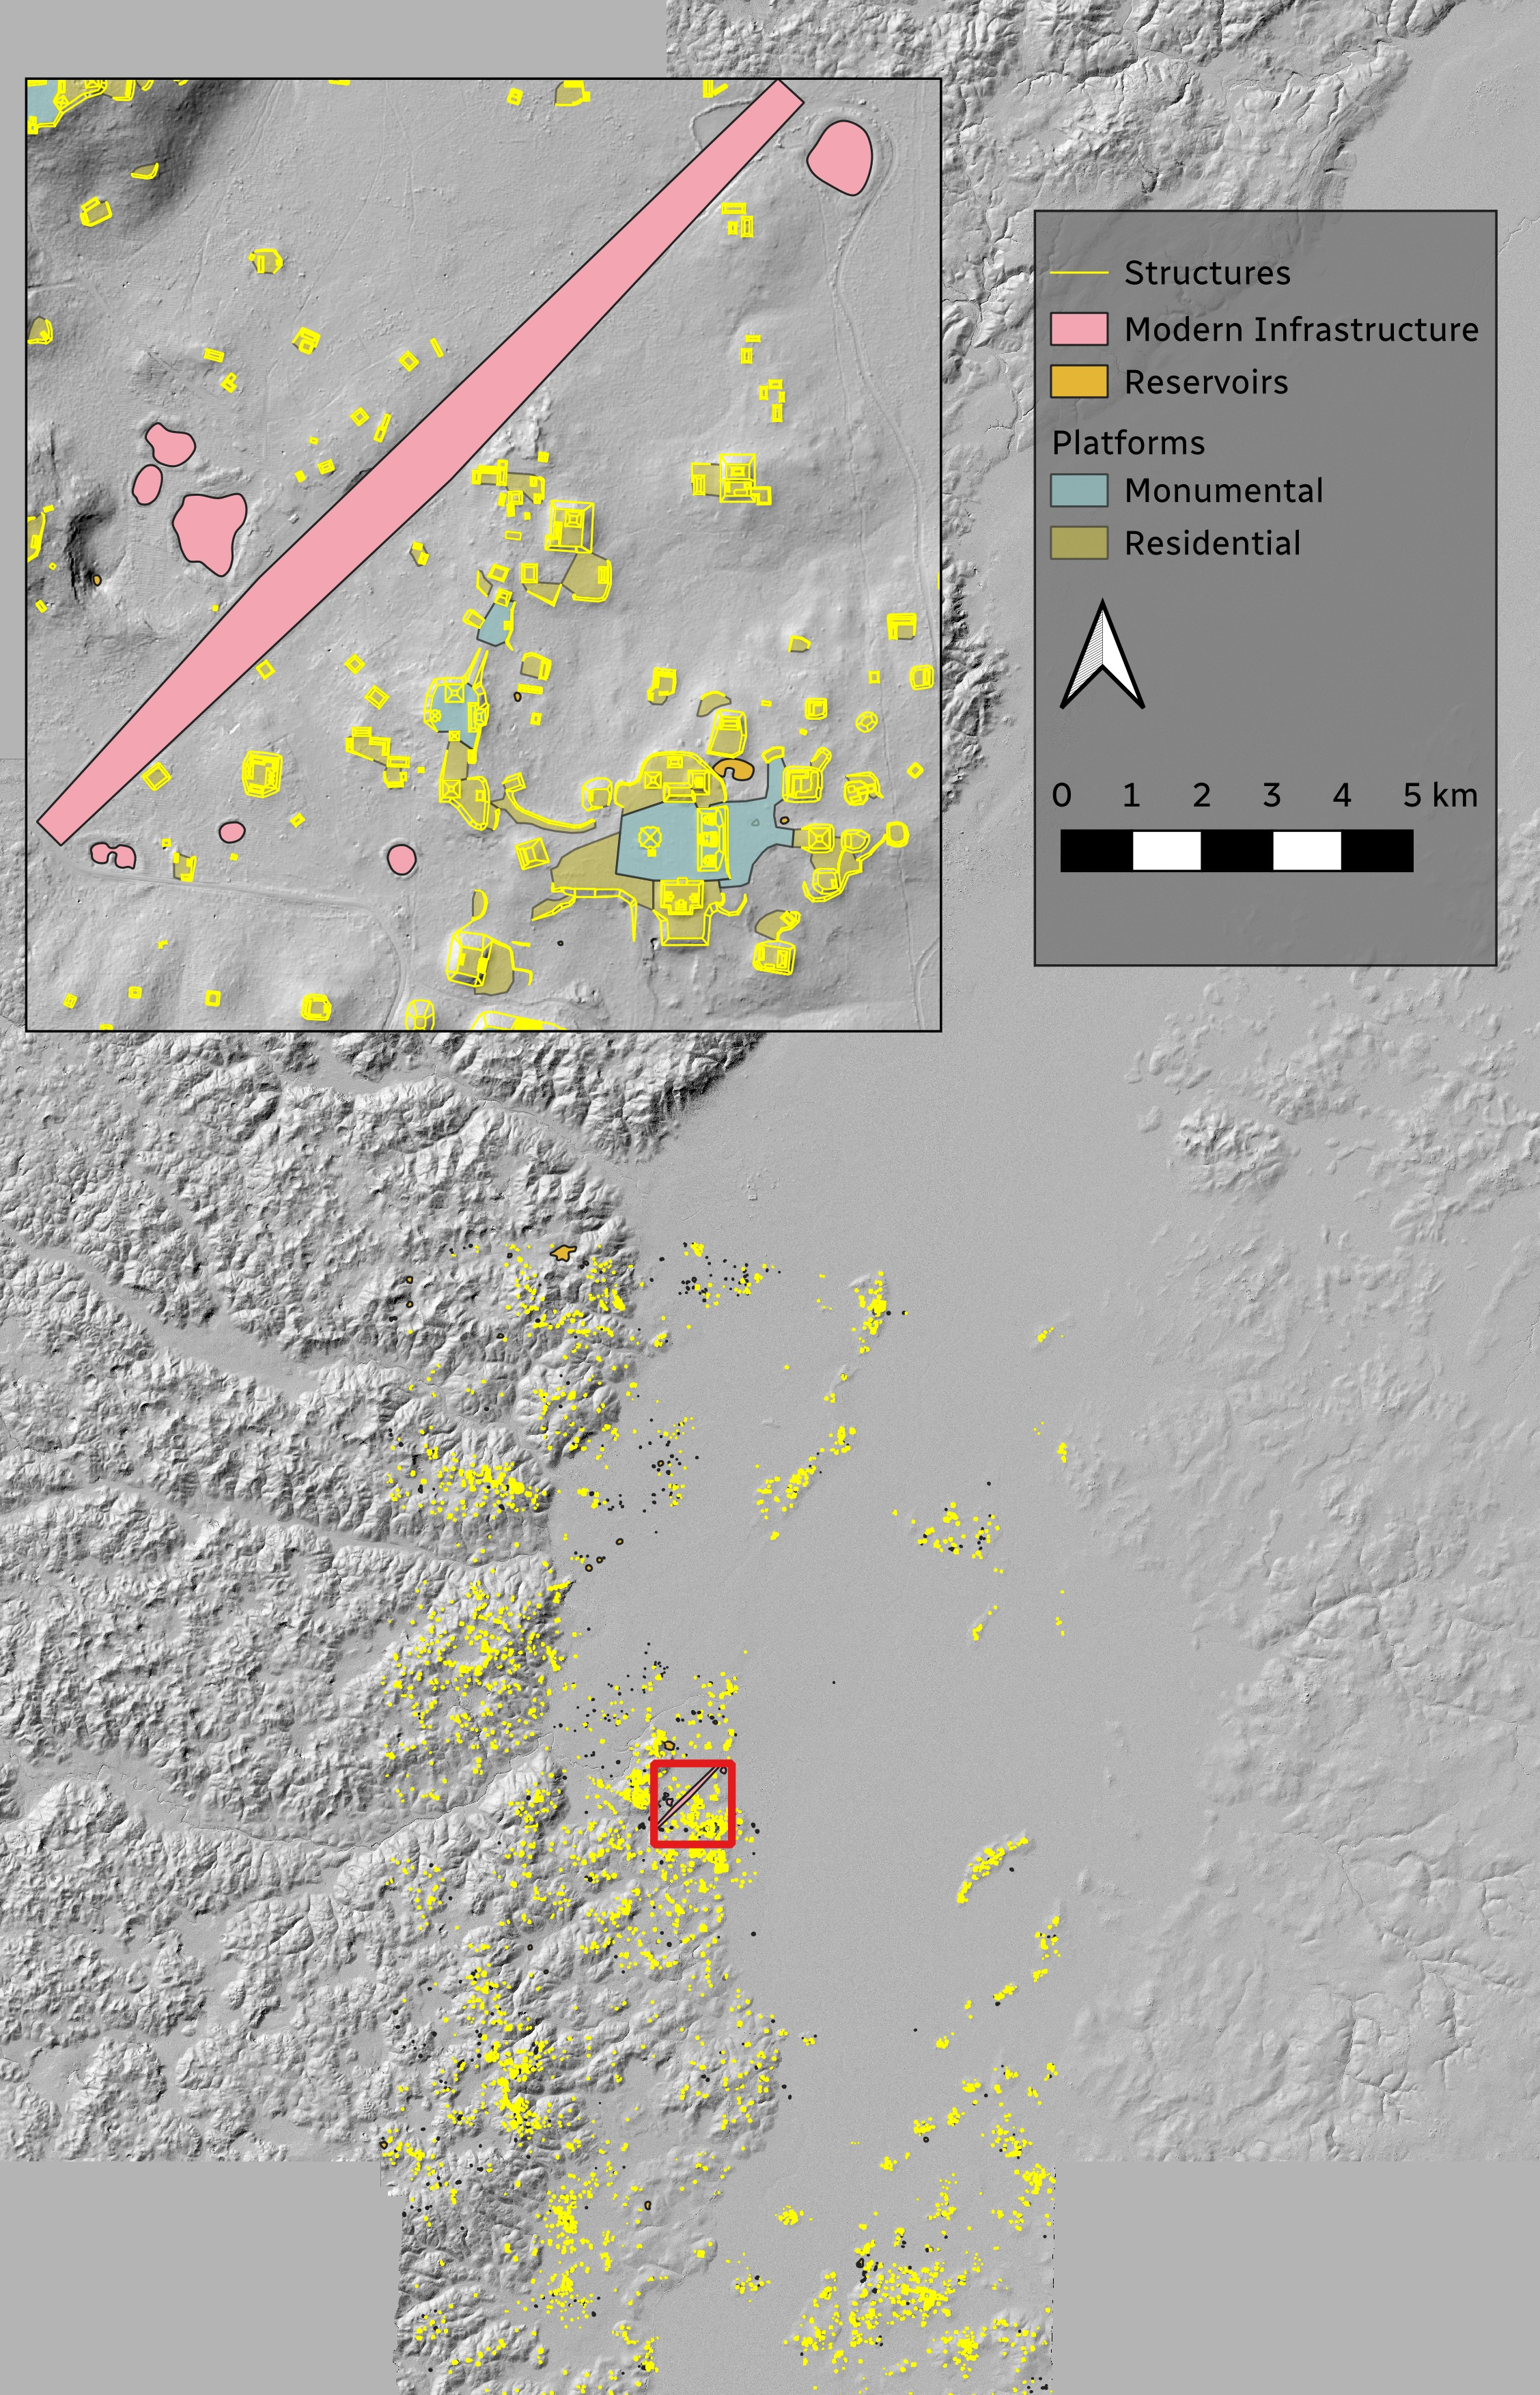
\includegraphics[width=\textwidth]{figures/DEM21_Full_Map.jpg}
	\caption{Overview of the available Maya LiDAR data used in the research.}
	\label{fig:maya_map_overview}
\end{figure}

The spatial extent of the Maya LiDAR data used in this thesis is shown in Figure~\ref{fig:maya_map_overview}. For descriptive analysis, the annotated archaeological structures were divided into three size categories:
\begin{itemize}
    \item \textbf{Small structures} --- structures covering less than 50~m\textsuperscript{2}.
    \item \textbf{Medium-sized structures} --- structures covering between 50 and 200~m\textsuperscript{2}.
    \item \textbf{Large structures} --- complex structures covering more than 200~m\textsuperscript{2}, often formed by platforms and associated construction remains.
\end{itemize}

\begin{figure}[htbp]
	\centering
	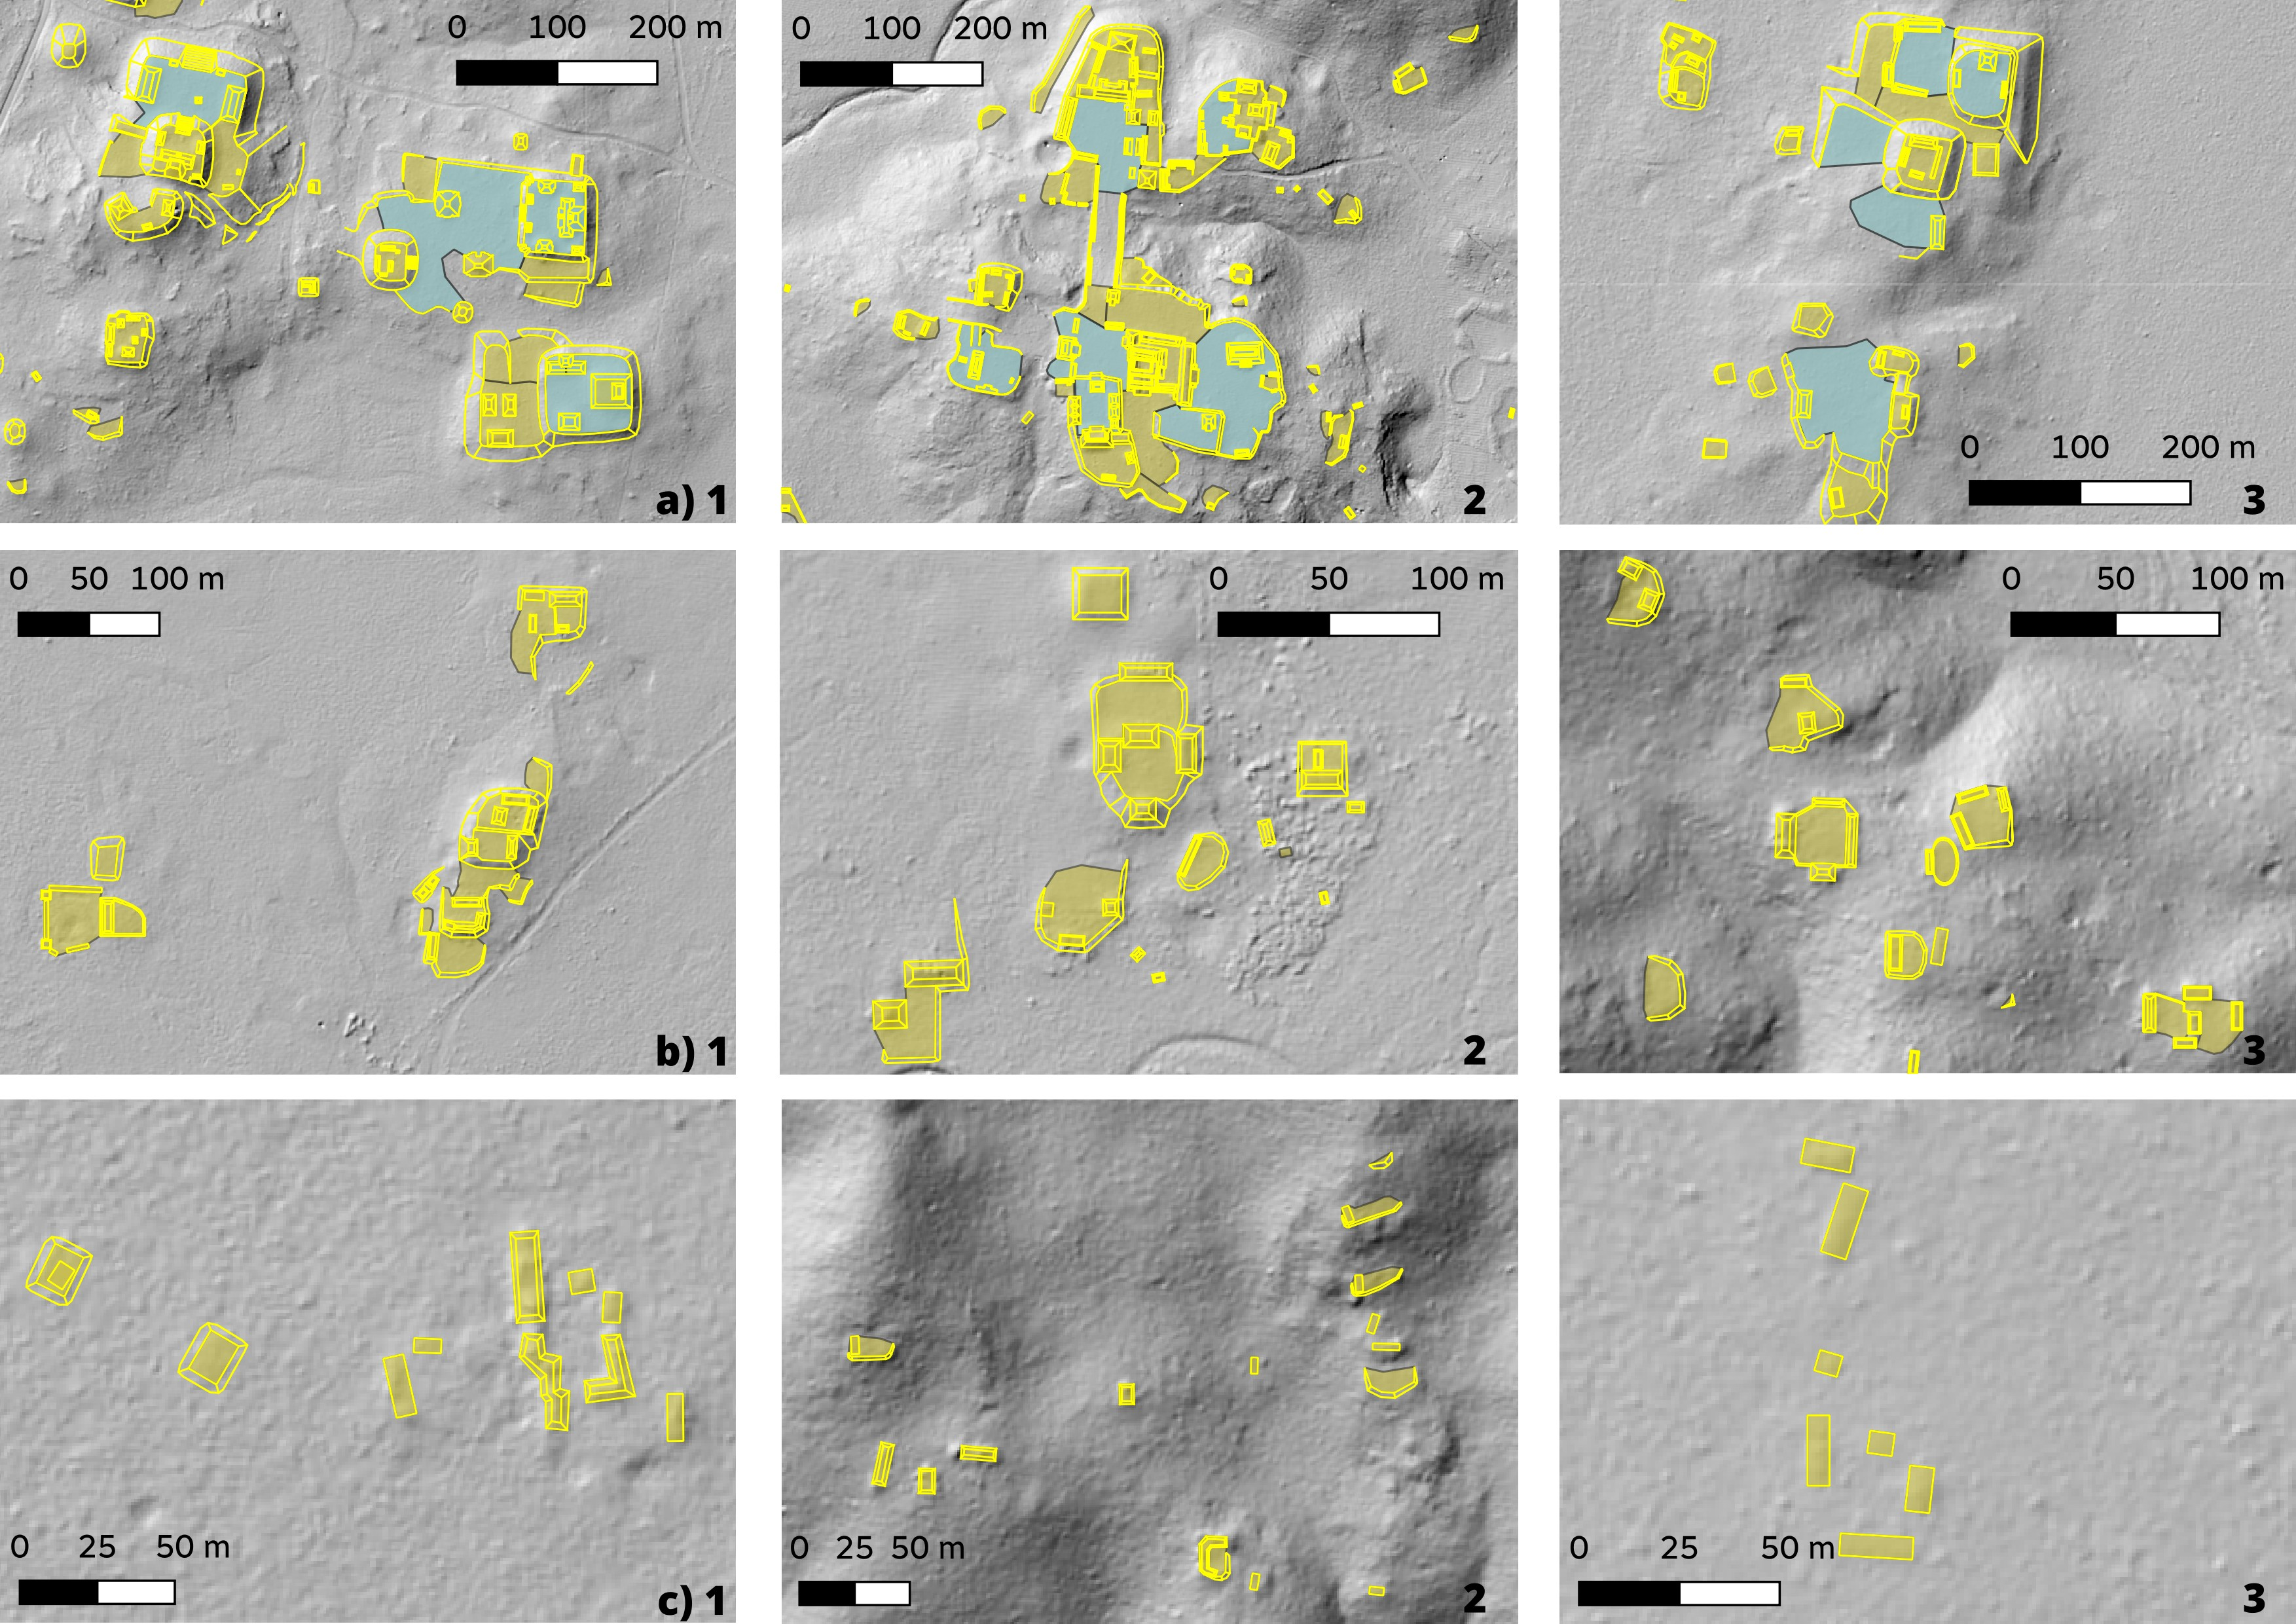
\includegraphics[width=\textwidth]{figures/Maya_Big_Medium_Small_Buildings.jpg}
	\caption{Examples of Maya structures by size category: a) large structures (\textgreater{}200~m\textsuperscript{2}), b) medium-sized structures (50--200~m\textsuperscript{2}), and c) small structures (\textless{}50~m\textsuperscript{2}).}
	\label{fig:maya_structures_visualization}
\end{figure}

\begin{table}[htbp]
\centering
\begin{tabular}{lrrrr}
\hline
Size category & Count & Total area (m\textsuperscript{2}) & Objects (\%) & Map area (\%) \\ \hline
Small  & 1491 & 47756  & 36.15 & 0.028537 \\
Medium & 2164 & 211519 & 52.47 & 0.126395 \\
Large  & 469  & 192608 & 11.37 & 0.115094 \\ \hline
\end{tabular}
\caption{Distribution of Maya archaeological structures by size category and their coverage within the mapped area.}
\label{tab:maya_structures_size}
\end{table}

\begin{figure}[htbp]
	\centering
	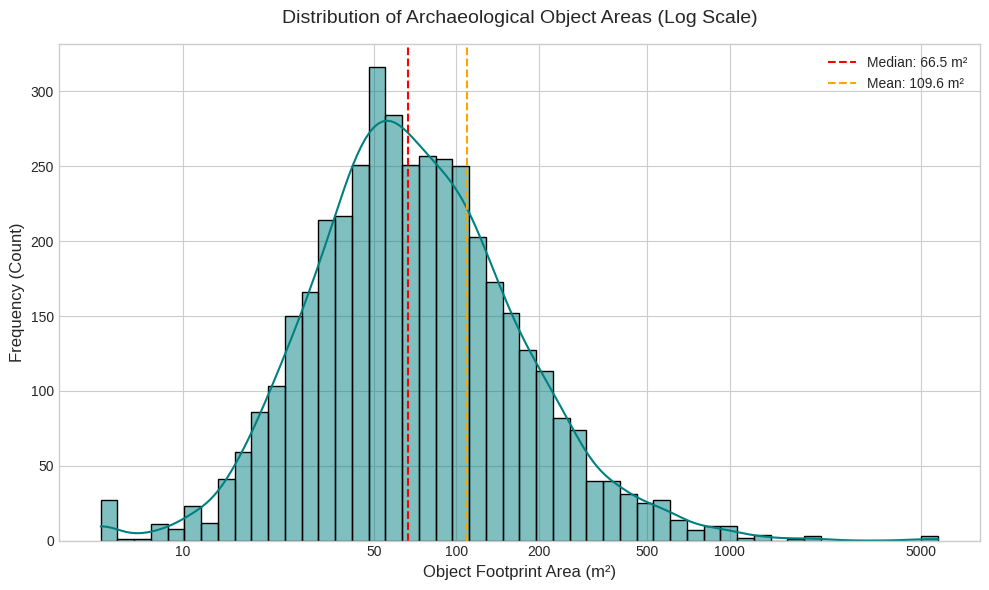
\includegraphics[width=\textwidth]{figures/maya_objects_distribution.png}
	\caption{Distribution of Maya archaeological structures by size category within the mapped area.}
	\label{fig:maya_structures_histogram}
\end{figure}

Figure~\ref{fig:maya_structures_visualization} illustrates the visual appearance of structures from the three size categories. In total, 4,124 structures were identified in the mapped area. Their distribution is summarized in Table~\ref{tab:maya_structures_size} and visualized in Figure~\ref{fig:maya_structures_histogram}. Medium-sized structures form the largest group, representing slightly more than half of all annotated objects.

\subsection{Slovak LiDAR Data}

The Slovak LiDAR data used in this thesis were provided by the Slovak University of Technology in Bratislava, Faculty of Civil Engineering (STU, StF), in cooperation with the Department of Archaeology of the Monuments Board of the Slovak Republic. This dataset represents a second, independent geographical and archaeological context, complementing the Maya data from Guatemala. While the Guatemalan data focus mainly on ancient Maya buildings and construction activity, the Slovak data are oriented toward the detection of archaeological terrace systems in Central European terrain.

The Slovak dataset contains four locations: Ladzany, Sitno, \v{S}\'{a}\v{s}ovsk\'{e} Podhradie, and Tribe\v{c}. All locations except Tribe\v{c} include reference annotations in the form of vector polylines representing the central lines of terraces. The raster resolution is 0.25~m per pixel, which is four times finer in linear resolution than the 1~m Maya DEM. This higher resolution is important for terrace detection, because terraces are narrow and elongated micro-relief structures whose visibility may be strongly affected by the spatial resolution of the raster data.

\begin{figure}[p]
    \centering

    \begin{minipage}[c][0.76\textheight][c]{0.39\textwidth}
        \centering
        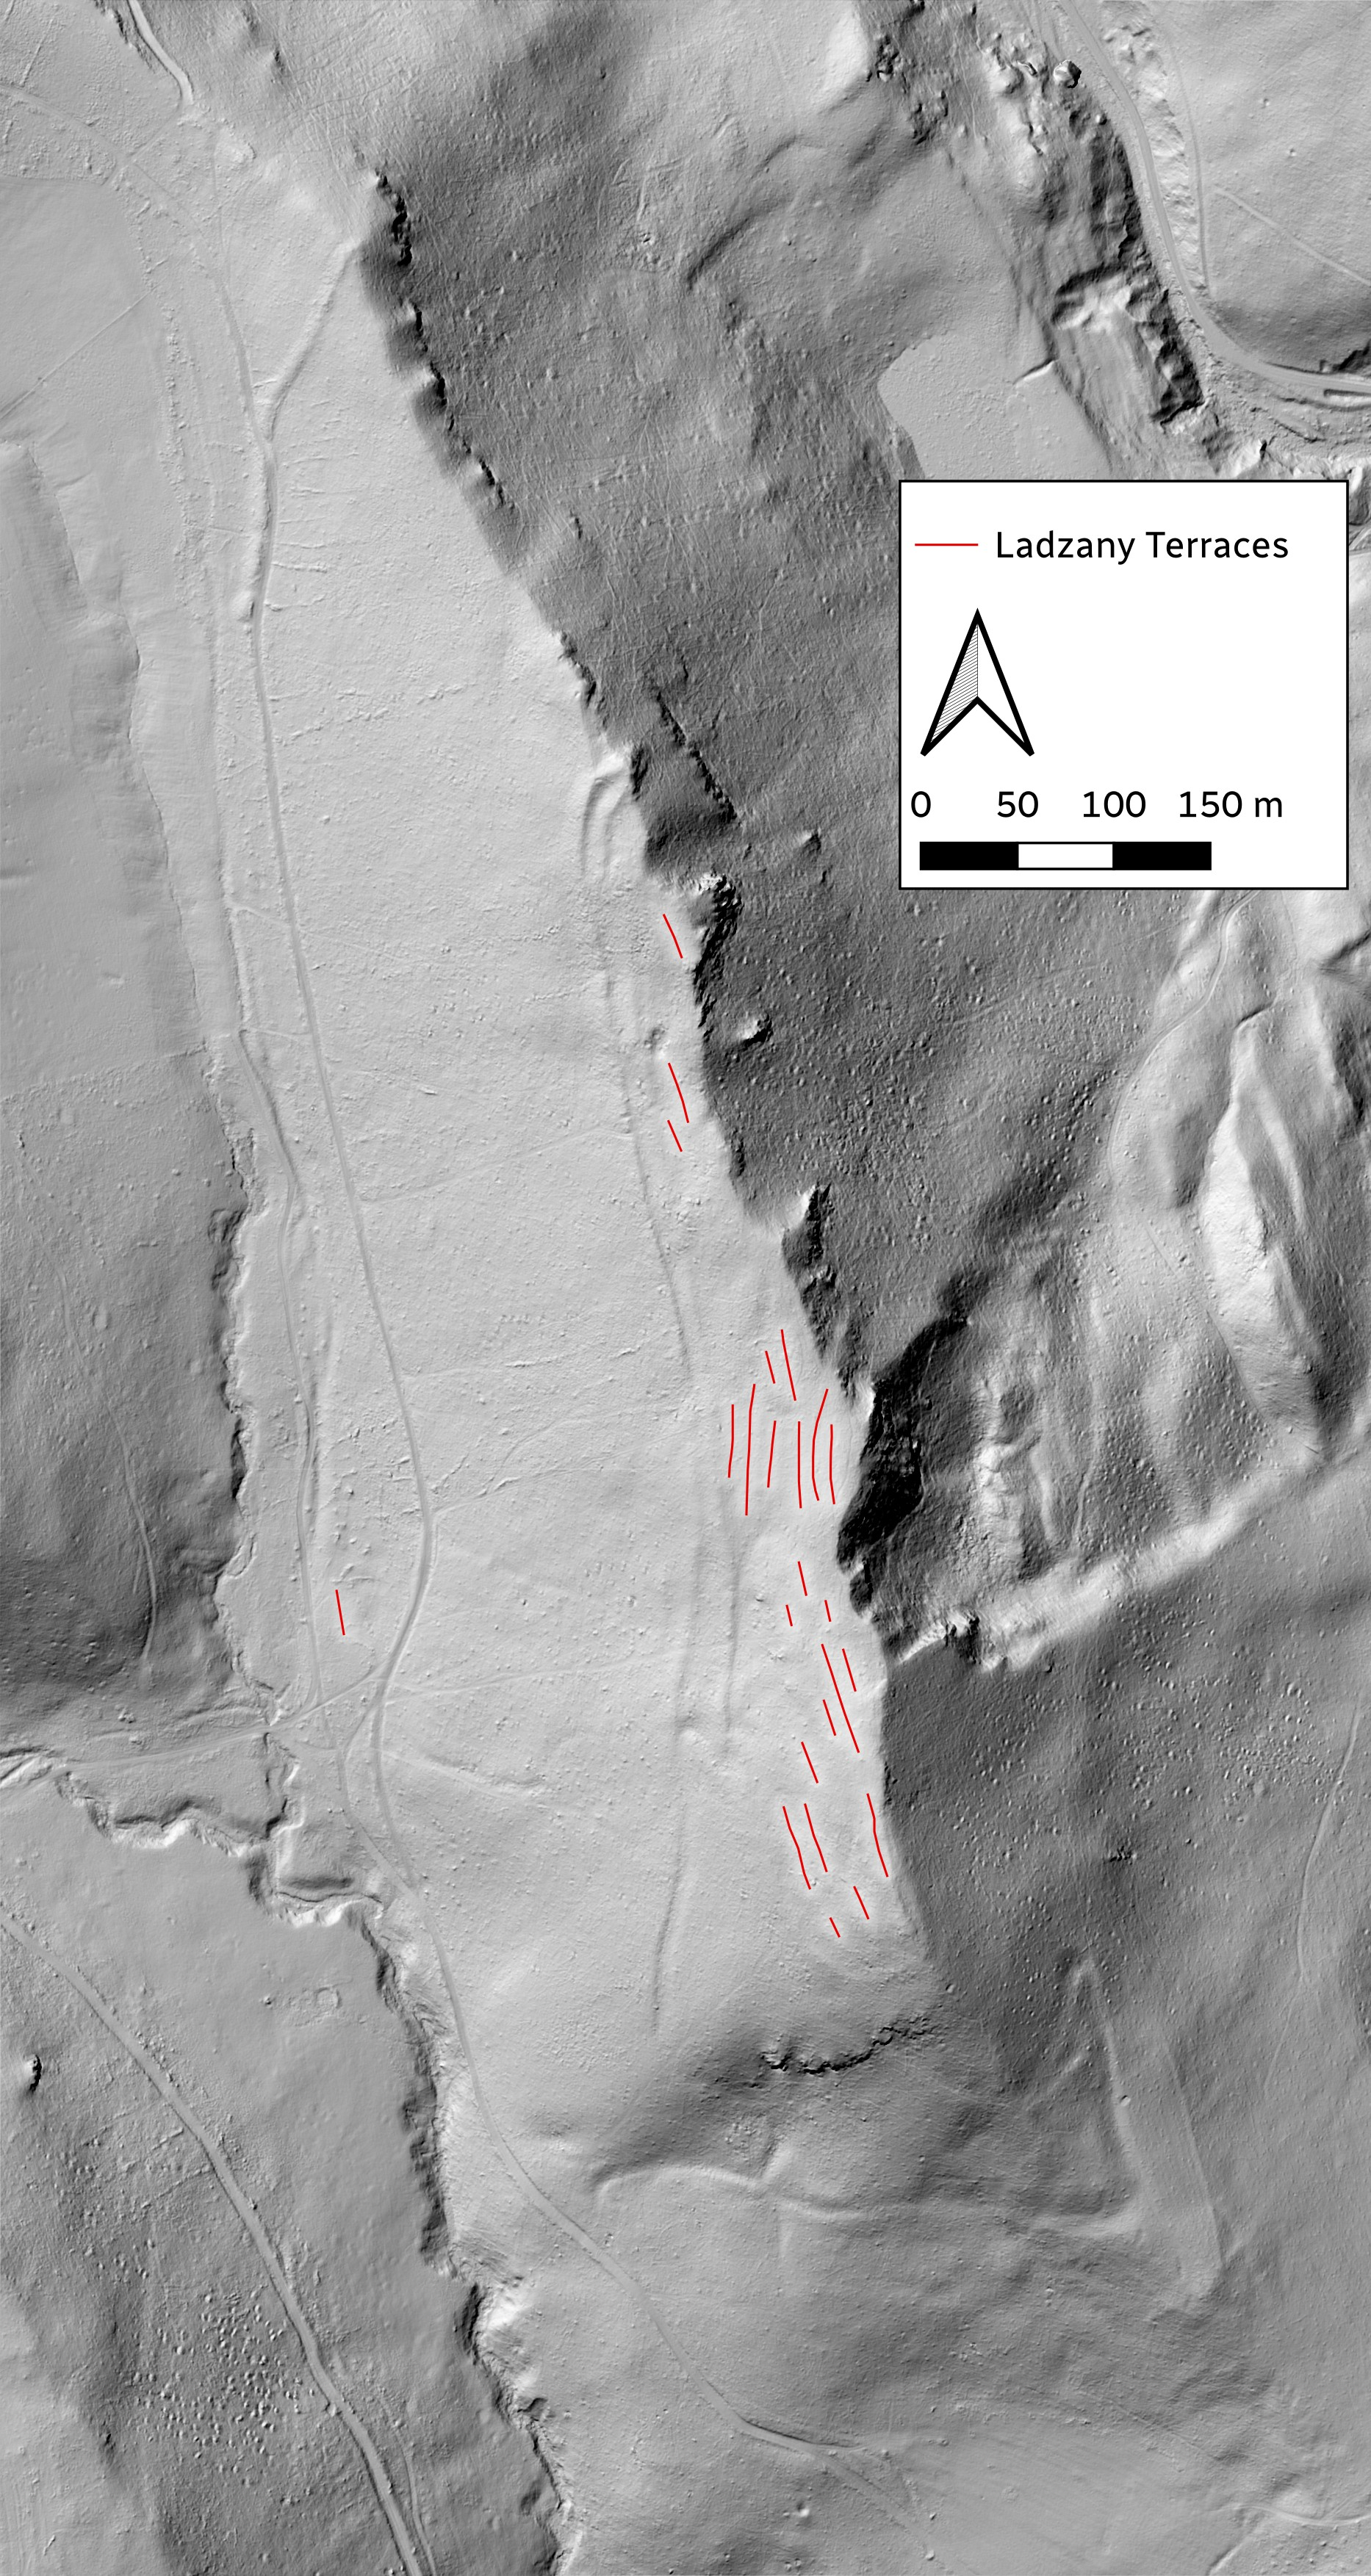
\includegraphics[
            width=\linewidth,
            height=0.62\textheight,
            keepaspectratio
        ]{figures/Ladzany_Full_Map.jpg}
    \end{minipage}
    \hspace{4mm}
    \begin{minipage}[c][0.76\textheight][c]{0.52\textwidth}
        \centering
        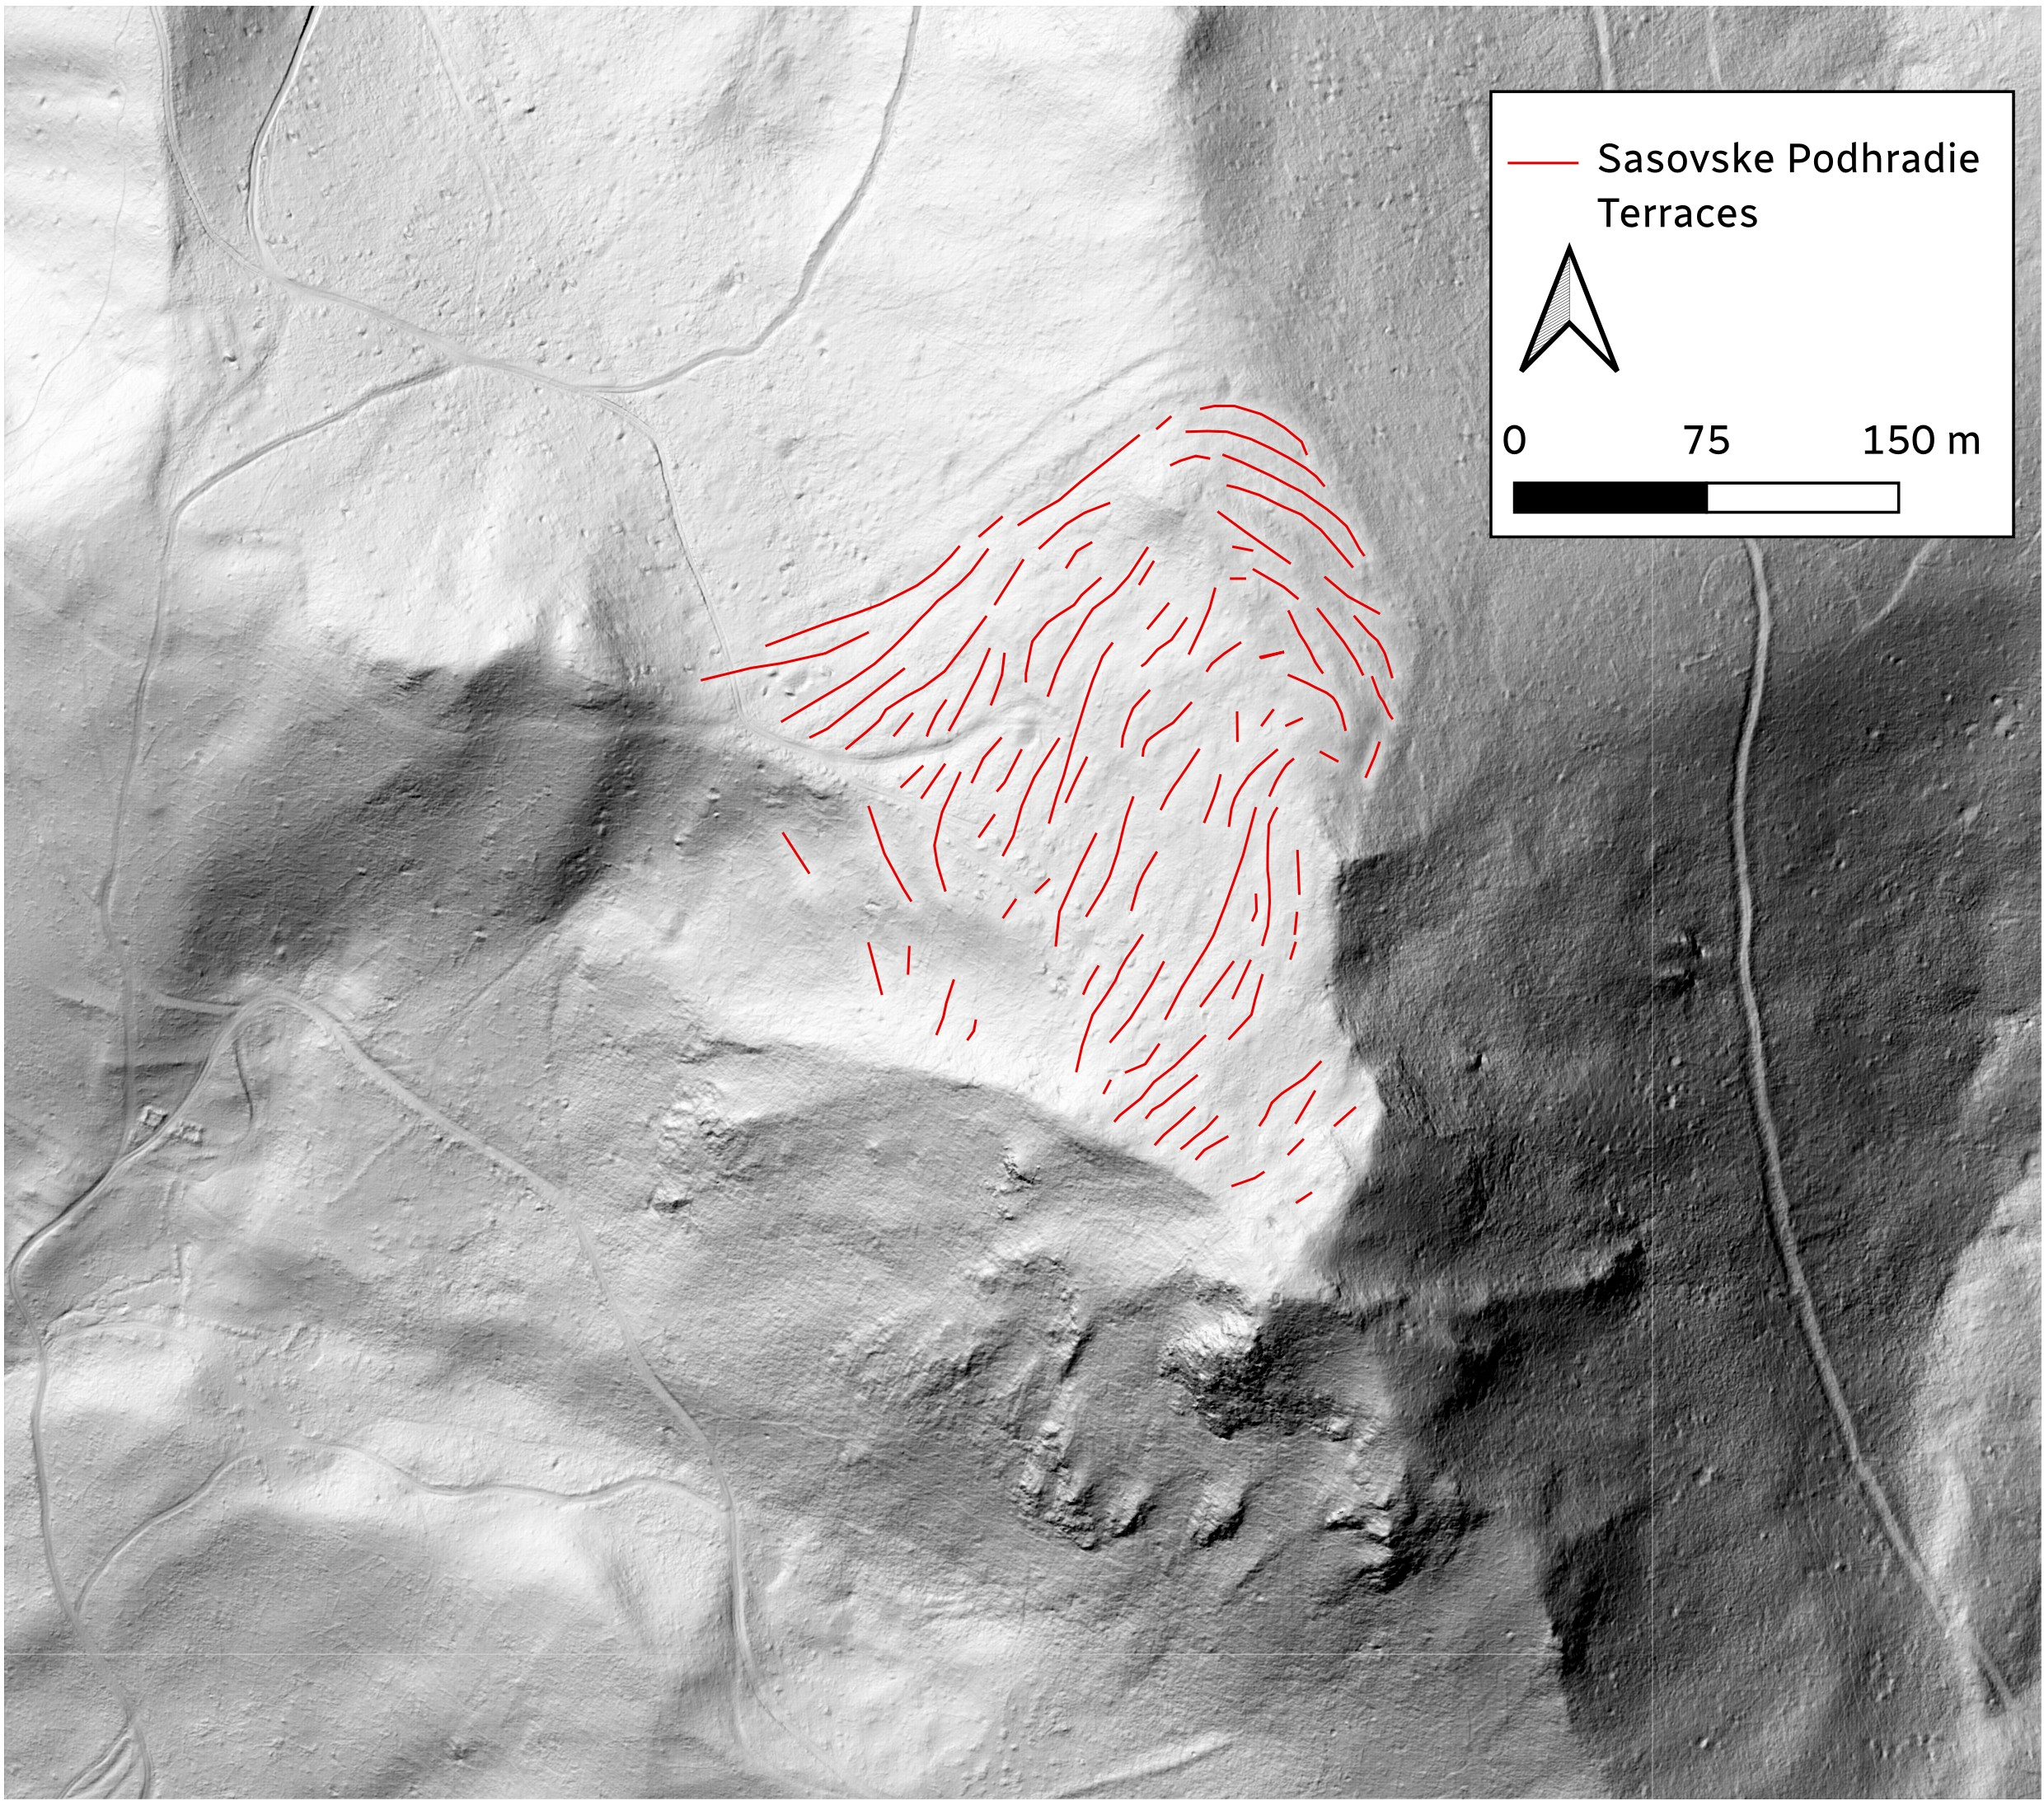
\includegraphics[
            width=\linewidth,
            height=0.22\textheight,
            keepaspectratio
        ]{figures/Sasovske_Full_Map.jpg}

        \vspace{2mm}

        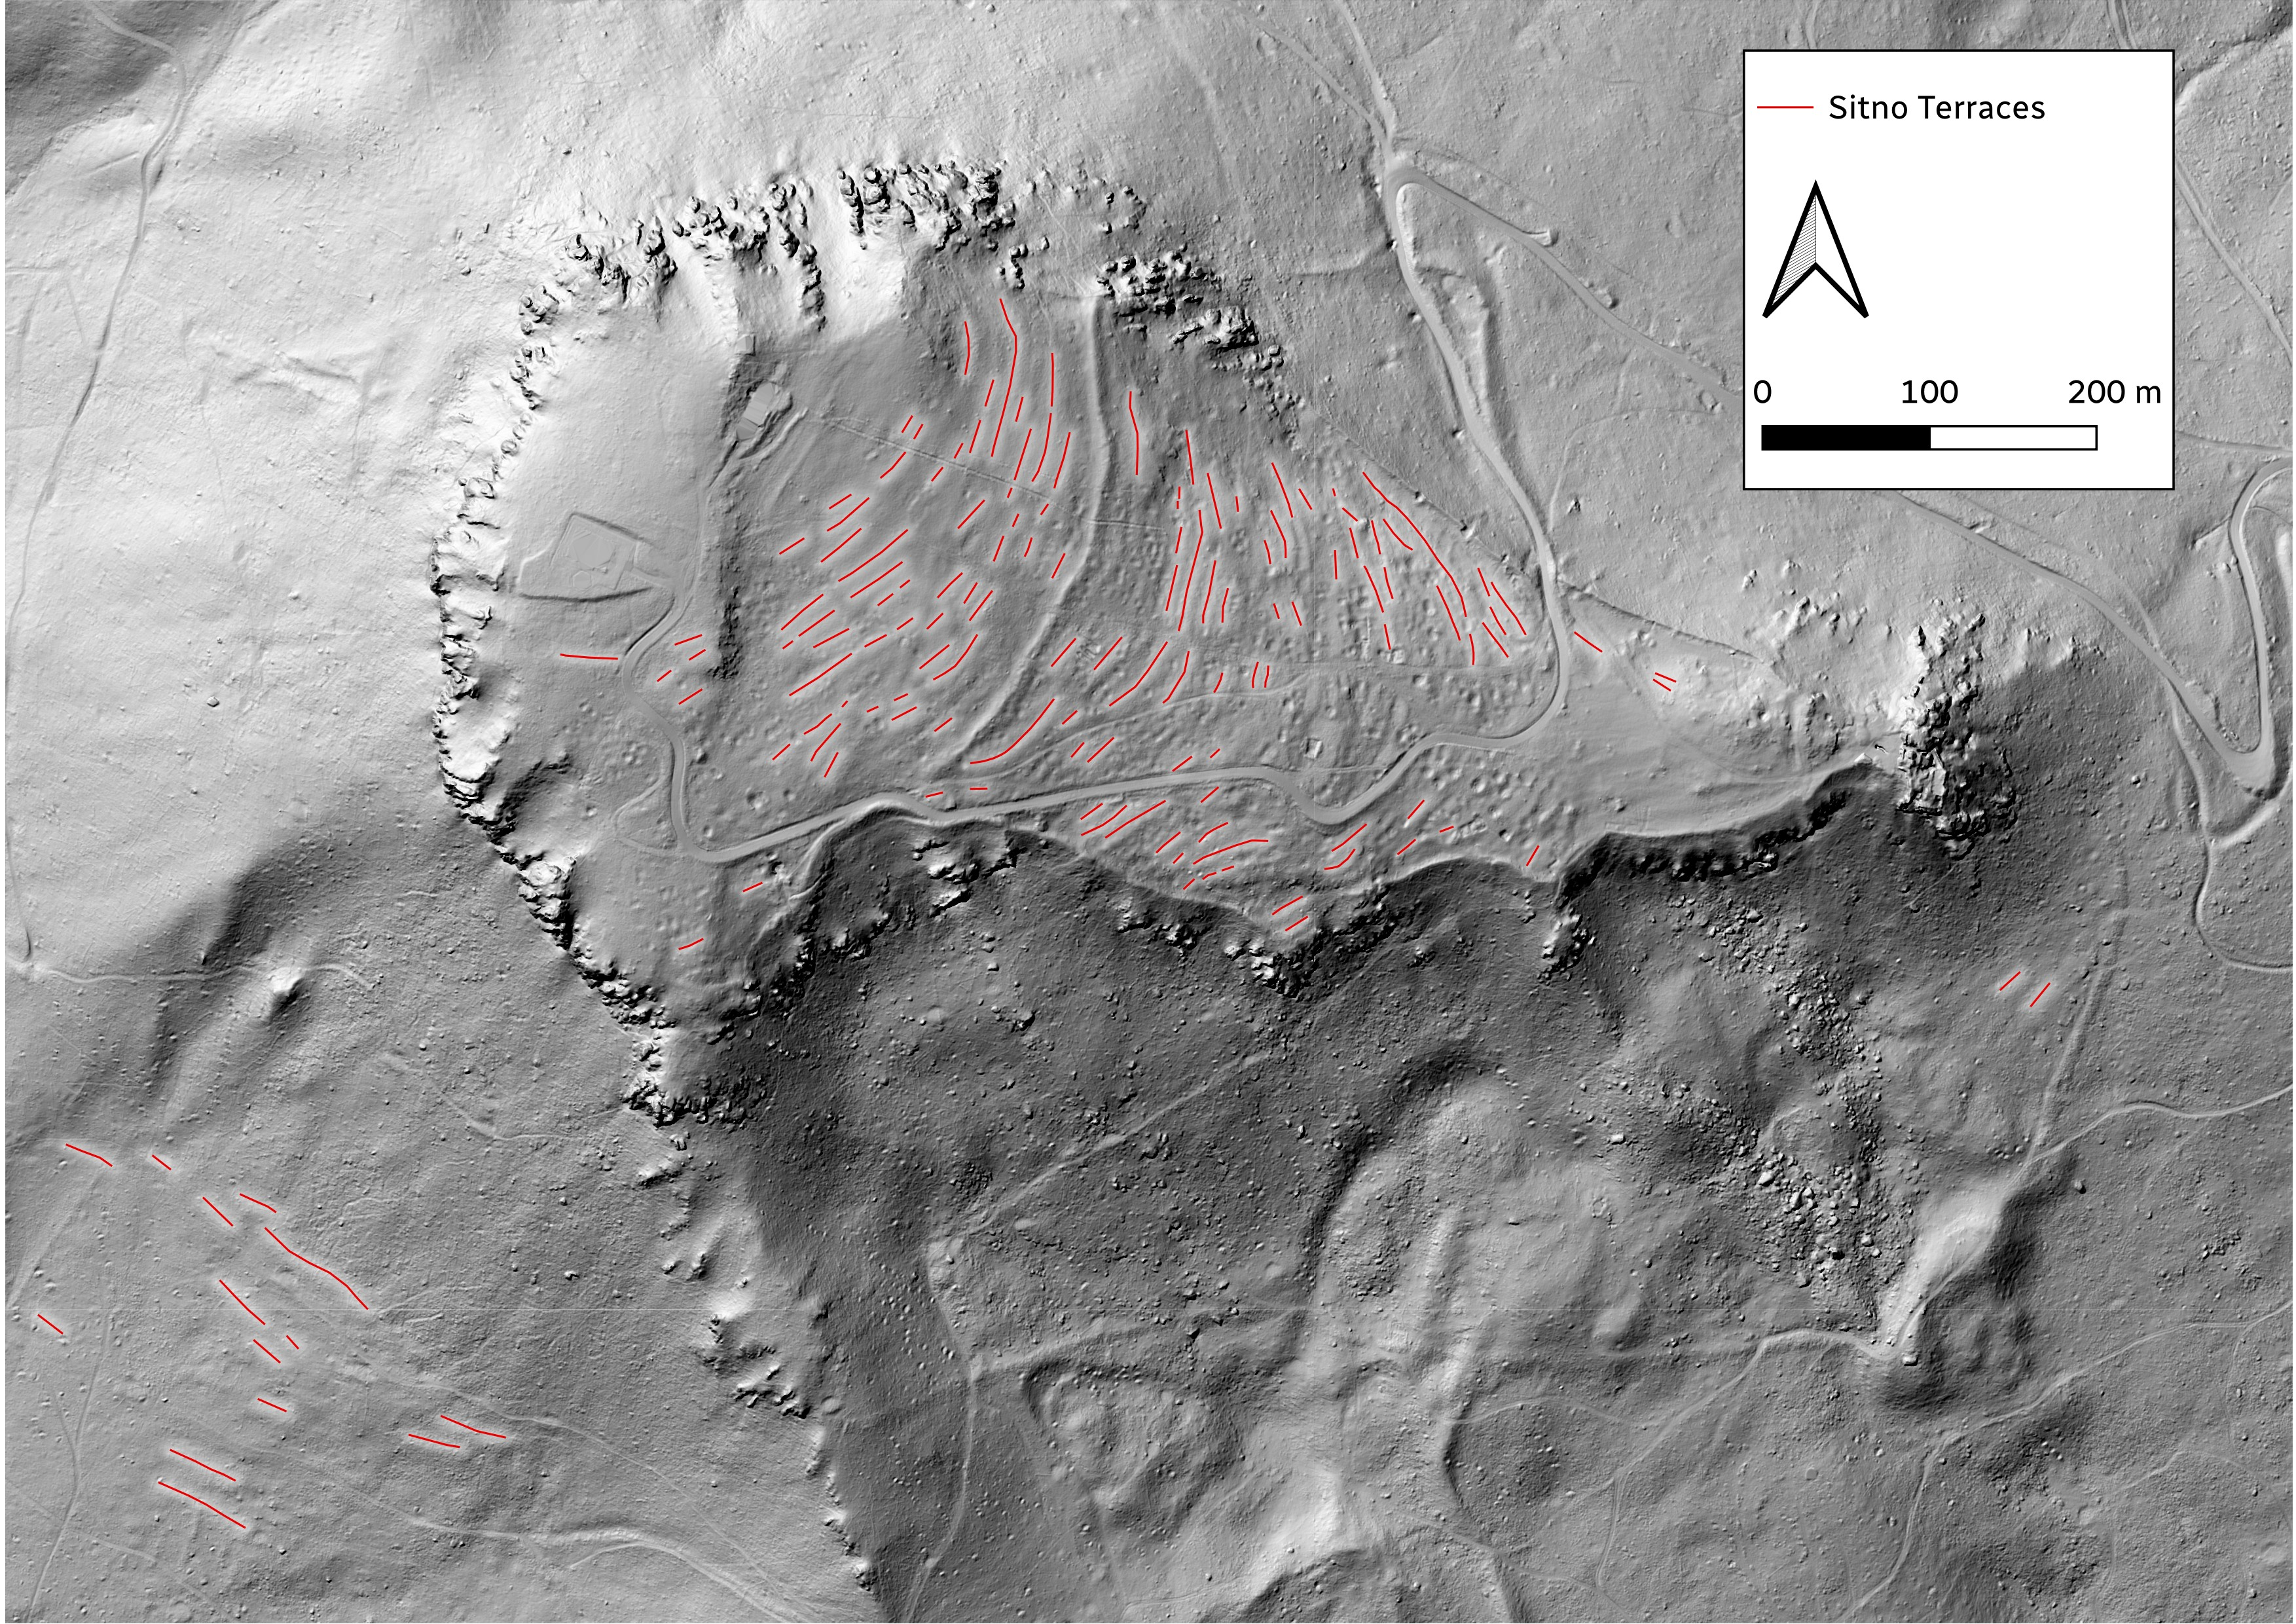
\includegraphics[
            width=\linewidth,
            height=0.22\textheight,
            keepaspectratio
        ]{figures/Sitno_Full_Map.jpg}

        \vspace{2mm}

        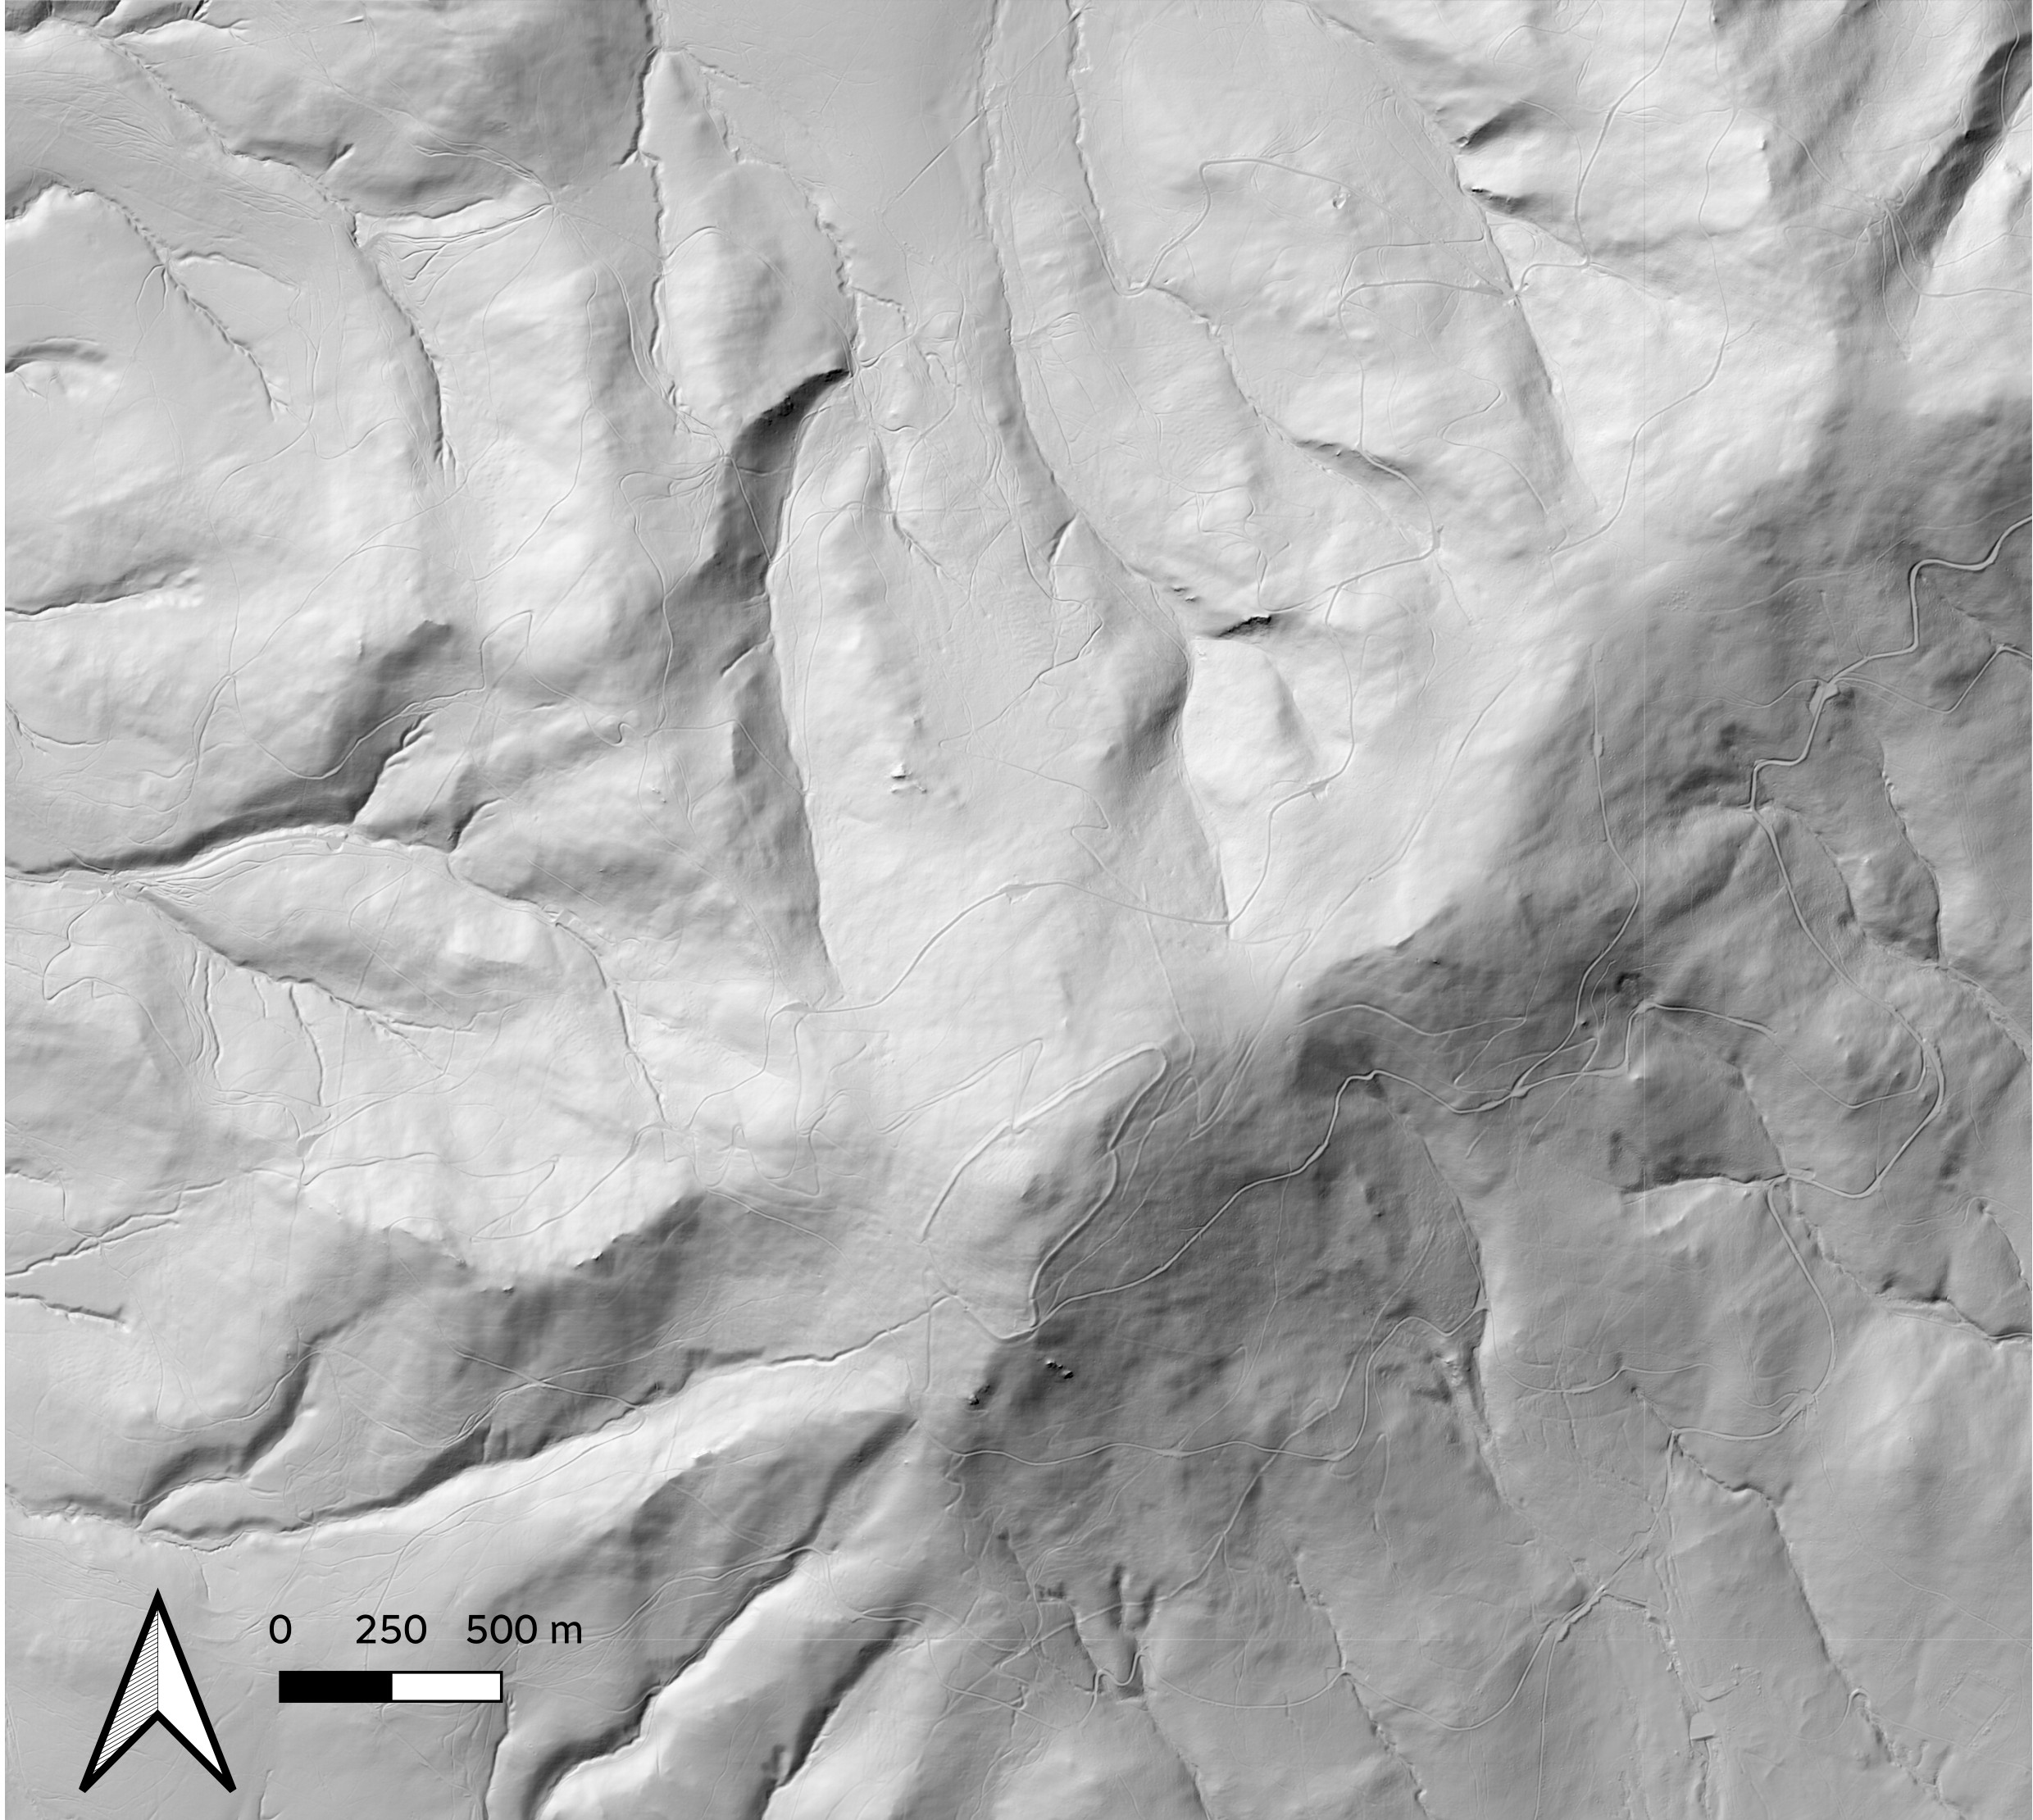
\includegraphics[
            width=\linewidth,
            height=0.22\textheight,
            keepaspectratio
        ]{figures/Tribec_Full_Map.jpg}
    \end{minipage}

    \caption{Overview of the available Slovak LiDAR datasets used in the research.}
    \label{fig:slovak_lidar_data_views}
\end{figure}

\section{Reference Data and Label Preparation}

The preparation of reference annotations has a direct influence on the quality of semantic segmentation and on the stability of model training. Archaeological annotations are not always equivalent to exact machine-learning ground truth. They are produced through expert interpretation and can therefore contain uncertainty, conservative boundaries, simplified geometry, or systematic bias. In the case of LiDAR archaeology, this problem is especially important because the model is trained on the relationship between a rasterized terrain representation and the corresponding annotation mask.

A known issue in the Maya dataset is the so-called \textit{malerization}, where LiDAR-visible archaeological structures are redrawn into schematic forms that represent their interpreted shape, size, and height. This process is useful for archaeological documentation, but it may introduce a mismatch between the idealized representation of a former structure and the actual dispersed micro-relief visible in the present terrain model~\cite{bundzel_semantic_2020}. As a result, the segmentation model may learn not only archaeological morphology, but also the conventions and imperfections of the annotation process.

\subsection{Maya Reference Masks}

For the Maya dataset, the original vector annotations were converted into raster masks aligned with the DEM grid. Two types of binary masks are available in the original methodology: the \textit{Structures} mask, containing buildings and platforms, and the \textit{Mounds} mask, containing building remains only~\cite{bundzel_semantic_2020}. In this thesis, the original binary masks are preserved as the baseline form of reference data.

Although the Maya annotations are based on expert interpretation and field verification, they are not treated as perfectly certain labels. Bundzel et al.~\cite{bundzel_semantic_2020} proposed the use of \textit{confidence shadows} to reduce the negative effect of hard and potentially uncertain object boundaries. A confidence shadow replaces a strictly binary transition at the object boundary with a gradual decrease of label confidence from 1 to 0 within a defined neighbourhood around the object. In this thesis, this idea is used to prepare additional soft-mask variants of the reference labels.

The resulting Maya reference data therefore include both binary masks and soft masks. The binary masks are used to preserve the original expert annotation, while the soft masks are used to test whether smoother boundary supervision improves training stability and segmentation quality.

\subsection{Slovak Terrace Masks}

The Slovak reference annotations differ from the Maya annotations in both geometry and interpretation. Instead of polygonal object boundaries, the terrace annotations are available as vector polylines representing the approximate central lines of terraces. Direct rasterization of these polylines would produce extremely thin masks. At a resolution of 0.25~m per pixel, such one-pixel-wide labels would be too sparse for stable training and would not represent the possible physical width of the terrace feature.

For this reason, the Slovak terrace annotations were buffered before rasterization. Each terrace polyline was expanded by 2~m, corresponding to 8 pixels at 0.25~m resolution, on each side of the central line. This buffering was used as a compromise between preserving the original annotation geometry and creating a learnable target area for semantic segmentation. The polyline endpoints were rounded during buffering in order to avoid artificial rectangular endings in the rasterized mask.

As in the Maya dataset, two label variants were prepared for the Slovak terrace data. The first variant is a binary mask obtained from the buffered terrace annotations. The second variant is a soft mask based on the same buffered geometry, where the label confidence decreases gradually near the boundary. These two variants make it possible to compare the effect of hard and soft supervision on the segmentation of elongated archaeological features.

\section{LiDAR-Derived Input Representations}\label{sec:lidar_input_representations}

A Digital Elevation Model (DEM) stores absolute elevation values and therefore provides the primary terrain representation derived from LiDAR data. However, archaeological features are often expressed as subtle local micro-relief variations rather than as large absolute elevation differences. For this reason, direct use of the DEM can be insufficient, especially in areas where local archaeological structures are visually suppressed by broader terrain variation, slope, or regional elevation trends. Derived LiDAR visualizations are therefore used to enhance local topographic patterns and to make anthropogenic micro-relief more distinguishable.

The input representations used in this thesis can be divided into two main groups. The first group consists of numerical terrain-derived representations, such as the DEM itself and derivative layers computed from elevation values. These representations preserve a direct relationship to the terrain surface and can be interpreted as continuous geospatial data. The second group consists of image-like raster visualizations designed primarily to emphasize visual contrast, relief edges, and local topographic forms. Such visualizations are commonly used in archaeological interpretation because they make small terrain anomalies easier to inspect visually.

Several basic LiDAR-derived visualizations and terrain derivatives were discussed in Chapter~\ref{ch:analysis}. Individually, each representation emphasizes only a specific aspect of the terrain. For example, hillshade provides an intuitive visual impression of relief, but it depends on the selected illumination direction and can therefore introduce orientation bias. Slope highlights changes in elevation, while sky-view factor and positive openness provide alternative descriptions of local terrain visibility and openness that are less dependent on a single illumination angle~\cite{thompson_detecting_2020,kokalj_standardizing_2025}.

For deep learning, a single representation may not provide sufficient contextual information. Therefore, multi-channel combinations are often used to combine complementary terrain properties in one input tensor. A relevant example is the SPS representation, which combines Slope, Positive Openness, and Sky-View Factor into a three-channel image. This representation has been used in recent work on Maya LiDAR segmentation because it combines local gradient information with illumination-independent topographic descriptors and is suitable for CNN-based processing~\cite{zhang_unveiling_2024}.

In this thesis, all input representations are converted into a three-channel format. This decision has two practical advantages. First, it allows different LiDAR-derived layers to be combined in a controlled way. Second, it makes the input compatible with standard convolutional architectures and pre-trained backbones that are commonly designed for three-channel image inputs. This is especially useful when using models whose encoders were originally trained on natural image datasets.

The representations used in this thesis can be grouped into three categories:
\begin{enumerate}
    \item \textbf{Numerical elevation-derived representations} computed directly from the original DEM data. These representations preserve a numerical relationship to the terrain surface and are therefore treated as continuous geospatial inputs.
    
    \item \textbf{Image-like RGB visualizations} derived from LiDAR data. These representations do not preserve the original numerical elevation relationships directly. Instead, they encode terrain information as a combination of three colour channels and are primarily useful for emphasizing relief contrast, object boundaries, and visually interpretable micro-relief patterns.
    
    \item \textbf{Hybrid representations} combining image-like raster visualization channels with numerical elevation-derived data. In this case, one of the RGB channels is replaced by a numerical terrain representation in order to test whether the model benefits from combining visual contrast with direct terrain information.
\end{enumerate}

Based on this categorization, the following input representations were used in the experiments:
\begin{enumerate}
    \item \textbf{DEM} --- the original Digital Elevation Model used as the most direct terrain-based baseline. Since the DEM is a single-channel raster, it was converted into a three-channel input by repeating the same normalized elevation layer across all three channels.

    \item \textbf{RGB} --- a three-channel raster visualization derived from LiDAR data. This representation is used as an image-like input intended to approximate the type of visually enhanced terrain representation used during manual inspection. 

    \item \textbf{RGDEM} --- a hybrid representation combining the red and green channels from the RGB visualization with the DEM as the third channel. This representation was introduced to preserve part of the visual contrast from the RGB raster while adding explicit elevation information from the DEM. Since this representation combines image-like and numerical channels, z-score normalization was applied as described in Section~\ref{sec:dataset_construction}.

    \item \textbf{SPS} --- a three-channel numerical representation composed of Slope, Positive Openness, and Sky-View Factor. Each channel was computed separately from the original DEM. This representation was included because it combines local gradient information with illumination-independent topographic descriptors and has been shown to be suitable for CNN-based processing of archaeological LiDAR data~\cite{zhang_unveiling_2024}.

    \item \textbf{ISO} and \textbf{ANISO} --- raster representations used only for the Slovak terrace dataset. They were included because the Slovak terrace task involves narrow elongated structures, for which different isotropic and anisotropic visual enhancement strategies may affect feature visibility.

\end{enumerate}

The DEM, RGB, RGDEM, and SPS representations were used as the main input variants for the Maya dataset. For the Slovak terrace dataset, the same general experimental logic was preserved, but the ISO and ANISO representations were mainly used because they were available for this dataset and were expected to be relevant for elongated terrace-like features.

\section{Dataset Construction}\label{sec:dataset_construction}

To ensure reproducibility and consistency, all derived datasets were created using the same storage structure and processing logic. The dataset format was kept independent of the specific input representation. Therefore, experiments using different terrain derivatives or raster visualizations could be performed without changing the training pipeline itself.

Each dataset sample consists of four main components:
\begin{enumerate}
    \item the input raster data in three-channel format;
    \item a binary segmentation mask;
    \item an optional soft mask;
    \item a valid pixel mask.
\end{enumerate}

The input raster contains the three-channel representation used by the segmentation model. The binary mask defines the target class as archaeological structure or background. The soft mask, when used, provides a continuous version of the target mask with gradually decreasing confidence near object boundaries. The valid pixel mask indicates which pixels belong to valid data areas and must be used during training and evaluation.

For DEM-based inputs and numerical terrain-derived representations, z-score normalization was applied independently to each input channel. The mean and standard deviation were computed only from valid pixels, using the valid pixel mask. This prevents missing-data regions from affecting the normalization statistics and reduces the risk of scale distortion caused by invalid values. After normalization, invalid pixels were assigned the value 0. In the normalized representation, this value corresponds to the mean of the valid data and therefore provides a neutral fill value for areas excluded from training and evaluation.

Image-like raster visualizations already have a bounded display-oriented value range. Therefore, they do not necessarily require the same normalization as raw elevation-derived data. However, when image-like visualizations are combined with numerical terrain derivatives, normalization is required to reduce differences in value scale between channels. In such mixed representations, z-score normalization was applied to ensure that no channel dominated the model input only because of its numerical range.

% TODO: Verify the final normalization rule used in the implementation. If RGB-like raster visualizations were kept in [0,1] or [0,255], state it explicitly. If all channels were normalized with z-score regardless of representation type, simplify this paragraph accordingly.

The segmentation masks and soft masks were stored as separate matrices. The binary mask was used for hard supervision and for final evaluation, while the soft mask was used only in experiments where soft supervision was explicitly enabled. The valid pixel mask was used to exclude invalid areas from loss computation and metric calculation.

\section{Model and Training Methodology}\label{sec:model_training_methodology}

The segmentation task in this thesis is formulated as binary semantic segmentation. Each valid pixel of the input raster is classified either as archaeological structure or as background. Within the scope of this thesis, DeepLabV3 and DeepLabV3+ were selected as the main segmentation architectures.

The choice of these architectures is motivated by their suitability for dense prediction tasks and by their ability to capture multi-scale spatial context. DeepLabV3 uses atrous convolution and Atrous Spatial Pyramid Pooling (ASPP), which allow the model to aggregate contextual information at multiple receptive-field scales without excessively reducing spatial resolution~\cite{chen_rethinking_2017}. This is important for archaeological LiDAR data because target objects may appear at different sizes and may be embedded in complex terrain backgrounds. DeepLabV3+ extends this idea with an encoder--decoder structure, improving the recovery of spatial detail in the final segmentation output~\cite{chen_encoder-decoder_2018}. This makes it more suitable for objects with narrow boundaries or elongated forms, such as terraces.

Compared with U-Net, DeepLab-based models provide a stronger multi-scale context module through ASPP and are widely used in remote sensing segmentation tasks. Compared with Mask R-CNN or other instance-segmentation approaches, DeepLabV3 and DeepLabV3+ are more directly aligned with the binary pixel-wise formulation used in this thesis. The goal is not to separate individual archaeological instances, but to produce a continuous segmentation mask indicating areas likely to correspond to archaeological features.

% TODO: If U-Net was not experimentally tested in this thesis, keep the comparison brief as above. If U-Net was tested as a baseline, this paragraph should be rewritten to describe it as part of the experimental setup rather than as an excluded alternative.

The original LiDAR rasters are too large to be processed by the neural network as complete images. Therefore, the data were divided into smaller tiles. A manifest-based dataset construction strategy was used to make this process reproducible. Instead of permanently creating separate physical datasets for every experiment, each manifest stores the spatial coordinates of tiles, their dataset split, and relevant metadata. During training or validation, the corresponding tile is loaded from the selected input representation using the coordinates stored in the manifest.

This approach makes the dataset split independent of the input representation. Since the segmentation masks and valid pixel masks are aligned with the source raster grid, the same manifest can be reused for different input representations of the same study area. This ensures that experiments differ only in the controlled variable being tested, such as input representation, label type, or loss function.

Due to the different spatial resolutions of the datasets, different tile sizes were used. For the Maya dataset, tiles of $128 \times 128$ pixels were used. With a spatial resolution of 1~m per pixel, each tile covers an area of $128 \times 128$~m. For the Slovak terrace dataset, tiles of $256 \times 256$ pixels were used. At a spatial resolution of 0.25~m per pixel, each tile covers an area of $64 \times 64$~m. This choice keeps the physical scale of the model input comparable between datasets while respecting their different raster resolutions.

To reduce artifacts at tile boundaries, overlapping tiles were used. The stride was set to one quarter of the tile size: 32 pixels for the Maya dataset and 64 pixels for the Slovak dataset. As a result, each interior pixel can be evaluated multiple times under different local contexts during validation and inference. The overlapping predictions are later aggregated into a single probability map, as described in Section~\ref{sec:inference_postprocessing}.

% TODO: Verify whether the implementation uses stride = tile_size / 4 or overlap = tile_size / 4. These are different. The text above assumes stride = tile_size / 4, i.e. 75% overlap.

For the Maya dataset, five spatial manifests were created following a cross-validation strategy. The annotated area was divided into five spatial folds. In each run, one fold was used for validation and the remaining four folds were used for training. A buffer of 64 pixels was introduced at the boundaries between training and validation zones to reduce spatial leakage caused by overlapping tiles. This step is important because neighbouring LiDAR tiles may contain highly similar terrain context, and without a buffer the validation metrics could be artificially inflated.

Only training tiles containing at least one positive pixel were used for training. This still preserves a large amount of background information inside each tile, but avoids training on a dataset dominated by fully empty background tiles. For validation, the entire relevant validation area was used in order to obtain metrics that reflect model behaviour on both positive and background regions.

% TODO: If negative/background-only tiles were also sampled using a fixed negative-to-positive ratio, this paragraph must be corrected. The current version assumes that only positive training tiles were used.

For the Slovak terrace dataset, a leave-one-location-out cross-validation strategy was applied. Since three labelled locations are available, each fold uses two locations for training and the remaining location for validation. This setup provides a stricter evaluation scenario than random tile-level splitting, because the validation area is geographically separated from the training areas. It also allows the experiment to assess how well the model generalizes between different Slovak terrain contexts.

The severe class imbalance between archaeological features and background is one of the main training challenges. Archaeological structures occupy only a small fraction of the raster area, and this is especially pronounced in the Slovak terrace dataset, where the target objects are narrow and elongated. For this reason, loss functions suitable for imbalanced segmentation were used and compared. The training loss was computed only over valid pixels, so that invalid or missing-data areas did not influence the optimization process.

% TODO: Insert the exact final list of loss functions used in the experiments, e.g. BCE + Dice, Focal + Dice, Tanimoto loss, or another final set. This paragraph should match Chapter~\ref{ch:design_protocol} exactly.

To increase the variability of the training data and reduce overfitting, simple geometric augmentations were applied:
\begin{enumerate}
    \item random horizontal flipping;
    \item random vertical flipping;
    \item random rotation by $0^\circ$, $90^\circ$, $180^\circ$, or $270^\circ$.
\end{enumerate}

Only geometry-preserving augmentations were used. These transformations increase the number of possible object orientations without changing the topographic meaning of the input representation. No arbitrary intensity transformations were applied, because the numerical values of LiDAR-derived representations may carry terrain-specific meaning and should not be distorted without explicit justification.

\section{Inference and Post-processing Methodology}\label{sec:inference_postprocessing}

Validation and inference are performed using the same sliding-window principle as dataset construction. For each tile, the trained model produces a probability map indicating the probability that each valid pixel belongs to the archaeological structure class. Since neighbouring tiles overlap, the same pixel may receive several probability estimates from different tile contexts.

To obtain a complete probability map, all tile-level predictions are accumulated in the coordinate space of the original raster. For each pixel, the sum of predicted probabilities and the number of predictions contributing to that pixel are stored. The final probability value is then calculated as the arithmetic mean of all predictions for that pixel. This aggregation reduces boundary artifacts caused by tile-based inference and makes the final map less dependent on the position of an object inside a particular tile.

The evaluation metrics are calculated on the reconstructed validation map rather than as an average of independent mini-batch results. This provides a more transparent estimate of model performance over the full validation area. It also avoids situations where the same object is partially evaluated in several disconnected tile contexts. All metric calculations are restricted to valid pixels using the valid pixel mask.

In a binary segmentation task, threshold selection is required to convert the probability map into a binary prediction. In this thesis, threshold optimization is performed on the validation probability map. A range of threshold values is evaluated, and the threshold maximizing the positive-class Intersection over Union (IoU) is selected as the optimal threshold for the corresponding experiment. The final binary prediction and the reported validation metrics are then computed using this threshold.

% TODO: If a separate test set is introduced later, the threshold should be selected only on the validation set and then applied unchanged to the test set. Do not optimize the threshold directly on the test set.

For full-area inference, the trained model is applied to the complete available raster using the same overlapping sliding-window strategy. The tile predictions are accumulated and averaged into a continuous probability map. This output represents the model confidence over the whole study area and can be used for both post-processing and visual inspection in GIS.

The first post-processing step is probability smoothing using a uniform low-pass filter. This filter reduces isolated noisy responses and produces a more spatially coherent probability map. After smoothing, the optimized threshold is applied to obtain the final binary segmentation mask.

% TODO: Add the exact kernel size of the uniform filter. If smoothing is used only for qualitative GIS export and not for metric computation, state this explicitly.

Finally, the probability map and the binary prediction are exported to GeoTIFF format using the coordinate reference system, affine transform, resolution, and spatial extent of the source raster. This preserves georeferencing and allows the predictions to be inspected directly in a GIS environment together with the original LiDAR data and reference annotations. The GIS-based inspection is used as a qualitative complement to the quantitative metrics and helps evaluate whether the predictions are archaeologically meaningful, not only numerically correct.
% !TEX root = ../thesis.tex

\chapter{Experimental Design and Evaluation Protocol}\label{ch:design_protocol}

The purpose of the experimental part of this thesis is to evaluate how selected methodological components influence the quality of \gls{binarysemanticsegmentation} of \gls{archaeologicalfeature} in \gls{lidarderiveddata} raster data. The experiments are designed to compare different configurations under a consistent pipeline, so that the observed differences can be attributed to controlled variables rather than to changes in data preparation, splitting, validation, or evaluation procedure.

The experiment series follows the workflow described in Chapter~\ref{ch:methodology}. Each experiment uses a defined \gls{inputrepresentation}, label type, model architecture, \gls{lossfunction}, \gls{tile} configuration, and validation strategy. The output of each experiment is a \gls{probabilitymap}, which is converted into a \gls{binaryprediction} by threshold optimization. The resulting predictions are then evaluated using \gls{pixelwisemetric} and, for selected models, by qualitative inspection in a \gls{gis} environment.

The experiments are conducted separately for the Maya dataset and the \gls{slovakterrace} dataset. This separation is necessary because the two datasets differ in object morphology, spatial resolution, annotation type, and geographical context. The Maya dataset contains compact polygonal archaeological structures, while the Slovak dataset contains elongated terrace-like features represented by \gls{buffer} polylines. Therefore, the goal is not only to identify the best-performing configuration, but also to understand whether the same methodological choices behave consistently across different archaeological domains.

\section{Experiment Groups and Controlled Variables}

To ensure consistency and comparability, the experiments are organized into several groups according to the main controlled variable. Some experiments may belong to multiple groups at the same time. For example, an experiment may simultaneously test a specific \gls{inputrepresentation}, a specific \gls{lossfunction}, and the use of \gls{softlabel}. The \gls{datasetmanifest}-based workflow described in Chapter~\ref{ch:methodology} makes this comparison possible because the same spatial splits and preprocessing logic can be reused across configurations.

The following experiment groups are considered:
\begin{enumerate}
    \item \textbf{Input data representation.} This group evaluates how different \gls{lidarderiveddata} inputs affect segmentation quality. The compared representations include \gls{dem}, \gls{rgb}, \gls{rgdem}, \gls{sps}, and, for the \gls{slovakterrace} dataset, also \gls{iso} and \gls{aniso}. This group is important because archaeological structures may be more or less visible depending on how the terrain surface is represented.

    \item \textbf{Label representation.} This group compares hard binary masks with soft masks. The purpose is to evaluate whether \gls{confidenceshadow}-like labels can reduce the negative effect of uncertain or idealized annotation boundaries and improve model stability.

    \item \textbf{Loss function.} This group evaluates \gls{lossfunction} designed for highly imbalanced binary segmentation. Since archaeological targets occupy only a small fraction of the raster area, the \gls{lossfunction} strongly influences whether the model learns to detect rare positive pixels or collapses toward the dominant \gls{backgroundclass}.

    \item \textbf{Patch size.} This group evaluates how the size of input \gls{tile} and the selection of training samples influence the model. This is important because \gls{tile} size determines the physical context visible to the model.

    \item \textbf{Model architecture.} This group compares the selected DeepLab-based segmentation models. The goal is to evaluate whether the architectural differences between DeepLabV3 and DeepLab V3+ affect the segmentation of compact \gls{mayastructure} and elongated \gls{slovakterrace}.
\end{enumerate}

All experiments use the Adam optimizer with a learning rate of $10^{-5}$. The same dataset split, augmentation strategy, \gls{validpixelmask} handling, and validation procedure are preserved within each experiment group.

\subsection{Compared Loss Functions}

The \gls{lossfunction} is one of the main controlled variables because of the extreme foreground--background imbalance in the data. In \gls{binarysemanticsegmentation}, the model predicts a probability $p_i \in [0,1]$ for each valid pixel $i$, while the target label is denoted as $y_i \in \{0,1\}$ for \gls{hardlabel} or $y_i \in [0,1]$ for \gls{softlabel}. All losses are computed only over valid pixels. A complete list of loss functions and their tested hyperparameter configurations is provided in Appendix~\ref{app:tab:loss_functions_hyperparameters}.

The following \gls{lossfunction} are evaluated:
\begin{enumerate}
    \item \textbf{\gls{bcediceloss}.} Binary Cross-Entropy (\gls{bce}) penalizes incorrect pixel-wise probabilities, while Dice loss directly optimizes the overlap between the predicted and \gls{referencemask}. Their combination is commonly used in imbalanced segmentation because \gls{bce} provides stable pixel-wise supervision, while Dice reduces the dominance of the \gls{backgroundclass}~\cite{yerram_extraction_2022,quan_improved_2021}.

    \begin{equation}
        \mathcal{L}_{\gls{bce}}(p,y) =
        - \frac{1}{N}\sum_{i=1}^{N}
        \left[
        y_i \log(p_i + \epsilon) +
        (1-y_i)\log(1-p_i + \epsilon)
        \right],
    \end{equation}

    \begin{equation}
        \mathcal{L}_{Dice}(p,y) =
        1 -
        \frac{2\sum_{i=1}^{N}p_i y_i + \epsilon}
        {\sum_{i=1}^{N}p_i + \sum_{i=1}^{N}y_i + \epsilon}.
    \end{equation}

    The combined loss is defined as:
    \begin{equation}
        \mathcal{L}_{\gls{bce}+Dice}
        =
        \lambda_{\gls{bce}}\mathcal{L}_{\gls{bce}}
        +
        (1-\lambda_{\gls{bce}})\mathcal{L}_{Dice}.
    \end{equation}
    where \(\lambda_{\gls{bce}} = 0.5\).

    \item \textbf{Tanimoto with Complement Loss.} \gls{tanimotoloss} is an overlap-based loss similar to soft \gls{iou}. It is suitable for imbalanced segmentation because it focuses on the agreement between predicted and reference regions rather than on the number of correctly classified background pixels. The complement term additionally evaluates the \gls{backgroundclass}, preventing the loss from considering only the foreground region~\cite{diakogiannis_resunet-_2020}.

    \begin{equation}
        T(p,y) =
        \frac{\sum_{i=1}^{N}p_i y_i + \epsilon}
        {\sum_{i=1}^{N}p_i^2 + \sum_{i=1}^{N}y_i^2 - \sum_{i=1}^{N}p_i y_i + \epsilon}.
    \end{equation}

    \begin{equation}
        \mathcal{L}_{TanimotoC}
        =
        1 -
        \frac{1}{2}
        \left[
        T(p,y) + T(1-p,1-y)
        \right].
    \end{equation}

    \item \textbf{Focal Loss.} Focal loss reduces the influence of easy examples and increases the relative importance of hard or misclassified pixels. This is useful in archaeological segmentation because the \gls{backgroundclass} is dominant and contains many easy negative pixels~\cite{lin2017focal}.

    \begin{equation}
        \mathcal{L}_{Focal}(p,y) =
        - \frac{1}{N}\sum_{i=1}^{N}
        \left[
        \alpha y_i(1-p_i)^\gamma \log(p_i + \epsilon)
        +
        (1-\alpha)(1-y_i)p_i^\gamma \log(1-p_i + \epsilon)
        \right].
    \end{equation}

    % TODO: Insert the exact alpha and gamma values used in the implementation. If alpha was not used, simplify the formula accordingly.

    \item \textbf{Focal+Dice Loss.} This loss combines the hard-example focus of Focal loss with the region-overlap objective of Dice loss. It is included to test whether a combination of \gls{pixelwisemetric} difficulty weighting and mask-level overlap optimization improves segmentation of rare \gls{archaeologicalfeature}.

    \begin{equation}
        \mathcal{L}_{Focal+Dice}
        =
        \lambda_{Focal}\mathcal{L}_{Focal}
        +
        \lambda_{Dice}\mathcal{L}_{Dice}.
    \end{equation}

    % TODO: Insert the exact lambda_Focal and lambda_Dice values used in the implementation.

    \item \textbf{\gls{decb} Loss.} Dynamic Effective Class-Balanced loss is included to address \gls{classimbalance} through dynamic class weighting. The general idea is to assign larger weight to underrepresented classes based on their effective number of samples, rather than only on their raw pixel count. This is relevant for the \gls{foregroundclass}, which occupies only a small fraction of the raster area~\cite{zhou_dynamic_2023}.

    A common form of the effective number of samples for class $c$ is:
    \begin{equation}
        E_c = \frac{1-\beta^{n_c}}{1-\beta},
    \end{equation}
    where $n_c$ is the number of pixels belonging to class $c$ and $\beta$ is a smoothing parameter. The corresponding class weight can be written as:
    \begin{equation}
        w_c =
        \frac{1/E_c}
        {\sum_{k}1/E_k}.
    \end{equation}

    These weights are then used inside the segmentation loss so that the minority class contributes more strongly to optimization.

    % TODO: Verify the exact DECB implementation. If the implemented DECB loss differs from the formulation above, replace this description with the implementation-specific formula.
\end{enumerate}

\section{Evaluation Metrics and Threshold Optimization}

The model output is a \gls{probabilitymap}. To compute binary segmentation metrics, the probabilities are converted into a binary mask using a threshold $\tau$:
\begin{equation}
    \hat{y}_i^{(\tau)} =
    \begin{cases}
        1, & p_i \geq \tau, \\
        0, & p_i < \tau.
    \end{cases}
\end{equation}

For each threshold, the predicted mask is compared with the \gls{referencemask} over valid pixels only. The following quantities are computed:
\begin{equation}
    \gls{tp} = |\hat{Y}_{1} \cap Y_{1}|,\quad
    \gls{fp} = |\hat{Y}_{1} \cap Y_{0}|,\quad
    \gls{fn} = |\hat{Y}_{0} \cap Y_{1}|,\quad
    \gls{tn} = |\hat{Y}_{0} \cap Y_{0}|,
\end{equation}
where $Y_1$ and $Y_0$ denote the positive and negative reference pixels, while $\hat{Y}_1$ and $\hat{Y}_0$ denote the predicted positive and negative pixels.

The following \gls{pixelwisemetric} are used:
\begin{enumerate}
    \item \textbf{Positive \gls{iou}.} Positive \gls{intersectionoverunion} measures the overlap between predicted and reference archaeological pixels:
    \begin{equation}
        \gls{iou}_{pos} =
        \frac{\gls{tp}}{\gls{tp} + \gls{fp} + \gls{fn} + \epsilon}.
    \end{equation}
    This is the primary metric for foreground segmentation quality.

    \item \textbf{Negative \gls{iou}.} Negative \gls{intersectionoverunion} measures the overlap for the \gls{backgroundclass}:
    \begin{equation}
        \gls{iou}_{neg} =
        \frac{\gls{tn}}{\gls{tn} + \gls{fp} + \gls{fn} + \epsilon}.
    \end{equation}
    This metric is reported as a diagnostic background score, but it must be interpreted carefully because the \gls{backgroundclass} dominates the raster area.

    \item \textbf{Mean \gls{iou}.} Mean \gls{iou} averages the positive and negative \gls{iou}:
    \begin{equation}
        m\gls{iou} =
        \frac{\gls{iou}_{pos} + \gls{iou}_{neg}}{2}.
    \end{equation}
    It provides a balanced class-level summary, but in this thesis the positive \gls{iou} remains more informative for the archaeological target class.

    \item \textbf{\gls{precision}.} \gls{precision} measures how many predicted positive pixels are correct:
    \begin{equation}
        \gls{precision} =
        \frac{\gls{tp}}{\gls{tp} + \gls{fp} + \epsilon}.
    \end{equation}
    High \gls{precision} indicates fewer \gls{falsepositive}.

    \item \textbf{\gls{recall}.} \gls{recall} measures how many reference positive pixels were detected:
    \begin{equation}
        \gls{recall} =
        \frac{\gls{tp}}{\gls{tp} + \gls{fn} + \epsilon}.
    \end{equation}
    High \gls{recall} indicates that fewer archaeological pixels were missed.

    \item \textbf{\gls{fscore}.} \gls{fscore} is the harmonic mean of \gls{precision} and \gls{recall}:
    \begin{equation}
        \gls{f1} =
        \frac{2 \cdot \gls{precision} \cdot \gls{recall}}
        {\gls{precision} + \gls{recall} + \epsilon}.
    \end{equation}
    It is useful when both \gls{falsepositive} and \gls{falsenegative} are important.
\end{enumerate}

Accuracy is not used as a primary evaluation metric because it is dominated by the \gls{backgroundclass}. In highly imbalanced segmentation, a model can achieve high accuracy by predicting the majority \gls{backgroundclass} while still failing to detect archaeological structures~\cite{wurm_semantic_2019,griffiths_improving_2019}.

Threshold optimization is performed on the validation \gls{probabilitymap}. The tested threshold values are sampled uniformly from the interval $[0.2, 0.99]$:
\begin{equation}
    \tau \in \mathrm{linspace}(0.2, 0.99, 100).
\end{equation}

For each threshold, all metrics listed above are computed. The final threshold is selected as the value that maximizes $\gls{iou}_{pos}$ on the validation area. This choice is motivated by the fact that the main objective of the task is accurate segmentation of the archaeological \gls{foregroundclass}. The final reported metrics for each experiment are computed using this optimized threshold.

% TODO: If a separate test set is used, the threshold must be selected only on validation data and then applied unchanged to the test set.

\section{Qualitative Assessment in GIS}

Pixel-wise metrics provide a necessary quantitative comparison between experiments, but they do not fully describe the practical archaeological usefulness of a prediction. This limitation is particularly important in archaeological \gls{lidar} interpretation, where a prediction that is slightly shifted from the \gls{referencemask} may receive a low pixel-wise score even though it can still indicate a meaningful candidate feature for expert inspection. Previous work also emphasizes that archaeological evaluation often depends on geospatial interpretation and cannot always be reduced to standard computer-vision metrics alone~\cite{fiorucci_deep_2022}.

For this reason, selected \gls{probabilitymap} and \gls{binaryprediction} are exported to \gls{geotiff} format and inspected manually in a \gls{gis} environment. The qualitative assessment focuses on the following aspects:
\begin{enumerate}
    \item whether predicted features correspond to visible micro-relief patterns;
    \item whether the model produces spatially coherent predictions or fragmented noise;
    \item whether \gls{falsepositive} are concentrated in specific terrain contexts;
    \item whether the model misses visually clear \gls{archaeologicalfeature};
    \item whether the result would be useful as a candidate layer for expert inspection.
\end{enumerate}

The purpose of this assessment is not to replace quantitative metrics, but to complement them. The final interpretation of model performance therefore considers both numerical scores and \gls{gis}-based visual inspection.

\section{Selection of Representative Experiments}

Because the full experiment series contains many configurations, only a subset of representative experiments is discussed in detail in the results chapter. The selection is based on both quantitative and qualitative criteria.

The representative experiments include:
\begin{enumerate}
    \item the best-performing configuration according to $\gls{iou}_{pos}$;
    \item configurations with a strong \gls{precision}--\gls{recall} trade-off;
    \item configurations that clearly underperform;
    \item configurations that illustrate the effect of a specific controlled variable, such as \gls{inputrepresentation}, \gls{lossfunction}, or label type;
    \item configurations that produce archaeologically meaningful or misleading results during \gls{gis} inspection.
\end{enumerate}

This selection makes it possible to distinguish which components improve segmentation quality and which components have limited or negative effect. The goal is not only to report the numerically best model, but also to explain why certain configurations are more suitable for archaeological \gls{lidar} segmentation than others.

% !TEX root = ../thesis.tex

\chapter{Results and Discussion}\label{ch:results_discussion}

Vyhodnocovacia časť je kľúčovou časťou záverečnej práce. Tato časť obsahuje vyhodnotenie navrhnutého (vytvoreného) riešenia. Uprednostňované je objektívne vyhodnotenie výsledkov práce, ktoré sa opiera o meranie a štatistické metódy, prípadne matematické dôkazy. V prípade nameraných hodnôt musí autor opísať metódu merania, priebeh merania, výsledky a interpretáciu výsledkov v kontexte riešeného problému a stanovených cieľov. Na základe vyhodnotenia riešenia autor opíše prínosy svojej práce. Vyhodnocovacia časť tvorí zvyčajne ¼ jadra práce.

\section{Overview of Conducted Experiments}

This chapter presents the quantitative and qualitative results of the conducted experiments. The experiments were treated not as an independent sequence of model runs, but as a set of controlled experimental groups. Each group was designed to assess the impact of a single methodological component, such as input data representation, label representation, loss function, sampling strategy, or model architecture. This structure allows us to distinguish general trends from the specific results of individual configurations. A detailed description of all configurations will not be provided due to their high variability; they follow directly from the methodology described above and adhere to a defined evaluation protocol.

Experiments were conducted separately for the datasets on Maya structures and Slovak terraces, as these two study areas differ in object morphology, terrain context, and annotation characteristics. The Maya dataset focuses primarily on compact archaeological structures, whereas the Slovak dataset contains linear objects similar to terraces. Therefore, the results are presented separately for both areas and only then compared at the level of methodological trends. A complete description of the characteristics of the available data is provided in Chapter 4.

Only experiments conducted on the latest consistent version of the workflow will be considered to ensure the objectivity of the subsequent comparison and to minimize the impact of possible methodological drift from minor changes. This will ensure a meaningful comparison of the tested components regardless of the input data domain.

\begin{table}[htbp]
\centering
\small
\setlength{\tabcolsep}{4pt}
\renewcommand{\arraystretch}{1.25}

\begin{tabularx}{\textwidth}{@{}p{3.8cm} p{1.8cm} X@{}}
\toprule
\textbf{Component} &
\textbf{Study area} &
\textbf{Compared variants} \\
\midrule

\multirow{2}{=}{Input Data Representation} &
Maya &
DEM, RGB, RGDEM, SPS \\

&
Slovakia &
DEM, ISO, ANISO \\
\midrule

\multirow{2}{=}{Label Representation} &
Maya &
Hard mask, soft masks with different radius \\

&
Slovakia &
Hard mask and soft mask variants \\
\midrule

\multirow{2}{=}{Loss function} &
Maya &
BCE + Dice, Tanimoto, Focal-based losses, DECB \\

&
Slovakia &
BCE + Dice and Tanimoto with complement \\
\midrule

\multirow{2}{=}{Sampling Strategy} &
Maya &
128 and 256 pixel tiles with corresponding strides \\

&
Slovakia &
128, 256, 512, and 1024 pixel tiles \\
\midrule

\multirow{2}{=}{Model Architecture} &
Maya &
DeepLab V3, DeepLab V3+, pretrained DeepLab V3+ \\

&
Slovakia &
DeepLab V3, DeepLab V3+, pretrained DeepLab V3+ \\

\bottomrule
\end{tabularx}

\caption{Overview of the experimental groups evaluated on the Maya structures and Slovak terrace datasets.}
\label{tab:experiments_overview}
\end{table}

Table ~\ref{tab:experiments_overview} provides an overview of the main experimental groups that will be analyzed in this section. The table intentionally lists only the main controlled variables and comparison options. A complete list of experiments, including the number of configurations, settings with the best results, and detailed observations, is provided in the appendix ~\ref{app:tab:experiments_summary}. As noted earlier, the control variables consist of identified approaches by various authors proposing specific methods; however, most of them lack broader validation beyond the specific domain and selected configuration. In this context, the main goal of improving the stability of the results is not to segment existing structures while preserving the correct geometry, but rather to ensure that no potential candidate objects are overlooked that might be of interest in an expert review.

\section{Reference and Best-Performing Configurations}
\subsection{Best-Performing Configuration for Maya Structures}

For the available Maya data, the following configuration yielded the most promising results:
\begin{itemize}
    \item Model - DeepLab V3+ (IMAGENET Pretrained ResNet-101 backbone)
    \item Input representation: SPS (radius = 10m, n\_dir = 16, noise\_sup=0, z-score normalization)
    \item Labels: Soft mask (radius = 2m)
    \item Loss Function: Tanimoto with complement loss
    \item Tile Size: 128x128px (stride = 32px)
\end{itemize}
Existing research indicates that pretrained weights provide a significant advantage during training, accelerating convergence and typically improving metrics. However, to compare the impact of pretrained weights, we will compare these results with the same configuration but using the older DeepLab V3 model without pretrained weights. The reason for comparing specifically with the older model lies in the minimal difference in performance between the DeepLab V3 and V3+ models without pre-trained weights, as the difference in results according to evaluation metrics is less than 1 percent, and visual validation did not reveal any significant differences.

Due to the lack of objectivity of pixel-based metrics in the context of the current task, an object-based analysis was also conducted to identify the actual results of the inference. However, pixel metrics remain a necessary indicator during training; they are specifically addressed in Table~\ref{tab:maya_v3_v3+_metrics}. Some metrics do not reflect useful information, as described in Section~\#, so only those that truly reflect useful training information were retained for comparison. It is immediately apparent that the DeepLab V3+ model is the clear leader across all pixel-based evaluation metrics. At the same time, the object-based evaluation, showed in Table~\ref{tab:maya_v3_v3+_object_metrics}, also demonstrates the superiority of the more modern model. Overall, both models handle segmentation relatively well, segmenting between 43\% and 61\% of the available 4084 objects regardless of size. Furthermore, the models make mistakes in the same locations, where isolated small objects are situated on blurred terrain, making their detection more difficult, or conversely, where natural terrain mimics a morphology very similar to man-made structures. A detailed overview of each scenario is shown in Figure~\ref{fig:maya_tp_fp_fn_comparison}. The only difference between the newer model and its predecessor is the lower number of false-positive predictions—the model detects even fragments of potential buildings, so fewer potential candidates would be missed during manual analysis.

\begin{table}[!ht]
    \centering
    \caption{DeepLab V3 \& DeepLab V3+ pixel-wise metrics comparion on Maya dataset}
    \begin{tabular}{|l|ll|}
    \hline
        \textbf{Metric / Model} & \textbf{DeepLab V3} & \textbf{DeepLab V3+} \\ \hline
        \textbf{Balanced Accuracy} & 0.68021 & 0.72479 \\ 
        \textbf{True Positive Rate} & 0.36169 & 0.45008 \\ 
        \textbf{Positive Predictive Value} & 0.43755 & 0.70669 \\ 
        \textbf{F1 Score} & 0.39602 & 0.54992 \\ 
        \textbf{IoU (Foreground)} & 0.24690 & 0.37924 \\ 
        \textbf{IoU (Average)} & 0.62196 & 0.68862 \\ 
        \textbf{Matthews Correlation Coefficient} & 0.39634 & 0.56307 \\ \hline
    \end{tabular}
    \label{tab:maya_v3_v3+_metrics}
\end{table}

\begin{table}[!ht]
    \centering
    \caption{DeepLab V3 \& DeepLab V3+ object-wise metrics comparion on Maya dataset}
    \begin{tabular}{|l|ll|}
    \hline
        \textbf{Metric / Model} & \textbf{DeepLab V3} & \textbf{DeepLab V3+} \\ \hline
        \textbf{Detected GT Object} & 1746 & 2253 \\ 
        \textbf{Average pixels hit-rate per object} & 93.6 & 90.27 \\ 
        \textbf{Predicted Objects} & 1792 & 2528 \\ 
        \textbf{TP Predictions} & 1642 & 2248 \\ 
        \textbf{FP Predictions} & 150 & 280 \\ \hline
    \end{tabular}
    \label{tab:maya_v3_v3+_object_metrics}
\end{table}

\begin{figure}[htbp]
    \centering
    \begin{subfigure}{0.49\textwidth}
        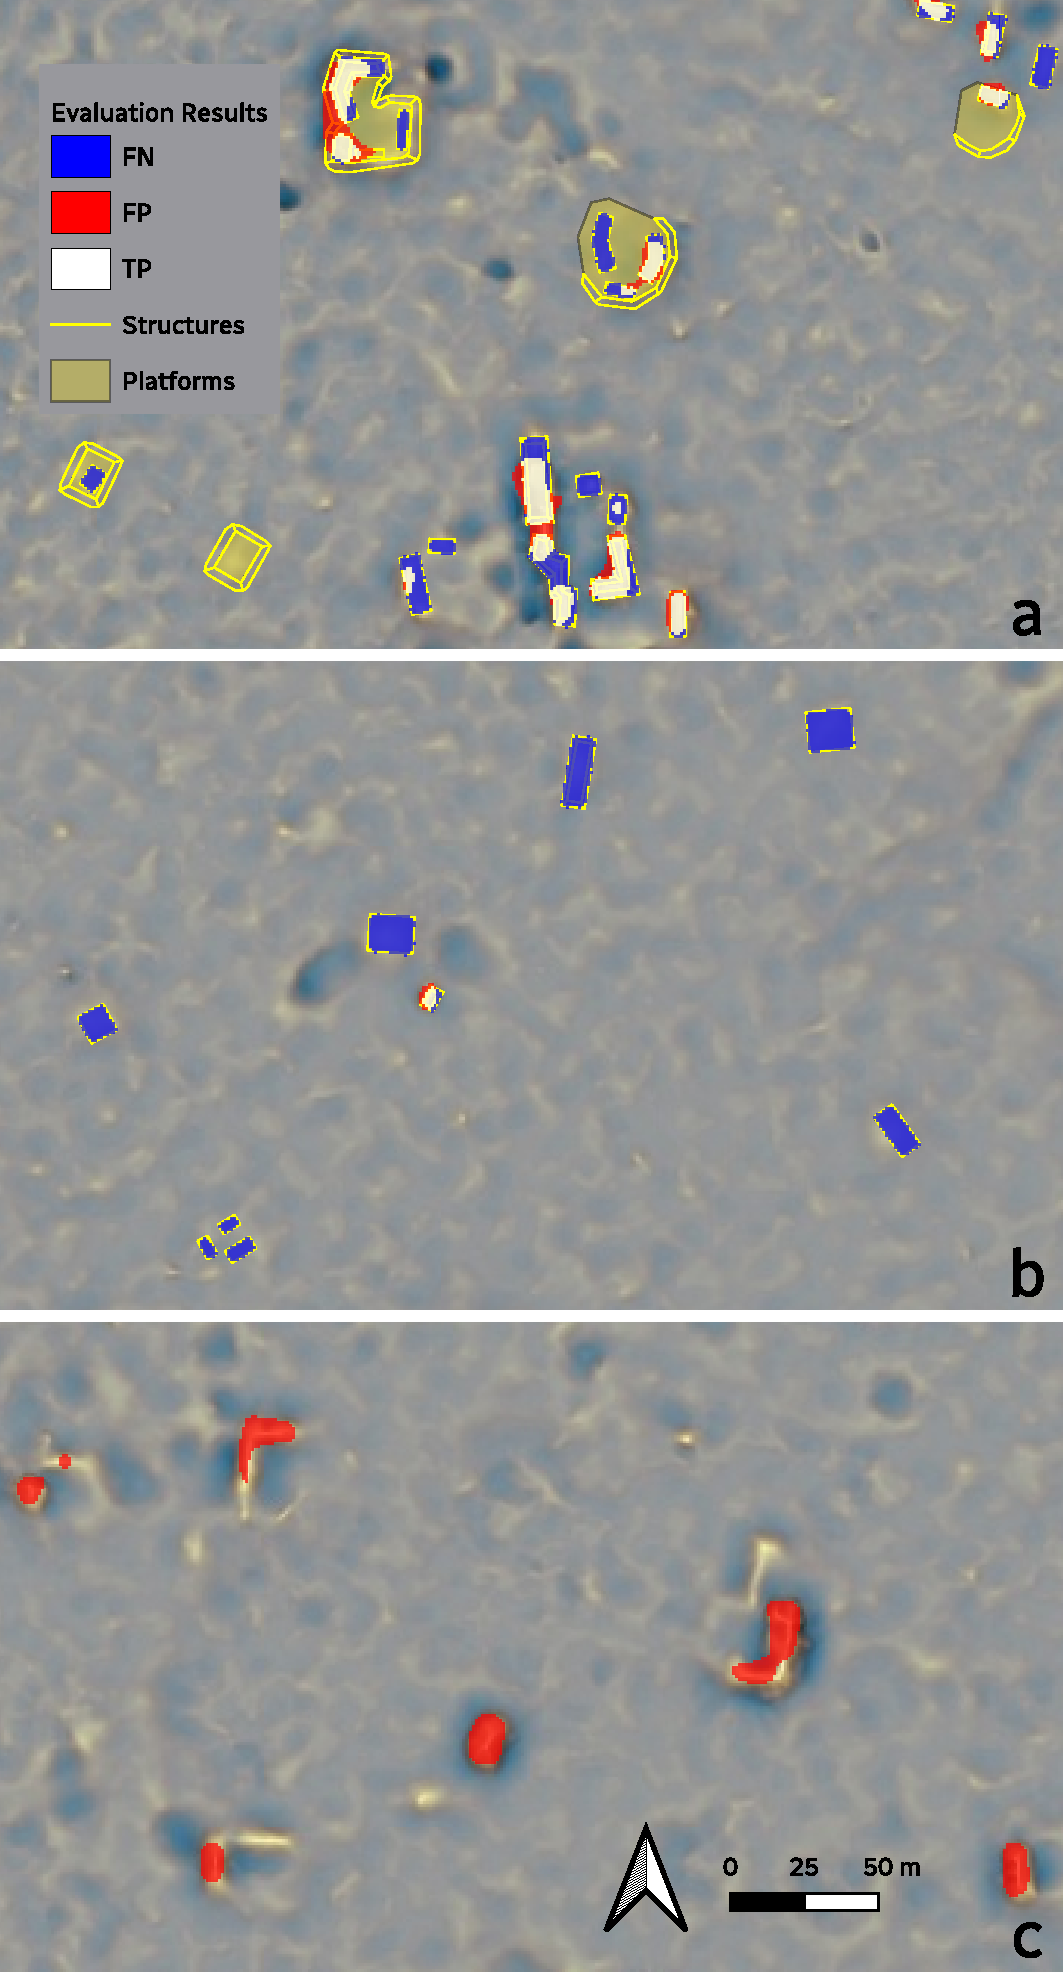
\includegraphics[width=\textwidth]{figures/maya_tp_fp_fn_sps_v3.pdf}
        \caption{DeepLab V3}
        \label{fig:maya_v3}
    \end{subfigure}
    \hfill
    \begin{subfigure}{0.49\textwidth}
        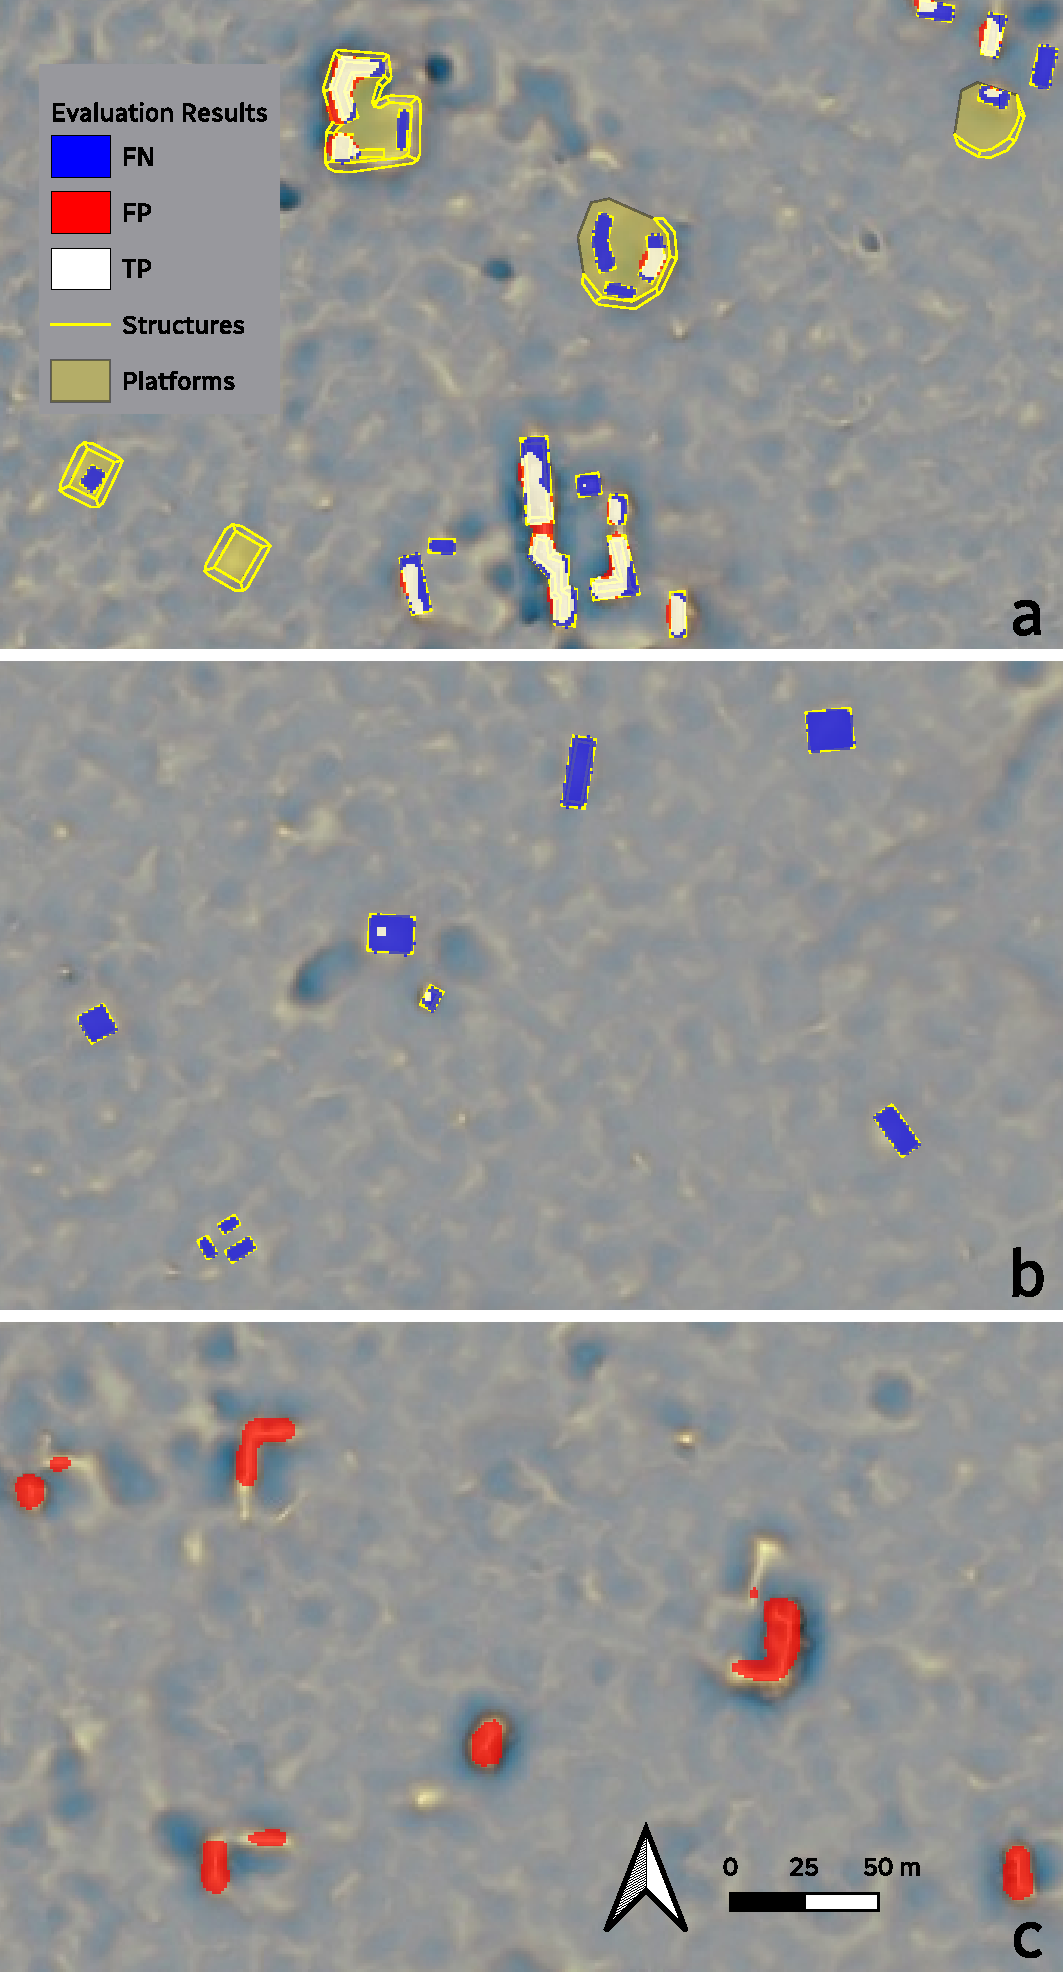
\includegraphics[width=\textwidth]{figures/maya_tp_fp_fn_sps_v3+.pdf}
        \caption{DeepLab V3+}
        \label{fig:maya_v3_plus}
    \end{subfigure}
    \caption{Comparison of the number of true positives, false positives, and false negatives for DeepLab V3 and DeepLab V3+ models on the Maya dataset.}
    \label{fig:maya_tp_fp_fn_comparison}
\end{figure}

\subsection{Best-Performing Configuration for Slovak Terraces}
\section{Ablation Study}
\subsection{Effect of Input Representation}
\subsection{Effect of Label Representation}
\subsection{Effect of Sampling Strategy}
\subsection{Effect of Loss Function}
\subsection{Effect of Tile Size of Inference Strategy}
\section{Error Analysis}
\section{Archaeological Usefulness of the Results}
\section{Limitations}

% !TEX root = ../thesis.tex

\chapter{Conclusion}\label{ch:conclusion}

\section{Summary of the Work}

This bachelor thesis addressed the problem of binary semantic segmentation of archaeological features in airborne LiDAR-derived raster data. The work was motivated by the fact that LiDAR data provide detailed information about terrain morphology, but their interpretation in archaeology still depends strongly on expert visual inspection. Since large LiDAR datasets are time-consuming to inspect manually, the thesis investigated whether deep learning can support archaeological interpretation by producing reproducible candidate maps of potential archaeological features.

The main objective was not only to train a segmentation model, but to design, implement, and experimentally evaluate a reproducible workflow for semantic segmentation in two different archaeological and geographical domains. The first domain consisted of compact Maya archaeological structures in Guatemala. The second domain consisted of terrace-like archaeological features in Slovakia. These two domains differ in object morphology, spatial resolution, annotation type, and terrain context. Their joint use therefore made it possible to evaluate not only the performance of the selected models, but also the sensitivity of the whole workflow to changes in data domain.

The thesis first analysed traditional and semi-automatic methods used in archaeological LiDAR interpretation and then reviewed the role of deep learning in remote sensing and archaeology. The analysis showed that deep learning methods are promising for archaeological prospection, but their practical usefulness depends on many methodological decisions. These include the choice of input representation, the conversion of expert annotations into training masks, the sampling strategy, the loss function, the model architecture, threshold optimization, post-processing, and the way in which the resulting maps are evaluated. For this reason, the work focused on building a controlled experimental framework rather than on presenting a single isolated model result.

A complete processing workflow was created. It included preparation of LiDAR-derived input representations, conversion of reference annotations into hard and soft masks, construction of tiled datasets, definition of train-validation strategies, model training, threshold-based inference, quantitative evaluation, and qualitative GIS-based inspection. The implemented workflow made it possible to compare several controlled variables under consistent conditions. In the Maya domain, the compared input representations included DEM, RGB-like visualization, RGDEM, and SPS. In the Slovak domain, DEM, ISO, and ANISO representations were evaluated. The work also compared hard and soft label variants, different tile sizes, selected loss functions, and DeepLab-based segmentation architectures.

The best-performing configuration for the Maya dataset was based on DeepLab~V3+ with an ImageNet-pretrained ResNet-101 backbone, SPS input representation, soft labels with a radius of 2~m, Tanimoto with complement loss, and $128 \times 128$ pixel tiles with a stride of 32 pixels. This configuration achieved stronger results than the earlier DeepLab~V3 baseline across the retained pixel-wise metrics. In particular, the foreground IoU increased from 0.24690 to 0.37924, the F1 score from 0.39602 to 0.54992, and the Matthews correlation coefficient from 0.39634 to 0.56307. From the object-level perspective, the selected DeepLab~V3+ configuration detected 2253 out of 4084 reference objects, while the compared DeepLab~V3 baseline detected 1746 objects. The improvement should therefore be interpreted primarily as an increase in detection completeness.

The best-performing configuration for the Slovak terrace dataset was based on DeepLab~V3+ with a ResNet-101 backbone, ANISO input representation, soft labels with a radius of 2~m, BCE+Dice loss, and $512 \times 512$ pixel tiles with a stride of 128 pixels. This configuration achieved the strongest overall performance among the evaluated Slovak variants. However, the Slovak results were substantially more difficult to interpret than the Maya results. The terrace features are narrow, elongated, partially discontinuous, and represented by buffered polylines rather than precise polygonal outlines. As a result, the model often detected broader terrace-like zones rather than individual terrace lines. The obtained foreground IoU of 0.06560 and F1 score of 0.12313 show that the output is not suitable as a final segmentation map. Nevertheless, the object-level hit rate of 16 detected objects out of 24 indicates that the model can still be useful as a candidate localization layer.

The ablation study showed that LiDAR-derived input representation has a clear influence on segmentation quality. On the Maya dataset, SPS achieved the strongest results among the compared representations, while DEM produced the weakest result. This confirms that direct elevation values alone are less informative for this task than representations that emphasize local terrain morphology. The comparison of hard and soft labels showed a more nuanced result. Soft masks did not improve all configurations uniformly, but they often increased recall and reduced precision. This behaviour is useful when the main goal is to avoid missing potential archaeological candidates, but it also increases the risk of false-positive predictions. The tile-size experiments showed that smaller tiles were more suitable for compact Maya structures, while a larger tile size was more appropriate for Slovak terraces, where broader terrain context is needed. The loss-function comparison showed that BCE+Dice produced the strongest metric-oriented result in one comparison group, while Tanimoto with complement provided more stable training behaviour and was used in the strongest Maya configuration. The architecture comparison showed that DeepLab~V3+ was preferable to DeepLab~V3 because it provided a slightly better precision-recall balance and more stable behaviour.

The qualitative error analysis showed that the trained models do not fail randomly. False-positive predictions usually occurred on natural or disturbed terrain forms that visually resembled archaeological structures. False-negative predictions were especially common for small, isolated, weakly preserved, or low-contrast objects. Boundary errors appeared when the model localized a relevant structure but did not reproduce the full reference outline. This behaviour reflects an important property of archaeological LiDAR segmentation: expert annotations do not always correspond exactly to the currently visible terrain expression. The model tends to follow the raster-visible relief signal, while the annotation may represent an interpreted archaeological object. Therefore, some metric penalties reflect not only model error, but also uncertainty in the relation between the terrain representation and the reference geometry.

The archaeological usefulness of the results depends on the intended use case. For the Maya dataset, the model is useful mainly as a candidate detector, especially for medium and large structures. Large structures were detected most reliably, with 400 detected objects out of 472 and a hit rate of 0.8475. Medium-sized structures were detected with a hit rate of 0.6338, while small structures reached only 0.3287. This confirms that object size and terrain expression strongly influence detectability. For the Slovak terrace dataset, the model is not suitable for automatic extraction of precise terrace geometries, but it can highlight probable terrace zones. In both cases, the output should be interpreted as a decision-support layer for expert-guided inspection rather than as an automatic archaeological inventory.

\section{Fulfilment of Objectives}

The main objective of the thesis was fulfilled. A reproducible deep learning workflow for binary semantic segmentation of archaeological features in airborne LiDAR-derived raster data was designed, implemented, and experimentally evaluated. The workflow was applied to two different domains: Maya archaeological structures in Guatemala and terrace-like archaeological features in Slovakia. The experiments demonstrated that the same general workflow can be used in both domains, but also showed that domain-specific adjustment is necessary.

The first partial objective was to analyse the current state of remote sensing, LiDAR-based archaeological prospection, and deep learning methods used for archaeological object detection and semantic segmentation. This objective was fulfilled in the analytical part of the thesis. The work described the transition from traditional remote sensing and manual LiDAR interpretation toward semi-automatic and deep learning-based methods. It also identified the main methodological problems relevant to this thesis: input representation, label uncertainty, class imbalance, and the difference between numerical segmentation quality and archaeological usefulness.

The second partial objective was to prepare LiDAR-derived input representations suitable for CNN-based semantic segmentation. This objective was fulfilled by preparing and evaluating several raster representations derived from the available terrain data. For the Maya dataset, DEM, RGB-like visualization, RGDEM, and SPS were compared. For the Slovak dataset, DEM, ISO, and ANISO representations were used. The results showed that input representation is one of the most important components of the workflow. In the Maya experiments, SPS provided the strongest performance, while DEM was the weakest representation. This confirms that derived terrain visualizations can provide more useful information for segmentation than direct elevation values alone.

The third partial objective was to prepare reference masks for both study domains and to compare hard binary labels with soft label variants. This objective was fulfilled by converting the available expert annotations into raster masks and by constructing both hard and soft label representations. The experiments showed that soft masks are not universally better than hard masks. Their most visible effect was a shift in the precision-recall balance: they often increased recall while reducing precision. This means that soft labels can be useful when the priority is to increase candidate coverage, but they must be used carefully because broader predictions may also increase false positives.

The fourth partial objective was to construct a reproducible tiled dataset pipeline based on manifests, valid-pixel masks, controlled spatial splits, and consistent train-validation strategies. This objective was fulfilled through the dataset construction workflow. Raster data and masks were divided into tiles and organized into controlled experimental subsets. This made it possible to compare model configurations systematically and to reduce the risk that differences in results were caused by changes in data preparation rather than by the tested methodological component.

The fifth partial objective was to train and compare selected semantic segmentation models on the Maya and Slovak datasets under controlled experimental settings. This objective was fulfilled by training DeepLab-based models on both study domains and comparing their performance using consistent metrics. The work compared DeepLab~V3 and DeepLab~V3+ variants, including pretrained and non-pretrained configurations. The strongest Maya configuration used DeepLab~V3+ with an ImageNet-pretrained ResNet-101 backbone, while the strongest Slovak configuration used DeepLab~V3+ with a ResNet-101 backbone trained from scratch. These results show that the most appropriate model setup depends on the domain and the morphology of the target objects.

The sixth partial objective was to evaluate the influence of input representation, label type, sampling strategy, loss function, model architecture, and post-processing on segmentation performance. This objective was fulfilled through the ablation study and the comparison of representative configurations. The experiments showed that SPS was the strongest Maya input representation, that soft labels mainly affected the recall-precision balance, that tile size must be selected according to object morphology and raster resolution, that loss functions differ not only in final metrics but also in training stability, and that DeepLab~V3+ is preferable to DeepLab~V3 in the evaluated setup. The results therefore identify which workflow components had a clear impact and which effects were more limited or domain-dependent.

The seventh partial objective was to assess the obtained results using both quantitative pixel-wise metrics and qualitative inspection in a GIS environment. This objective was fulfilled. Pixel-wise metrics such as foreground IoU, F1 score, precision, recall, balanced accuracy, and Matthews correlation coefficient were used for controlled comparison. At the same time, qualitative GIS-based inspection was used to interpret false positives, false negatives, boundary errors, and successful predictions. This combined evaluation was necessary because pixel-level metrics alone do not fully describe whether a prediction is archaeologically useful.

The eighth partial objective was to identify representative configurations that either improve segmentation quality or clearly demonstrate limitations of the proposed workflow. This objective was fulfilled in the results and discussion. The best-performing Maya and Slovak configurations were identified, and weaker or more ambiguous configurations were discussed through the ablation study. The analysis also identified the main limitations of the workflow, including reference-data uncertainty, extreme class imbalance, limited cross-domain generalization, differences in object morphology, and the need for expert interpretation of full-area inference results.

The research questions defined in the thesis were also addressed. The experiments showed that LiDAR-derived input representation has a substantial effect on segmentation quality, that visually enhanced raster representations can outperform direct DEM input, and that combining or deriving terrain features can improve model performance when the representation emphasizes relevant micro-relief. The comparison of hard and soft labels showed that label representation influences training behaviour and prediction selectivity. The loss-function experiments showed that different objectives lead to different precision-recall behaviour and training stability. The model comparison showed that DeepLab~V3+ is generally preferable in the tested setting, but that architecture alone is not the only determining factor. Finally, the GIS-based analysis confirmed that the best pixel-wise results do not automatically equal a final archaeological interpretation. The most useful outputs are those that can support expert inspection by highlighting candidate areas.

\section{Main Contributions}

The first contribution of this thesis is the design and implementation of a reproducible workflow for semantic segmentation of archaeological features in LiDAR-derived raster data. The workflow connects geospatial data preparation, reference mask generation, tiled dataset construction, model training, threshold-based inference, metric evaluation, and GIS-based interpretation. This is important because the quality of deep learning results in archaeological LiDAR analysis depends not only on the model architecture, but also on many preceding and following methodological steps.

The second contribution is the controlled comparison of several methodological components under a consistent experimental framework. The thesis did not treat the trained model as a black-box result. Instead, it evaluated the influence of input representation, label representation, tile size, loss function, and model architecture. This makes the results more informative than a single final score, because it shows which parts of the workflow influenced the final output and how these effects differed between the Maya and Slovak domains.

The third contribution is the experimental evaluation of different LiDAR-derived input representations. The results demonstrated that SPS was the most effective representation for Maya structures among the tested variants, while DEM was the weakest. This confirms that representations emphasizing local terrain morphology are more useful for this segmentation task than direct elevation values alone. For the Slovak dataset, the best-performing configuration used ANISO, which indicates that the optimal representation depends on the morphology of the target objects and the landscape context.

The fourth contribution is the evaluation of hard and soft label representations for archaeological segmentation. The thesis showed that soft labels can be useful, but their effect is not uniformly positive. They can increase recall and make the model more inclusive, but this may reduce precision and increase false positives. This result is important because archaeological annotations are often uncertain, schematic, or spatially imprecise. Soft labels can partly address this problem, but they do not remove the need for careful interpretation of prediction boundaries.

The fifth contribution is the evaluation of the practical archaeological usefulness of the predictions, not only their pixel-wise quality. For the Maya dataset, the best model detected 2253 out of 4084 reference objects. The size-based analysis showed that the model was much more reliable for large and medium-sized structures than for small structures. This result provides a more archaeologically meaningful interpretation than pixel-level metrics alone. For the Slovak terrace dataset, the model detected 16 out of 24 terrace objects, but the qualitative analysis showed that the output should be interpreted as candidate localization rather than precise delineation.

The sixth contribution is the identification of the main error types in archaeological LiDAR segmentation. The thesis distinguished false positives, false negatives, and boundary errors and related them to terrain morphology, label uncertainty, object size, and visualization effects. This analysis showed that many false positives appear in areas that are visually similar to archaeological structures, while false negatives are common for small or weakly expressed objects. Boundary errors often reflect the mismatch between expert-interpreted object outlines and the visible terrain signal. These observations are important for understanding how model outputs should be used in practice.

The seventh contribution is the comparison of two different archaeological domains within the same methodological framework. The Maya and Slovak datasets differ substantially in morphology and annotation type. The Maya dataset contains compact archaeological structures, while the Slovak dataset contains narrow and elongated terrace-like features. The results showed that a workflow suitable for one domain cannot be transferred directly to another without adjustment. This supports the conclusion that archaeological deep learning workflows require domain-specific validation.

The final contribution is the formulation of a realistic interpretation of the role of deep learning in archaeological LiDAR prospection. The thesis does not claim that the developed models replace expert interpretation. Instead, it shows that semantic segmentation can be useful as a decision-support tool. The strongest results are suitable for highlighting candidate locations and reducing the amount of terrain that must be inspected manually, especially in the case of medium and large Maya structures and broader Slovak terrace zones. The final archaeological interpretation, however, remains dependent on expert review.

\section{Future Work}

Several directions for future work follow directly from the limitations and results of this thesis.

The first direction is the improvement of reference data. The experiments showed that reference annotations strongly influence both model training and evaluation. Future work should therefore focus on producing more consistent expert annotations, documenting uncertainty in the labels, and distinguishing between visible terrain expression and interpreted archaeological extent. For the Slovak terrace dataset, more precise polygonal annotations or several alternative label representations could help clarify whether the model fails because of weak terrain signal, unsuitable architecture, or mismatch between buffered polylines and actual relief morphology.

The second direction is the extension of the evaluation protocol. Pixel-wise metrics are necessary, but they are not sufficient for archaeological interpretation. Future work should further develop object-level and GIS-based evaluation methods that better reflect archaeological usefulness. In particular, candidate localization, distance from reference features, object size, connected components, and expert review categories may provide more informative assessment than foreground IoU alone. Such evaluation would be especially useful for terrace systems, where a prediction can indicate the correct area even if it does not overlap precisely with the reference line.

The third direction is the development of more domain-specific architectures and training strategies. This thesis evaluated selected DeepLab-based models, but the results suggest that archaeological LiDAR segmentation may benefit from architectural adjustments. For compact Maya structures, models that preserve local boundary detail may improve delineation. For Slovak terraces, models better adapted to narrow, elongated, and discontinuous features may be necessary. Future experiments may therefore investigate architectures with stronger multiscale feature fusion, attention mechanisms, higher-resolution decoders, or methods designed specifically for thin linear objects.

The fourth direction is the comparison of semantic segmentation with object detection and instance segmentation approaches. This thesis was limited to binary semantic segmentation. However, the results show that object-level usefulness is sometimes more important than exact pixel-wise overlap. For Maya structures, instance-level methods could help separate individual structures. For Slovak terraces, object detection or line-aware methods could be more appropriate than dense binary segmentation if the goal is candidate localization rather than exact mask extraction.

The fifth direction is improved handling of class imbalance and false positives. Archaeological features occupy only a small fraction of the raster area, and this creates a strong foreground-background imbalance. Future work should further investigate sampling strategies, loss functions, and post-processing methods that improve recall without producing excessive false positives. This is especially important for full-area inference, where a large number of false-positive candidates can reduce the practical usefulness of the model.

The sixth direction is broader cross-domain validation. The two datasets used in this thesis already demonstrated that results depend strongly on data domain. Future work should therefore test the workflow on additional archaeological contexts, additional terrain types, and additional annotation styles. Such validation would help determine which conclusions are specific to the Maya and Slovak datasets and which methodological findings can be generalized to other LiDAR-based archaeological prospection tasks.

The seventh direction is the integration of the model outputs into a human-in-the-loop archaeological workflow. Since the model outputs are most useful as candidate layers, future work should focus on how predictions can be reviewed, corrected, and reused by experts. A practical workflow could combine probability maps, binary masks, object candidates, uncertainty indicators, and GIS-based editing. Expert corrections could then be incorporated into later training iterations, gradually improving the dataset and the model.

The final direction is the possible extension beyond raster-derived products. This thesis worked only with LiDAR-derived raster representations and did not process the original point clouds directly. Future research may compare raster-based segmentation with methods that use point-cloud information or additional terrain derivatives. Such work would be beyond the scope of the present thesis, but it may help determine whether some weakly expressed archaeological features are better represented before rasterization or through alternative terrain models.

In conclusion, the thesis demonstrated that deep learning can support archaeological LiDAR interpretation, but only within a carefully controlled and expert-guided workflow. The obtained results are not sufficient for fully automatic archaeological mapping. They are, however, useful for candidate detection and prioritization, especially when the target structures have clear terrain expression. The main value of the work lies in showing how methodological decisions influence the final segmentation output and in defining the conditions under which model predictions can be meaningfully used in archaeological prospection.


%% Bibliography, glossary, acronyms
\backmatter{}


%% -----------------------------------------------------------------
%%                                       _ _
%%       __ _ _ __  _ __   ___ _ __   __| (_) ___ ___  ___
%%      / _` | '_ \| '_ \ / _ \ '_ \ / _` | |/ __/ _ \/ __|
%%     | (_| | |_) | |_) |  __/ | | | (_| | | (_|  __/\__ \
%%      \__,_| .__/| .__/ \___|_| |_|\__,_|_|\___\___||___/
%%           |_|   |_|
%% -----------------------------------------------------------------

% !TEX root = ../thesis.tex

\chapter*{\appendixlistname}
\addcontentsline{toc}{chapter}{\appendixlistname}

\begin{description}

   \item[\autoref{app:user.manual}] \nameref{app:user.manual}
   \item[\autoref{app:system.manual}] \nameref{app:system.manual}
   \item[\autoref{app:suplementary.material}] \nameref{app:suplementary.material}
   \item[\autoref{app:ai_tools}] \nameref{app:ai_tools}
   \item[\appendixname{} E] CD drive -- Electronic version of the thesis:
   \begin{itemize}
    \item \texttt{doc} -- the thesis, appendices and latex sources
    \item \texttt{src} -- source codes of the developed solution
   \end{itemize}


\end{description}


\appendix
\setappendixstyle


% !TEX root = ../thesis.tex

\chapter{User Manual}\label{app:user.manual}

\begin{sloppypar}

This user manual describes how to use the implemented information output of the thesis: a reproducible Python pipeline for binary semantic segmentation of archaeological features in LiDAR-derived raster data.

The pipeline is intended for experiments with prepared raster datasets, training segmentation models, evaluating trained checkpoints, and generating full-area \gls{probabilitymap}. It is not an interactive desktop application. The expected user is therefore a researcher or student who can run Python scripts from a command line and who has access to the prepared data files.

\section{Repository and Directory Structure}

The source repository is available as:

\begin{verbatim}
https://github.com/kitnew/lidar-archaeology-segmentation.git
\end{verbatim}

The most important directories are:

\begin{description}
    \item[\texttt{thesis/src/}] Python source code for datasets, models, training, evaluation, inference, losses, and metrics.
    \item[\texttt{thesis/configs/}] Hydra configuration files defining datasets, models, losses, paths, and experiment parameters.
    \item[\texttt{thesis/data/processed/}] Expected location of prepared \texttt{.npz} raster datasets and tile \gls{datasetmanifest}. The data files are not distributed through Git because of size and privacy constraints.
    \item[\texttt{thesis/outputs/}] Default location for trained checkpoints, Hydra logs, and generated prediction files.
    \item[\texttt{thesis/notebooks/} and \texttt{thesis/notebooks/scripts/}] Helper notebooks and scripts used during data preparation and visualization.
\end{description}

\section{System Requirements}

The pipeline was developed for Linux and Python. GPU execution with CUDA is expected for training and evaluation. The training script explicitly selects \texttt{cuda}, therefore a CUDA-capable environment is required for normal training runs.

The main software requirements are Python 3.8 or newer, PyTorch, Torchvision, Hydra, OmegaConf, NumPy, Pandas, Pillow, Matplotlib, \gls{gdal}, tqdm, and segmentation-models-pytorch for DeepLabV3+ experiments. The repository contains \texttt{requirements.txt} and \texttt{pyproject.toml}; however, the exact PyTorch and CUDA builds should be installed according to the target machine.

\section{Installation}

After cloning the repository, create and activate a virtual environment:

\begin{verbatim}
python -m venv .venv
source .venv/bin/activate
pip install -r requirements.txt
\end{verbatim}

If DeepLabV3+ configurations are used, install \texttt{segmentation-models-pytorch}. If the local \texttt{requirements.txt} does not include PyTorch, install the correct PyTorch, Torchvision, and CUDA build for the machine before running the pipeline.

\section{Input Data}

The training and inference scripts expect prepared NumPy archives and tile \gls{datasetmanifest}. A prepared dataset archive normally contains:

\begin{itemize}
    \item \texttt{data}: raster input tensor with shape \texttt{(C, H, W)};
    \item \texttt{valid}: valid-data mask with shape \texttt{(H, W)};
    \item \texttt{mask}: binary reference mask with shape \texttt{(H, W)};
    \item \texttt{soft\_mask}: optional soft reference mask used for training when enabled;
    \item \texttt{meta}: optional geospatial metadata.
\end{itemize}

The \gls{datasetmanifest} file, usually \texttt{.parquet}, contains the tile coordinates, tile size, subset assignment, validity fraction, and whether the tile contains positive pixels. Dataset variants are selected through files in \texttt{configs/dataset/}.

Before running experiments, set the data root so Hydra resolves paths correctly:

\begin{verbatim}
export DATA_ROOT=/path/to/project/data/processed
export OUTPUT_DIR=./outputs
export LOG_DIR=./logs
\end{verbatim}

\section{Training a Model}

Training is started from the repository root:

\begin{verbatim}
python -u src/train.py
\end{verbatim}

The default configuration is read from \texttt{configs/train.yaml}. It can be overridden from the command line. For example, to train a DeepLabV3+ model with a specific dataset and loss:

\begin{verbatim}
python -u src/train.py \
  dataset=sps_10_shadowed_2 \
  model=deeplabv3plus/resnet101_pretrained \
  loss=binarytanimoto \
  batch_size=16 \
  epochs=100
\end{verbatim}

Hydra creates a separate output directory for each run. The best checkpoint is saved as \texttt{best\_model.pth}. By default, the checkpoint is selected by positive-class \gls{iou}, but the configuration can use \gls{f1} instead through \texttt{checkpoint\_metric}.

\section{Evaluation}

Evaluation reconstructs a validation \gls{probabilitymap} from overlapping tiles, searches for an optimal threshold, and prints segmentation metrics. Run:

\begin{verbatim}
python -u src/evaluation.py \
  checkpoint_path=/path/to/best_model.pth \
  dataset=terraces_aniso_ladzany_128_32
\end{verbatim}

The evaluation output includes the optimal threshold and metrics such as positive \gls{iou}, mean \gls{iou}, Precision, Recall, \gls{f1}, specificity, accuracy, and \texttt{MOR10R}. The metrics are computed only over valid pixels and over regions actually covered by validation tiles.

\section{Full-Area Inference}

Inference generates a full \gls{probabilitymap} without requiring ground-truth labels. Run:

\begin{verbatim}
python -u src/inference.py \
  checkpoint_path=/path/to/best_model.pth \
  dataset=terraces_aniso_ladzany_full \
  output_path=outputs/inference/ladzany_probability_map.npy
\end{verbatim}

The output is a single-channel \texttt{.npy} array with probabilities in the range from 0 to 1. A \gls{binaryprediction} can be obtained by thresholding this array. The threshold may be the default value from \texttt{configs/inference.yaml}, a threshold found during evaluation, or a task-specific value chosen for visual \gls{gis} inspection.

\section{Running on a SLURM Cluster}

The repository contains \texttt{run\_slurm.slurm}, which demonstrates a cluster run. Before submitting it, update paths to the virtual environment and data directory. A typical submission is:

\begin{verbatim}
sbatch run_slurm.slurm
\end{verbatim}

The script exports \texttt{DATA\_ROOT}, \texttt{OUTPUT\_DIR}, and \texttt{LOG\_DIR}, activates the virtual environment, and starts \texttt{src/train.py} through \texttt{srun}.

\section{Correct Use and Limitations}

The pipeline assumes that all rasters, masks, and \gls{datasetmanifest} are spatially aligned. Incorrect alignment between the input raster and mask will produce invalid training data even if the scripts run without errors. For Slovak terraces experiments, the selected held-out location in the dataset configuration must match the intended leave-one-location-out fold.

The generated \gls{probabilitymap} should be interpreted as model outputs, not as verified archaeological discoveries. They should be checked against the original LiDAR-derived visualizations and, where possible, reviewed by a domain expert in a \gls{gis} environment.

\end{sloppypar}

% !TEX root = ../thesis.tex

\chapter{System Manual}\label{app:system.manual}

\begin{sloppypar}

This system manual describes the internal structure of the implemented information output. It follows the KKUI thesis documentation requirement that the system documentation should contain generated and commented source code or, at minimum, a commented and explained description of the principal methods and functions of the result. Because the complete source code is available in the repository, this appendix focuses on the main modules, their responsibilities, and the behaviour of the essential classes and functions.

\section{Overall Architecture}

The implementation is organized as a Hydra-configurable Python pipeline. Configuration files define which dataset, model, \gls{lossfunction}, and runtime paths are used. The executable scripts in \texttt{src/} instantiate these components and perform training, validation, evaluation, or inference.

\begin{description}
    \item[\texttt{src/train.py}] Main training entry point.
    \item[\texttt{src/evaluation.py}] Validation-map reconstruction and \gls{thresholdbasedinference} evaluation.
    \item[\texttt{src/inference.py}] Full-area \gls{tile} inference and probability-map export.
    \item[\texttt{src/datasets/}] Dataset classes for loading prepared raster archives and extracting \gls{tile}.
    \item[\texttt{src/models/}] Model factories for DeepLabV3 and DeepLabV3+.
    \item[\texttt{src/engine/}] Training loop, losses, and metric aggregation.
    \item[\texttt{src/utils/}] Helper functions for channel statistics and segmentation metrics.
\end{description}

\section{Configuration Layer}

Hydra is used to keep experiment definitions outside the source code. The top-level files \texttt{configs/train.yaml}, \texttt{configs/evaluate.yaml}, and \texttt{configs/inference.yaml} define defaults and runtime parameters. Dataset definitions are stored in \texttt{configs/dataset/}; they specify the dataset class, input \texttt{.npz} files, \gls{datasetmanifest} file, subset, \gls{tile} filtering, and cross-validation location.

The path configuration is stored in \texttt{configs/paths/default.yaml}. It resolves:

\begin{itemize}
    \item \texttt{DATA\_ROOT} to the processed data directory;
    \item \texttt{OUTPUT\_DIR} to experiment outputs;
    \item \texttt{LOG\_DIR} to logs.
\end{itemize}

This separation makes the same source code usable on a local workstation and on a cluster by changing environment variables or Hydra command-line overrides.

\section{Training Entry Point}

The function \texttt{main} in \texttt{src/train.py} is decorated with:

\begin{verbatim}
@hydra.main(
    version_base=None,
    config_path="../configs",
    config_name="train"
)
\end{verbatim}

Its main responsibilities are:

\begin{enumerate}
    \item load and print the resolved Hydra configuration;
    \item select the \gls{cuda} device;
    \item set random seeds for Python, NumPy, and PyTorch;
    \item optionally initialize Weights and Biases logging;
    \item instantiate the model, datasets, \gls{lossfunction}, optimizer, and trainer;
    \item run the training loop and save checkpoints to the Hydra output directory.
\end{enumerate}

The model and datasets are created through \texttt{hydra.utils.instantiate}, so the training script does not need hard-coded knowledge of a specific dataset variant or architecture.

\section{Dataset Classes}

\subsection{SegmentationDataset}

\texttt{SegmentationDataset} in \texttt{src/datasets/dataset.py} is the main dataset class for single-area segmentation experiments, especially the Maya dataset variants. It reads a \gls{datasetmanifest} file, filters it by subset, validity fraction, and positive-\gls{tile} selection, then loads a prepared \texttt{.npz} data archive.

The class expects raster input in \texttt{(C, H, W)} format. During \texttt{\_\_getitem\_\_}, it crops one \gls{tile} using the stored \texttt{y}, \texttt{x}, and \texttt{tile\_size} values from the \gls{datasetmanifest} and returns a dictionary:

\begin{verbatim}
{
    "data":  input tensor, shape (C, H, W),
    "mask":  reference mask, shape (1, H, W),
    "valid": valid-pixel mask, shape (1, H, W),
    "coords": tile origin [y, x]
}
\end{verbatim}

For the training subset, the class can use \texttt{soft\_mask} when it is present in the archive. Validation and full inference use binary masks or dummy zero masks, respectively.

\subsection{TerassesSegmentationDataset}

\texttt{TerassesSegmentationDataset} supports multi-location \gls{slovakterrace} experiments. It accepts either a single data path or a dictionary mapping location identifiers such as \texttt{ladzany}, \texttt{sasovske}, \texttt{sitno}, and \texttt{tribec} to prepared archives.

The class implements the leave-one-location-out logic used in the thesis:

\begin{itemize}
    \item \texttt{subset=train}: use annotated locations except \texttt{held\_out\_location};
    \item \texttt{subset=val}: use only \texttt{held\_out\_location};
    \item \texttt{subset=full}: use \texttt{full\_location} for full-area inference.
\end{itemize}

It also supports optional negative-\gls{tile} subsampling through \texttt{neg\_to\_pos\_ratio}, which is useful for highly imbalanced terrace masks.

\subsection{Augmentation}

Training augmentation is implemented as synchronized transformations over the input \gls{tile}, mask, and valid mask. The shared augmentation includes horizontal flips, vertical flips, and rotations by multiples of 90 degrees. Applying the same geometric transform to all three tensors preserves alignment between raster data and labels.

\section{Model Factories}

\texttt{src/models/deeplab\_v3.py} defines \texttt{create\_model} for Torchvision DeepLabV3. It supports \gls{resnet}-50 and \gls{resnet}-101 \gls{backbone} and can optionally initialize the \gls{backbone} with ImageNet weights. The output layer is configured for one class, which corresponds to one-logit binary segmentation.

\texttt{src/models/deeplab\_v3\_plus.py} defines the equivalent factory for DeepLabV3+ using \texttt{segmentation-models-pytorch}. It supports configurable encoder names, input channel count, output class count, and optional ImageNet encoder weights.

\section{Loss Functions}

Losses are implemented in \texttt{src/engine/losses.py}. All principal losses share the same interface:

\begin{verbatim}
forward(logits, targets, valid=None) -> scalar loss
\end{verbatim}

The helper \texttt{\_prepare\_binary\_tensors} validates tensor shapes and converts masks to the correct type. The helper \texttt{\_masked\_mean} computes a mean loss only over valid pixels when a valid mask is provided.

The implemented losses are:

\begin{description}
    \item[\texttt{BCEDiceLoss}] Combines binary cross-entropy with Dice loss. It is a stable general-purpose option for binary segmentation.
    \item[\texttt{BinaryTanimotoWithComplementLoss}] Computes Tanimoto similarity for foreground and background and minimizes one minus their average score.
    \item[\texttt{BinaryFocalLoss}] Down-weights easy pixels and focuses learning on harder examples.
    \item[\texttt{FocalDiceLoss}] Combines focal loss with Dice loss.
    \item[\texttt{BinaryDECBLoss}] Binary adaptation of a class-balance-inspired loss that changes class weights according to effective sample counts within a batch.
\end{description}

\section{Trainer}

\texttt{Trainer} in \texttt{src/engine/trainer.py} encapsulates the training and validation loop.

\texttt{train\_epoch} switches the model to training mode, iterates over batches, computes logits, evaluates the configured loss, performs backpropagation, and updates model parameters.

\texttt{validate} switches the model to evaluation mode, computes validation loss, thresholds sigmoid probabilities, and accumulates \glspl{truepositive}, \glspl{falsepositive}, \glspl{falsenegative}, and true negatives over valid pixels.

\texttt{fit} controls the epoch loop. It logs training and validation losses, calculates metrics, and saves \texttt{best\_model.pth} when the selected checkpoint metric improves. The checkpoint contains the epoch number, model weights, optimizer state, positive \gls{iou}, and \gls{fscore}.

\section{Evaluation and Inference}

\texttt{src/evaluation.py} reconstructs a full validation \gls{probabilitymap} from \gls{tile} predictions. Overlapping predictions are accumulated and then averaged by a per-pixel count map. The final map is compared against the \gls{referencemask} only where pixels are valid and covered by validation \gls{tile}. The script then searches for an optimal threshold and reports metrics.

\texttt{src/inference.py} uses the same reconstruction idea for prediction without ground-truth labels. The central function \texttt{run\_inference} creates two global tensors: one for the accumulated probabilities and one for the number of predictions per pixel. Each \gls{tile} prediction is inserted back into its original spatial position using the stored \gls{tile} coordinates. The final \gls{probabilitymap} is:

\begin{verbatim}
final_map = pred_map / clamp(map_count, min=1)
\end{verbatim}

The result is saved as a single-channel NumPy array. This output can be thresholded, converted to \gls{geotiff} by helper scripts, or inspected in \gls{gis} software together with the original \gls{lidarderiveddata} raster.

\section{Extension Points}

The pipeline can be extended without changing the main scripts. A new dataset variant can be added by creating another file under \texttt{configs/dataset/}. A new model can be added by implementing a factory function and registering it in \texttt{configs/model/}. A new \gls{lossfunction} must implement the same \texttt{forward(logits, targets, valid=None)} interface so that it can be used by \texttt{Trainer} without additional changes.

\end{sloppypar}

% !TEX root = ../thesis.tex

\chapter{Tables}\label{app:tables}

\begin{landscape}
\begin{table}[p]
\centering
\scriptsize
\setlength{\tabcolsep}{3pt}
\renewcommand{\arraystretch}{1.25}

\begin{tabularx}{\linewidth}{
@{}
p{0.9cm}
p{2.6cm}
p{3.0cm}
p{4.4cm}
p{1.5cm}
p{3.0cm}
Y
@{}
}
\toprule
&
\textbf{Experiment Group} &
\textbf{Controlled component} &
\textbf{Compared variants} &
\textbf{\makecell{Number of\\configurations}} &
\textbf{Best configuration} &
\textbf{Main observation} \\
\midrule

\multirow{5}{*}{\rotatebox{90}{Maya}}
& Input Data Representation
& LiDAR-derived input
& DEM (raw); RGB; RGDEM (raw); RGDEM (z-score); SPS (z-score)
& 10
& SPS (z-score)
& SPS provided a broader spatial context and highlighted local elevation changes, improving the distinction between man-made structures and natural terrain. \\

& Label Representation
& Target mask type
& Binary hard mask; soft mask with radius = \{2, 4, 6\}
& 38
& Hard mask / soft mask radius = 2
& Soft masks did not significantly improve the evaluation metric, with differences typically within $\pm$2\%. However, they produced lower precision and higher recall, while smoothing validation fluctuations. \\

& Loss function
& Optimization objective
& BCE + Dice; Tanimoto with complement; Focal; Focal + Dice; DECB
& 12
& BCE + Dice / Tanimoto
& The losses showed similar metric trends. Tanimoto produced smoother validation behaviour, higher precision, lower recall, and more stable convergence. \\

& Sampling Strategy
& Tile size selection
& 128 (32); 256 (64)
& 4
& 128 (32)
& The difference was minimal, but 128-sized tiles had a higher positive-to-negative pixel ratio. \\

& Model Architecture
& Segmentation network / initialization
& DeepLab V3; DeepLab V3+; DeepLab V3+ pretrained
& 6
& DeepLab V3+
& DeepLab V3+ achieved slightly better results than DeepLab V3, although the difference was only a few percentage points. \\

\midrule

\multirow{5}{*}{\rotatebox{90}{Slovakia}}
& Input Data Representation
& LiDAR-derived input
& DEM (z-score); DEM (min-max); ISO; ANISO
& 5
& ANISO
& ISO and ANISO performed similarly, but ANISO demonstrated more stable training. \\

& Label Representation
& Target mask type
& Binary hard mask; soft mask with radius = \{2, 4, 6\}
& 2
& Soft mask radius = 2
& The control metrics were higher and more stable, but the loss also increased due to more activations near the hard mask boundaries. \\

& Loss function
& Optimization objective
& BCE + Dice; Tanimoto with complement
& 4
& Tanimoto
& Tanimoto provided higher stability, smoother control metrics, and lower error. \\

& Sampling Strategy
& Tile size selection
& 128 (32); 256 (64); 512 (128); 1024 (256)
& 4
& 512 (128)
& This setting achieved the best benchmark results and the lowest error, balancing resolution and tile context. \\

& Model Architecture
& Segmentation network / initialization
& DeepLab V3; DeepLab V3+; DeepLab V3+ pretrained
& 5
& DeepLab V3+
& The models produced similar results, but DeepLab V3+ improved when additional preprocessing was applied. Pretrained weights worked best with an appropriate loss function. \\

\bottomrule
\end{tabularx}

\caption{Overview of conducted experiments on Maya structures and Slovak terraces with outcomes.}
\label{app:tab:experiments_summary}
\end{table}
\end{landscape}
% !TEX root = ../thesis.tex

\chapter{AI Tools}\label{app:ai_tools}

This appendix provides a transparent overview of the artificial intelligence and \gls{ai}-assisted tools that were used during the preparation of this thesis. The purpose of this appendix is not to present these tools as part of the proposed methodological contribution, but to clearly distinguish between the author's own work and external \gls{ai}-assisted support used during literature search, workflow design, implementation support, debugging, and text refinement.

The use of \gls{ai}-assisted tools was limited to supportive, consultative, and organizational tasks. These tools were not used as autonomous decision-making systems and did not replace the author's responsibility for the research design, implementation, experimental evaluation, interpretation of results, or final academic writing. All methodological choices, experimental decisions, code integration, result interpretation, and final text approval remained under the author's control.

\section{General Principles of Use}

\gls{ai}-assisted tools were used according to the following principles:

\begin{itemize}
    \item \gls{ai} tools were used as auxiliary instruments for literature discovery, note enrichment, workflow consultation, code assistance, debugging, and language refinement.
    \item The tools did not independently define the research problem, objectives, experimental protocol, or final conclusions of the thesis.
    \item Generated code snippets were reviewed, adapted, and integrated manually by the author before being used in the project.
    \item Interpretations of experimental results were treated as suggestions and were checked against the measured metrics, generated visualizations, and the broader methodological context of the thesis.
    \item \gls{ai}-assisted textual edits were used for improving clarity, grammar, structure, and consistency, while the final meaning, argumentation, and responsibility for the text remained with the author.
    \item The tools were not used to fabricate sources, results, measurements, tables, or figures.
\end{itemize}

\section{ResearchRabbit}

ResearchRabbit was used as a literature discovery tool. It supported the search for relevant scientific articles and made it possible to explore citation networks between already identified publications. This was useful for detecting closely related works, following citation paths, and identifying papers that were methodologically or conceptually connected to the thesis topic.

In addition, ResearchRabbit helped trace the origin and usage context of several domain-specific terms encountered during the literature review. However, the tool was not used to determine the final relevance of a publication automatically. The final selection of sources was performed manually by reading, screening, and comparing the articles in the context of the thesis topic.

\section{NotebookLM}

NotebookLM was used for the preliminary analysis of a collected cluster of scientific articles. Its use started only after manual screening had already been performed. The tool helped summarize and compare selected papers and supported the identification of articles that were likely to be relevant for the analytical part of the thesis.

NotebookLM was also used to supplement manually created notes for individual articles. This was done in order to reduce the risk of overlooking details that could be important in the context of \gls{semanticsegmentation}, \gls{lidarderiveddata} visualizations, archaeological object detection, label uncertainty, \gls{classimbalance}, or evaluation methodology.

The tool was additionally used when preparing indirect citations. In such cases, NotebookLM helped identify whether a statement, although not explicitly formulated in a given article, was indirectly supported by the article's results, methodology, or discussion. These suggestions were not accepted automatically. The author verified the context manually before using such material in the thesis.

\section{Anara}

Anara was used only for the initial analysis of the root article by Bundzel et al., which served as one of the main starting points for understanding the domain-specific background of \gls{lidar}-based archaeological segmentation. Its use was limited to early familiarization with the article and did not replace the author's own reading, interpretation, or subsequent analysis of the publication.

\section{ChatGPT 5.4 Thinking Extended}

ChatGPT 5.4 Thinking Extended was used mainly as a consultative tool during the design of a reproducible research workflow. It supported the planning of a project structure that separated source code, data, configurations, experiment outputs, evaluation results, and thesis-related artifacts. This helped reduce the amount of time spent on organizational and implementation-related decisions and allowed greater focus on experimental design and result interpretation.

The tool was also useful during the initial analysis of experimental results. It helped formulate possible interpretations of measured metrics, compare experiment groups, and identify relationships between model architecture, \gls{inputrepresentation}, label representation, sampling strategy, \gls{lossfunction}, and observed performance.

In addition, ChatGPT 5.4 Thinking Extended was used to generate small code snippets for specific functions, pandas data frames for comparative result tables, and helper scripts for processing intermediate experiment outputs. It was also used for targeted debugging of code. All generated code was reviewed, modified, and tested by the author before being included in the workflow.

\section{ChatGPT 5.5 Thinking Extended}

ChatGPT 5.5 Thinking Extended was used during the later stages of thesis preparation. It supported discussion of experimental results, checking consistency between different sections of the thesis, identifying possible grammar issues, and improving the formulation of selected paragraphs.

The tool was also used to assist with the presentation of results, including the formatting of tables, graphs, figures, and explanatory text. Its role was editorial and consultative. It did not replace the author's responsibility for the results, interpretation, structure, or final wording of the thesis.

\section{Boundaries of AI Assistance}

The use of \gls{ai}-assisted tools did not include the following:

\begin{itemize}
    \item autonomous formulation of the thesis objectives;
    \item autonomous selection of the final methodology;
    \item independent implementation of the complete experimental pipeline;
    \item automatic generation of experimental results;
    \item fabrication or invention of citations, metrics, tables, or figures;
    \item replacement of manual validation of code, results, and written claims;
    \item replacement of the author's interpretation of the archaeological and machine-learning relevance of the results.
\end{itemize}

The final thesis therefore remains the author's own academic work. \gls{ai}-assisted tools were used only as supporting instruments for literature exploration, workflow organization, implementation assistance, debugging, language refinement, and critical discussion of results.


% avoid empty lof, lot and lol
\setcounter{figure}{0}
\setcounter{table}{0}
\setcounter{lstlisting}{0}


%% -----------------------------------------------------------------
%%       ___ _   _ _ __ ___   _____   __
%%      / _ \ | | | '__/ _ \ / __\ \ / /
%%     |  __/ |_| | | | (_) | (__ \ V /
%%      \___|\__,_|_|  \___/ \___| \_/
%% -----------------------------------------------------------------

% Životopis autora
% \curriculumvitae\protect
% Táto časť je nepovinná. Autor tu môže uviesť svoje biografické
% údaje, údaje o~záujmoch, účasti na~projektoch, účasti na~súťažiach,
% získané ocenenia, zahraničné pobyty na~praxi, domácu prax, publikácie
% a~pod.

\end{document}
